%\documentclass[compress]{beamer}
\documentclass[8pt]{beamer}

%-----------------------------------------------------------
% PACKAGES

%\usepackage[latin1]{inputenc}
\mode<presentation>

%\usepackage[T1]{fontenc}  
\usetheme{Warsaw}
%\usetheme{Madrid}

\usepackage{graphicx}
%\usepackage[section]{placeins} % force � mettre l'image o� on veut
%\usepackage{float} %utiliser H pour forcer � mettre l'image o� on veut
%\usepackage{lscape} %utilisation du mode paysage
%\usepackage{pslatex}
\usepackage{url}
\usepackage{subfigure}
\usepackage{caption}
%\usepackage{subcaption}
%\usepackage[caption=false]{subfig}

\usepackage{graphicx}
\usepackage{tabls}
\usepackage{afterpage}

%\usepackage[]{media9}
%\usepackage{multimedia}

\usepackage{amsthm}
\usepackage{amssymb}
\usepackage{amsmath}
\usepackage{amsfonts}
\usepackage{amstext}
\usepackage{amsbsy}
\usepackage{mathbbol} 


\usepackage{epsfig}
%\usepackage{epsfig}
%\usepackage{cites}
\usepackage{epsf}
\usepackage{array}
\usepackage{color}

%-----------------------------------------------------------
% NEW  DEFINITIONS
%
%=================================================================================================
% new commands
% +++++++++++++++++++++++++++++++++++++++++++++++++++++++++++++++++++++++++++++++++++++++++++++++++
\newcommand{\nc}{\newcommand}

% operators
\renewcommand{\div}{\mbold{\nabla}\! \cdot \!}
\newcommand{\grad}{\mbold{\nabla}}
\newcommand{\divv}[1]{\boldsymbol{\nabla}^{#1}\! \cdot \!}
\newcommand{\gradd}[1]{\mbold{\nabla}^{#1}}
\newcommand{\mbold}[1]{\boldsymbol#1}
% latex shortcuts
\newcommand{\bea}{\begin{eqnarray}}
\newcommand{\eea}{\end{eqnarray}}
\newcommand{\be}{\begin{equation}}
\newcommand{\ee}{\end{equation}}
\newcommand{\bal}{\begin{align}}
\newcommand{\eali}{\end{align}}
\newcommand{\bi}{\begin{itemize}}
\newcommand{\ei}{\end{itemize}}
\newcommand{\ben}{\begin{enumerate}}
\newcommand{\een}{\end{enumerate}}
\usepackage{amsthm}
\newtheorem*{remark}{Remark}
% DGFEM commands
\newcommand{\jmp}[1]{[\![#1]\!]}                     % jump
\newcommand{\mvl}[1]{\{\!\!\{#1\}\!\!\}}             % mean value
\newcommand{\keff}{\ensuremath{k_{\textit{eff}}}\xspace}
% shortcut for domain notation
\newcommand{\D}{\mathcal{D}}
% vector shortcuts
\newcommand{\vo}{\mbold{\Omega}}
\newcommand{\vr}{\mbold{r}}
\newcommand{\vn}{\mbold{n}}
\newcommand{\vnk}{\mbold{\mathbf{n}}}
\newcommand{\vj}{\mbold{J}}
\newcommand{\eig}[1]{\| #1 \|_2}
%
\newcommand{\EI}{\mathcal{E}_h^i}
\newcommand{\ED}{\mathcal{E}_h^{\partial \D^d}}
\newcommand{\EN}{\mathcal{E}_h^{\partial \D^n}}
\newcommand{\ER}{\mathcal{E}_h^{\partial \D^r}}
\newcommand{\reg}{\textit{reg}}
%
\newcommand{\norm}{\textrm{norm}}
\renewcommand{\Re}{\textrm{Re}}
\newcommand{\Pe}{\textrm{P\'e}}
\renewcommand{\Pr}{\textrm{Pr}}
%
\newcommand{\resi}{R}
%\newcommand{\resinew}{\tilde{D}_e}
\newcommand{\resinew}{\widetilde{\resi}}
\newcommand{\resisource}{\widetilde{\resi}^{source}}
\newcommand{\matder}[1]{\frac{\textrm{D} #1}{\textrm{D} t}}
%
% extra space
\newcommand{\qq}{\quad\quad}
% common reference commands
\newcommand{\eqt}[1]{Eq.~(\ref{#1})}                     % equation
\newcommand{\fig}[1]{Fig.~\ref{#1}}                      % figure
\newcommand{\tbl}[1]{Table~\ref{#1}}                     % table
\newcommand{\sct}[1]{Section~\ref{#1}}                   % section
\newcommand{\app}[1]{Appendix~\ref{#1}}                   % appendix
%
\newcommand{\ie}{i.e.,\@\xspace}
\newcommand{\eg}{e.g.,\@\xspace}
\newcommand{\psc}[1]{{\sc {#1}}}
\newcommand{\rs}{\psc{R7}\xspace}
%
\newcommand\br{\mathbf{r}}
%\newcommand{\tf}{\varphi}
\newcommand{\tf}{b}
%
\newcommand{\tcr}[1]{\textcolor{red}{#1}}
\newcommand{\tcb}[1]{\textcolor{blue}{#1}}
\newcommand{\mt}[1]{\marginpar{ {\tiny #1}}}

\newcommand{\bs}[1]{\mathbf{#1}}
\renewcommand{\bs}[1]{\vec{#1}}
%\newcommand{\dd}{\mathrm{d}}
\newcommand{\norm}{\textrm{norm}}
\renewcommand{\Re}{\textrm{Re}}
\newcommand{\Pe}{\textrm{P\'e}}
\renewcommand{\Pr}{\textrm{Pr}}
\newcommand{\Euler}{\textit{Euler}}

\newcommand{\resi}{R_e}
%\newcommand{\resinew}{\tilde{D}_e}
\newcommand{\resinew}{\widetilde{\resi}}
\newcommand{\matder}[1]{\frac{\textrm{D} #1}{\textrm{D} t}}

\newcommand{\divv}[1]{\vec{\nabla}^{#1}\! \cdot \!}
\newcommand{\gradd}[1]{\vec{\nabla}^{#1}}

\newcommand{\tcr}[1]{\textcolor{red}{#1}}
\newcommand{\tcb}[1]{\textcolor{blue}{#1}}
\newcommand{\tcm}[1]{\textcolor{magenta}{#1}}

\newcommand{\hili}[1]{\underline{\bf \textcolor{red}{#1}}}
\newcommand{\mbold}[1]{\boldsymbol#1}
\renewcommand{\mbold}[1]{\vec{#1}}

\renewcommand{\Re}{\textrm{Re}}
\newcommand{\Us}{\textrm{U}}
\newcommand{\Ls}{\textrm{L}}
%\newcommand{\Pe}{\textrm{P\'e}}
%
\renewcommand{\Re}{\mathbb{P}_\infty}
\renewcommand{\Us}{\mathbb{C}_\infty}
\renewcommand{\Pe}{\mathbb{V}_\infty}
\renewcommand{\Ls}{\mathbb{L}_\infty}
\newcommand{\Lsi}{\mathbb{L}_{s,\infty}}

%=================================================================================================

%============================================================

%style et couleur
%\usetheme{Frankfurt}
\date{09/09/2015}

%\addtobeamertemplate{footline}{\hfill\insertframenumber/\inserttotalframenumber\hspace{2em}\null}

\setbeamertemplate{footline}{
\leavevmode%
%\hbox{\hspace*{-0.06cm}
\begin{beamercolorbox}[wd=.5\paperwidth,ht=3.25ex,dp=1ex,center]{author in head/foot}%
	\usebeamerfont{author in head/foot}\insertshortauthor%~~(\insertshortinstitute)
\end{beamercolorbox}%
\begin{beamercolorbox}[wd=.25\paperwidth,ht=3.25ex,dp=1ex,center]{section in head/foot}%
	\usebeamerfont{section in head/foot} Multimat 2015, W\"urzburg % \insertshorttitle
\end{beamercolorbox}%
\begin{beamercolorbox}[wd=.25\paperwidth,ht=3.25ex,dp=1ex,left]{section in head/foot}%
	\usebeamerfont{section in head/foot}\insertshortdate{}\hspace*{2em}
	\insertframenumber{} / \inserttotalframenumber %\hspace*{2ex}
\end{beamercolorbox}}%
%\vskip0pt%
%}

\beamertemplatetransparentcovered

\urldef{\ragusa}\url{jean.ragusa@tamu.edu}
\urldef{\delchini}\url{delcmo@tamu.edu}
\urldef{\morel}\url{morel@tamu.edu}

\title{Entropy-based artificial viscosity stabilization for non-equilibrium Grey 
Radiation-Hydrodynamics}

\author{Marc O. Delchini, \underline{Jean C. Ragusa}, Jim E. Morel}
\institute{{\large  Texas A\&M University, College Station, TX, USA}}

%%%%%%%%%%%%%%%%%%%%%%%%%%%%%%%%%%%%%%%%%%%%%%%%%%%%%%%%%%%%%%%%%%%%

\begin{document}

\begin{frame}
\titlepage
\small{emails:  {\delchini}, {\ragusa}, {\morel} }

\end{frame}

\begin{frame}
	\frametitle{Outline}
	\tableofcontents 
\end{frame}

%%%%%%%%%%%%%%%%%%%%%%%%%%%%%%%%%%%%%%%%%%%%%%%%%%%%%%%%%%%%%%%%%%%%
%%%%%%%%%%%%%%%%%%%%%%%%%%%%%%%%%%%%%%%%%%%%%%%%%%%%%%%%%%%%%%%%%%%%
\section{Background and Motivation}
%%%%%%%%%%%%%%%%%%%%%%%%%%%%%%%%%%%%%%%%%%%%%%%%%%%%%%%%%%%%%%%%%%%%
%%%%%%%%%%%%%%%%%%%%%%%%%%%%%%%%%%%%%%%%%%%%%%%%%%%%%%%%%%%%%%%%%%%%

%%%%%%%%%%%%%%%%%%%%%%%%%%%%%%%%%%%%%%%%%%%%%%%%%%%%%%%%%%%%%%%%%%%%
\subsection{Grey Radiation-Hydrodynamics}
%%%%%%%%%%%%%%%%%%%%%%%%%%%%%%%%%%%%%%%%%%%%%%%%%%%%%%%%%%%%%%%%%%%%

\begin{frame}{Grey Radiation-Hydrodynamics (GRHD)}
\vspace{-2mm}
\begin{columns}
    \begin{column}{0.65\textwidth}

\begin{block}{GRHD system of equations }
\begin{align}
&\partial_t \left( \rho \right) + \partial_x\left( \rho u \right) = 0 \nonumber  \\
%
&\partial_t \left( \rho u\right) + \partial_x \left(\rho u^2 + P  \right) = {\color{blue}-\partial_x \left(\frac{\epsilon}{3}\right)} \nonumber\\
&\partial_t \left( \rho E\right) + \partial_x \left[ u \left( \rho E + P \right) \right] = {\color{blue}-\frac{u}{3} \partial_x \epsilon - \sigma_a c \left( a T^4 - \epsilon \right)} \nonumber  \\
%
&\partial_t \epsilon + \frac{4}{3} \partial_x \left( u \epsilon \right) = {\color{blue}\frac{u}{3} \partial_x \epsilon} + {\color{magenta}\partial_x \left( \frac{c}{3 \sigma_t} \partial_x \epsilon \right)} + {\color{blue}\sigma_a c \left( a T^4 - \epsilon \right)} \nonumber
\nonumber
\end{align}
\end{block}

    \end{column}

    \begin{column}{0.35\textwidth}

        \begin{itemize}
            \item $\rho$ material density
            \item $u$ material velocity
            \item $E$ material specific total energy
            \item $\epsilon$ radiation energy density
            \item $P$ material pressure
            \item $T$ material temperature
        \end{itemize}

    \end{column}
\end{columns}
 %The variables $a$ and $c$ are the radiation constant and the speed of light, respectively.

\begin{block}{A few remarks:}
\begin{itemize}
%\setlength{\itemsep}{10pt}
\item Relaxation term in the energy and radiation equations: ${\color{blue}\sigma_a c \left( a T^4 - \epsilon \right)}$.% behaves like a diffusion term when $\sigma_a \to \infty$ \cite{ShiJin}.
\item Diffusion term: ${\color{magenta}\partial_x \left( \frac{c}{3 \sigma_t} \partial_x \epsilon \right)}$.
\item The above system of equations is NOT hyperbolic.
\end{itemize}
\end{block}

\begin{block}{Proposed goal}
\tcr{To stabilize the above system with a high-order artificial viscosity method based on the local entropy production}
\end{block}

\end{frame}
%%%%%%%%%%%%%%%%%%%%%%%%%%%%%%%%%%%%%%%%%%%%%%%%%%%%%%%%%%%%%%%%%%%%


%%%%%%%%%%%%%%%%%%%%%%%%%%%%%%%%%%%%%%%%%%%%%%%%%%%%%%%%%%%%%%%%%%%%
\subsection{A Brief Review of the Entropy Viscosity Method for Conservation Laws}
%%%%%%%%%%%%%%%%%%%%%%%%%%%%%%%%%%%%%%%%%%%%%%%%%%%%%%%%%%%%%%%%%%%%


%%%%%%%%%%%%%%%%%%%%%%%%%%%%%%%%%%%%%%%%%%%%%%%%%%%%%%%%%%%%%%%%%%%%
\begin{frame}{Quick overview of the entropy-based artificial viscosity formalism}

General scalar conservation law: $\boxed{\partial_t u + \div \vec{f}(u) = 0}$.

\begin{enumerate}
\item 
Add viscous fluxes $\boxed{\partial_t u + \div \vec{f}(u) = \div \mu \grad u}$
\item 
Let the amount of \hili{artificial viscosity} $\mu$ be \hili{$\propto$} the \hili{local entropy production}
\begin{itemize}
\item 
Determine an entropy pair ($s(u),\, \vec{\Psi}(u)$) for the PDE under consideration
\item 
Compute the entropy residual $\boxed{R_e:=\partial_t s(u_h) + \div \Psi(u_h)}$, in each cell $K$, at each quadrature point $x_q$
\item 
Compute the speed and kinematic \hili{entropy viscosity} associated with this residual
\be
v^K_e(x_q)  := h_K \frac{|R_e(x_q)|_K}{|s-\overline{s}|_\infty}
\quad \text{and} \quad 
\mu^K_e(x_q):= h_K v^K_e(x_q) 
\ee
%The denominator is used to normalize the residual
%. It is the deviation of $E(u)$ from the domain average $\overline{E}$.
\end{itemize}
\item 
Limit the viscosity: upper bound = \hili{Local Lax-Friedrichs} (LLF) viscosity
\be
\mu^K(x_q) := \min \Big( \tcr{\frac{h_K}{2} \max_{x\in K}|\vec{f}'(u(x))|}, \, \tcb{\mu^K_e(x_q)} \Big)
\ee
\item 
Plug in the standard Galerkin weak form as a \tcm{viscous regularization} %(\tcm{it is really a straightforward technique})
\be
\int_V \big( \partial_t u_h + \div \vec{f}(u_h) \big) b \, dx + \tcm{\sum_K \int_K \mu^K \grad u_h \cdot \grad b \, dx} = 0 \quad \forall b
\ee
\end{enumerate}


\end{frame}
%%%%%%%%%%%%%%%%%%%%%%%%%%%%%%%%%%%%%%%%%%%%%%%%%%%%%%%%%%%%%%%%%%%%


%%%%%%%%%%%%%%%%%%%%%%%%%%%%%%%%%%%%%%%%%%%%%%%%%%%%%%%%%%%%%%%%%%%%
\begin{frame}{Example: Burgers equation $\partial_t u + \tfrac{1}{2}\partial_x u^2 = 0$}
%\frametitle{Example: Burgers equation}
%\begin{figure}
        %\centering
        %\begin{subfigure}[b]{0.37\textwidth}
                %\centering
                %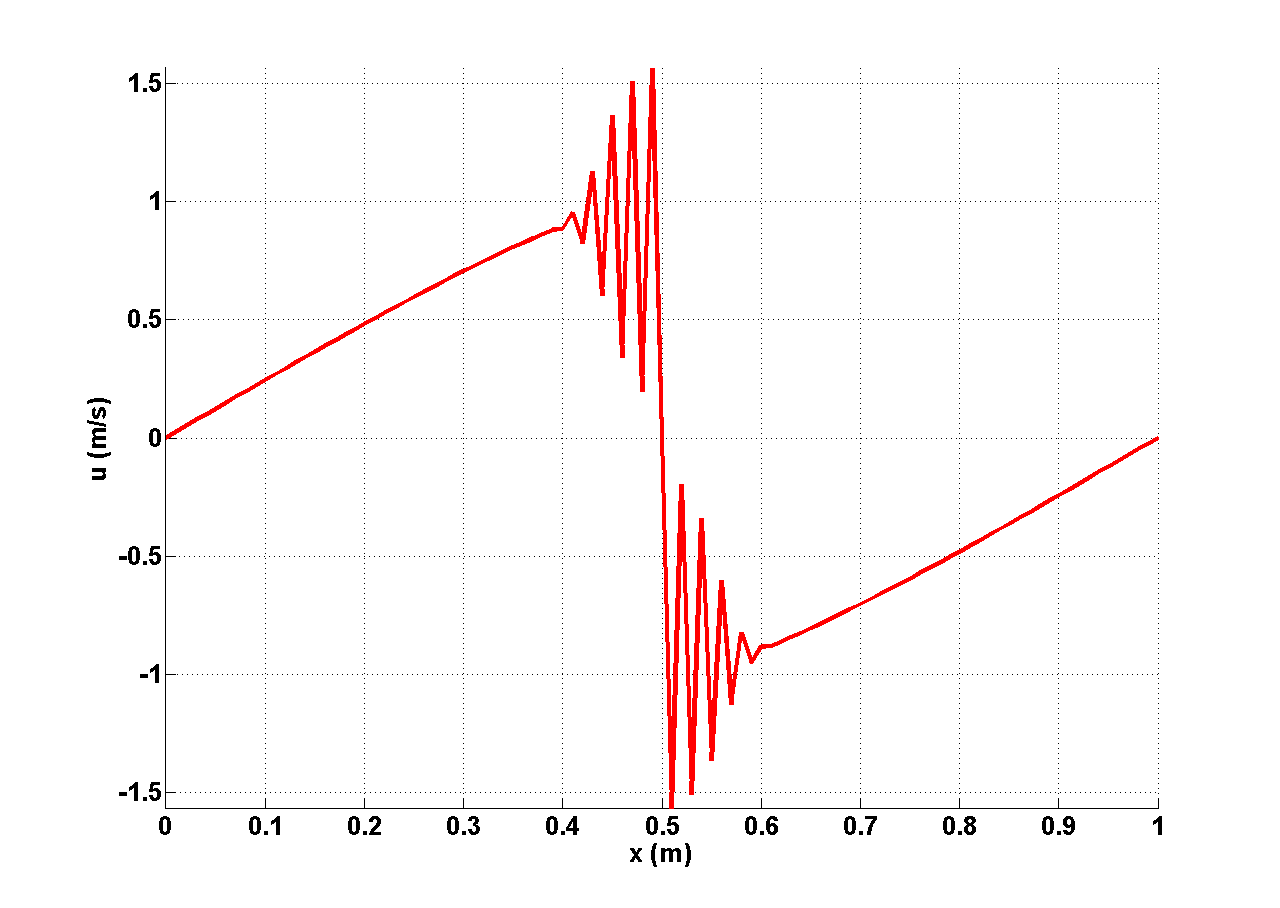
\includegraphics[width=\textwidth]{figures_burgers/1D_sol_free.png}
                %\caption{Without stabilization.}
        %\end{subfigure}%
        %\begin{subfigure}[b]{0.37\textwidth}
                %\centering
                %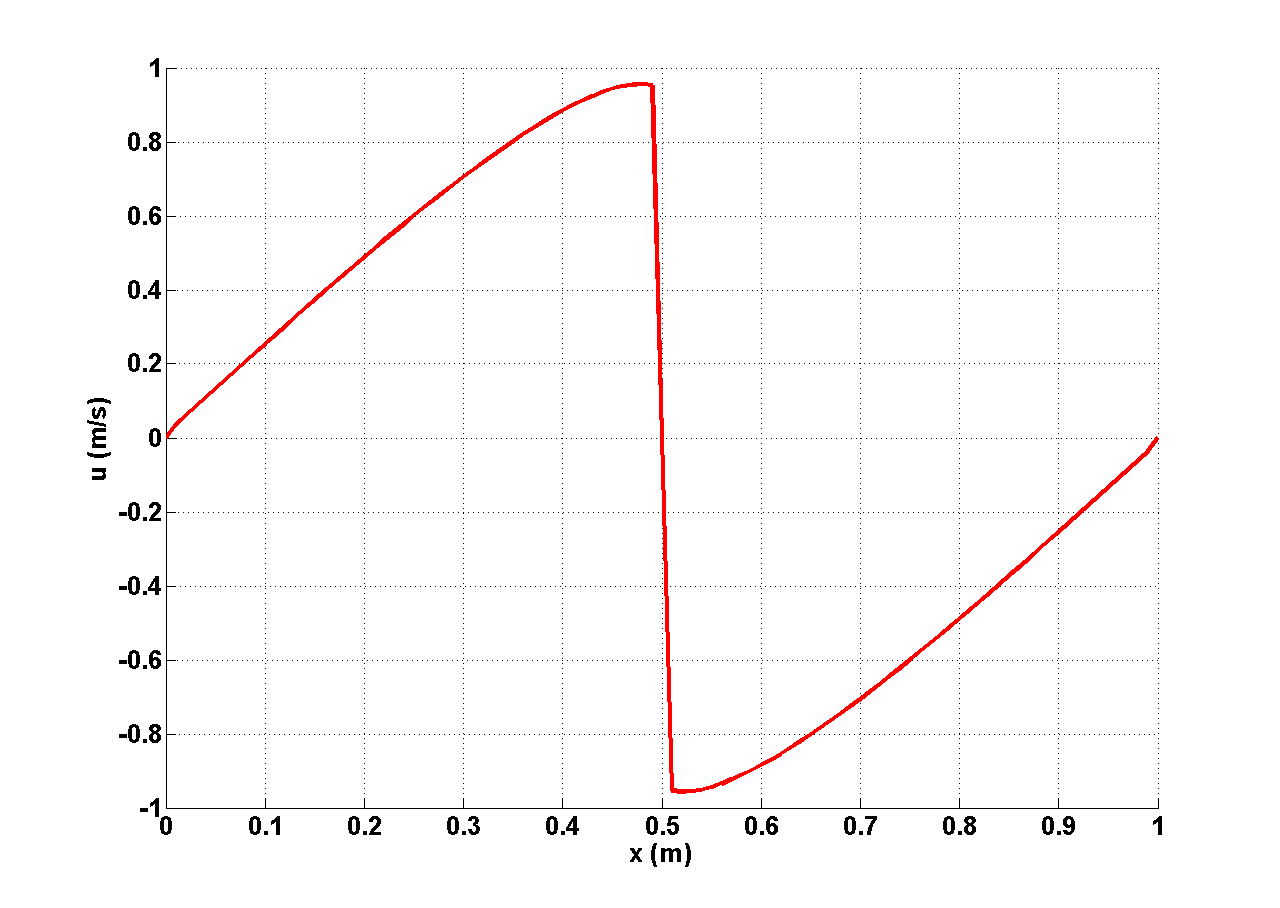
\includegraphics[width=\textwidth]{figures_burgers/1D_sol_fo.png}
                %\caption{With first-order viscosity.}
        %\end{subfigure}
        %
        %\begin{subfigure}[b]{0.37\textwidth}
                %\centering
                %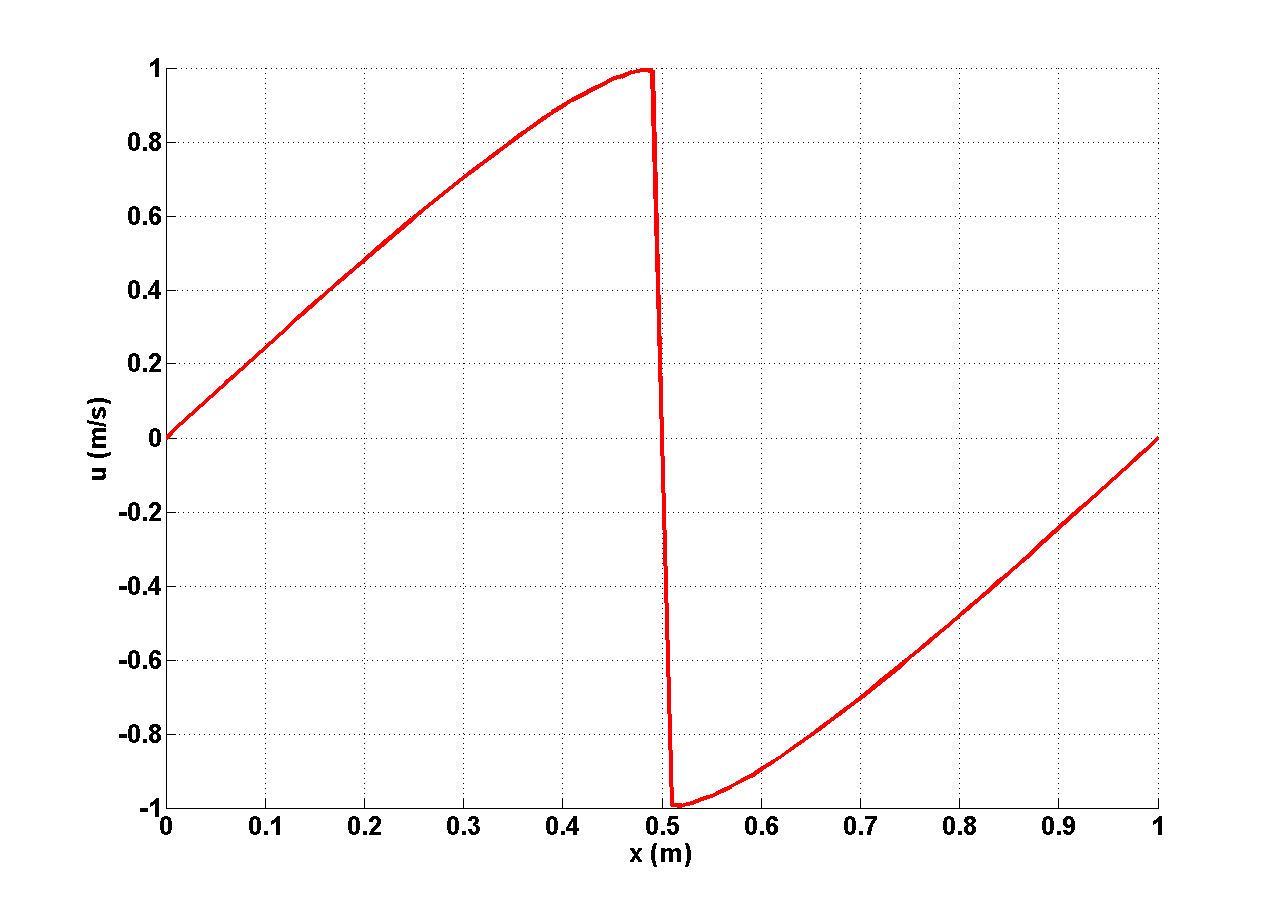
\includegraphics[width=\textwidth]{figures_burgers/1D_sol_ev.png}
                %\caption{With the EVM.}
        %\end{subfigure}
        %\begin{subfigure}[b]{0.37\textwidth}
                %\centering
                %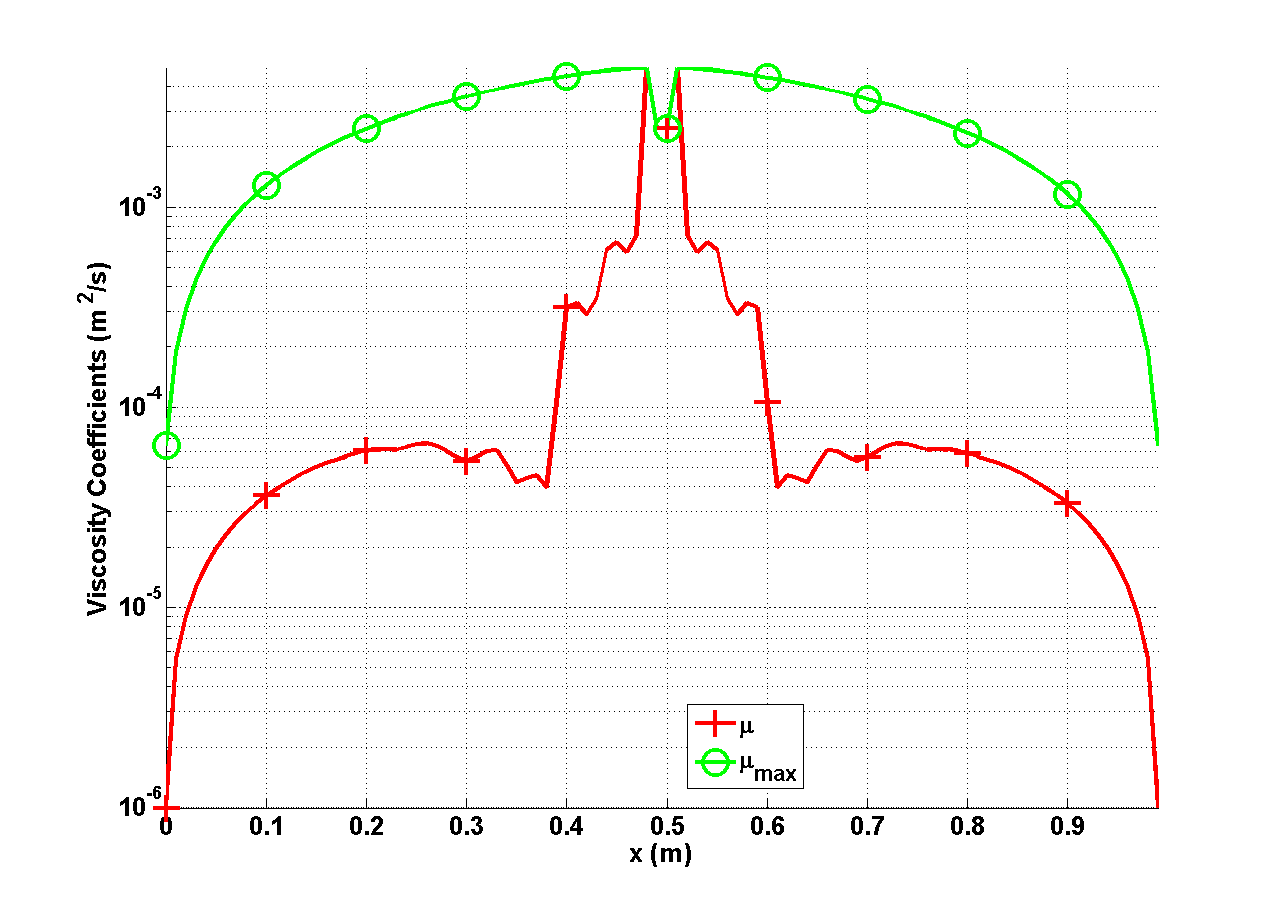
\includegraphics[width=\textwidth]{figures_burgers/1D_visc.png}
                %\caption{Viscosity coefficient profiles.}
        %\end{subfigure}
%\end{figure}
\begin{figure}
\centering
\subfigure[Without stabilization]{
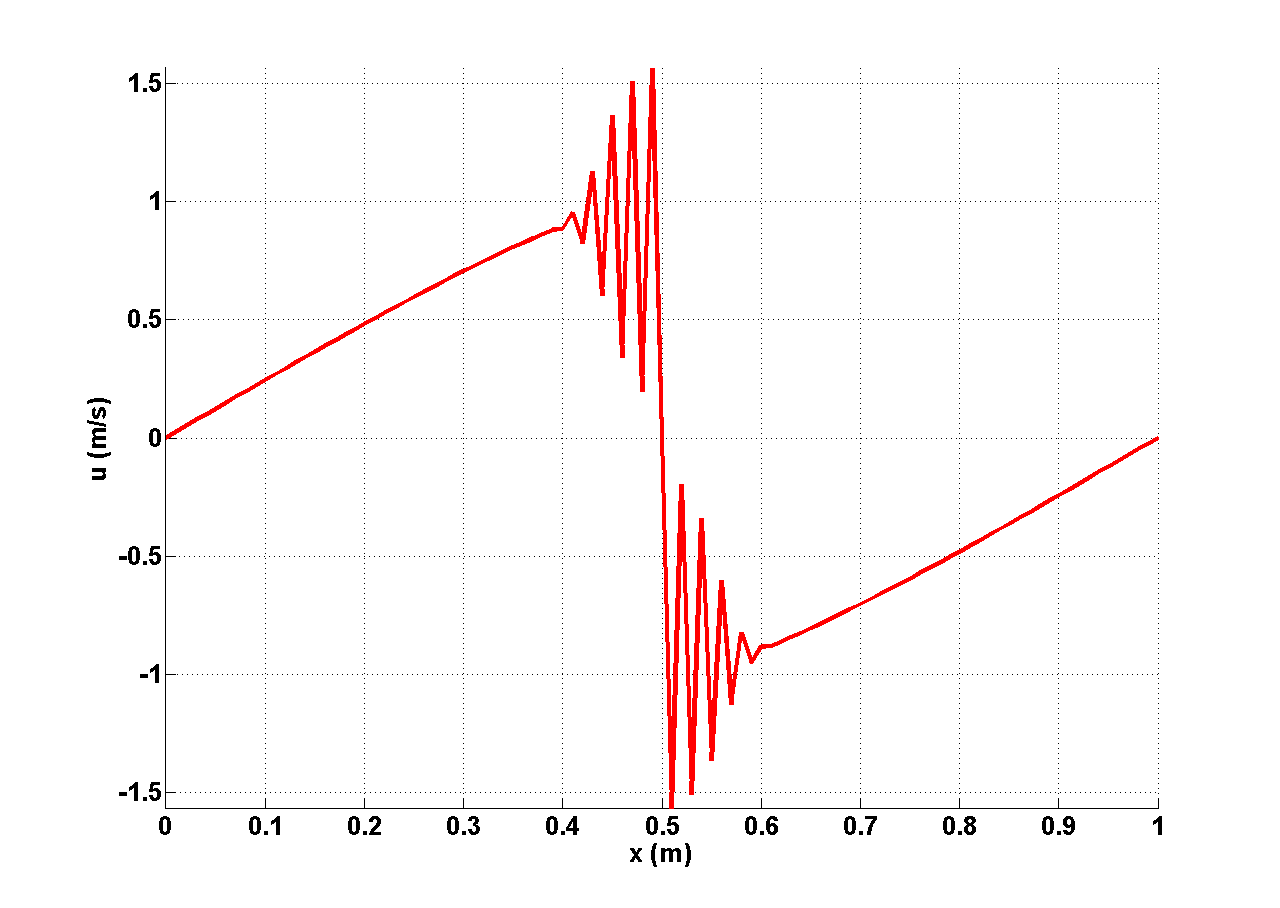
\includegraphics[width=0.4\textwidth]{figures_burgers/1D_sol_free.png}
}
\subfigure[With first-order viscosity]{
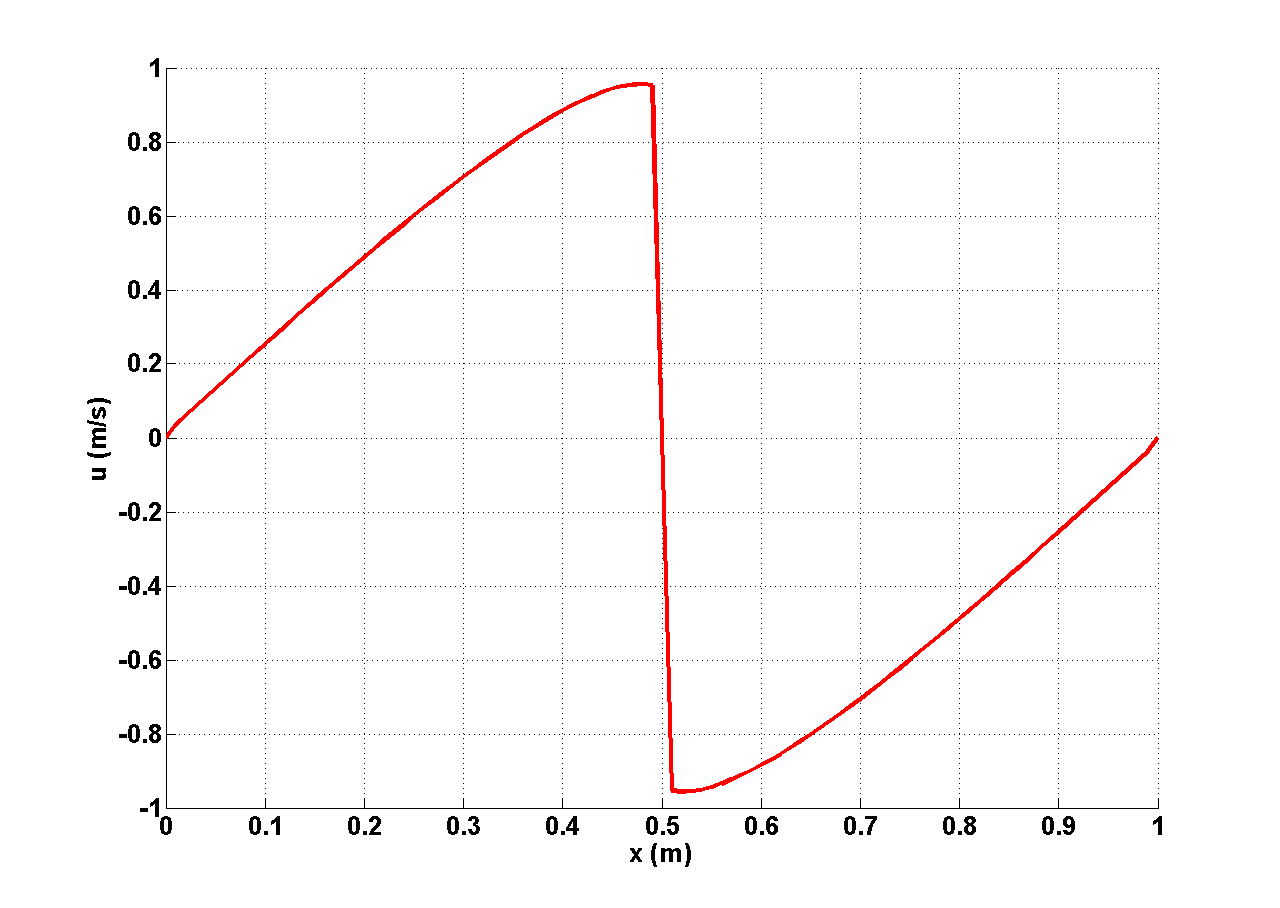
\includegraphics[width=0.4\textwidth]{figures_burgers/1D_sol_fo.png}
}
\subfigure[With entropy viscosity]{
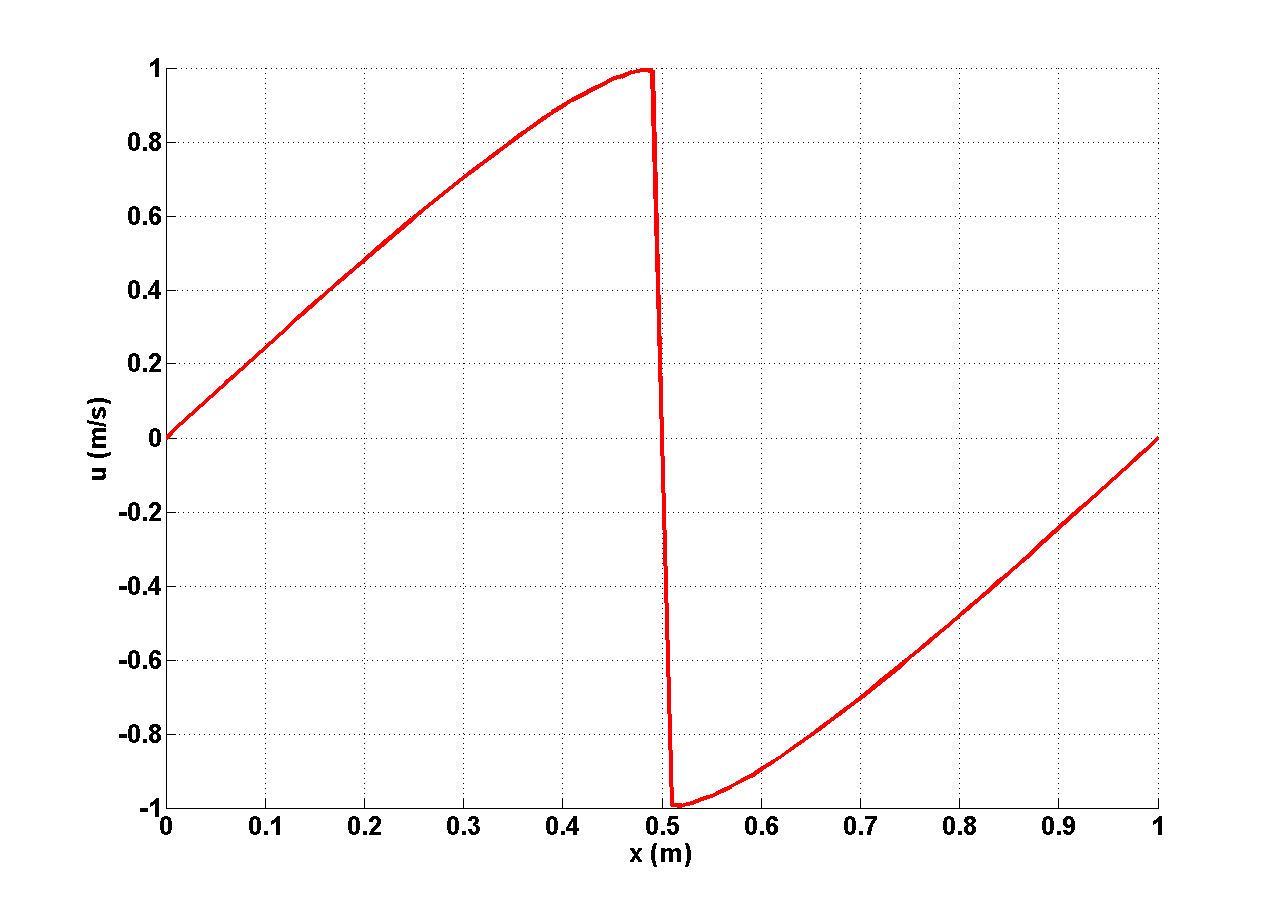
\includegraphics[width=0.4\textwidth]{figures_burgers/1D_sol_ev.png}
}
% \subfigure[Viscosity coefficient profiles \tcr{(log scale !!!)}]{
\subfigure[Viscosity coefficient profiles]{
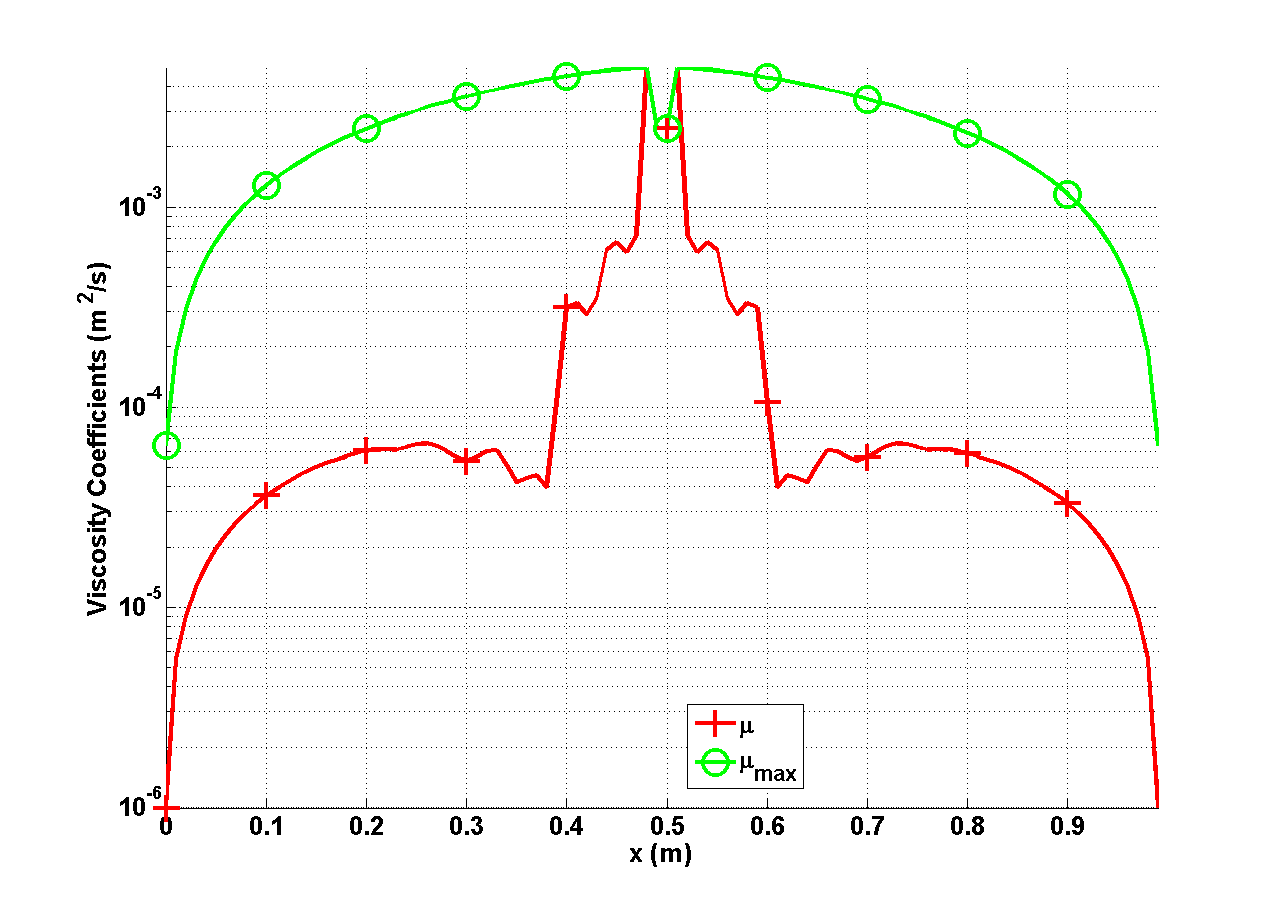
\includegraphics[width=0.4\textwidth]{figures_burgers/1D_visc.png}
}
\end{figure}

\end{frame}
%%%%%%%%%%%%%%%%%%%%%%%%%%%%%%%%%%%%%%%%%%%%%%%%%%%%%%%%%%%%%%%%%%%%

%%%%%%%%%%%%%%%%%%%%%%%%%%%%%%%%%%%%%%%%%%%%%%%%%%%%%%%%%%%%%%%%%%%%
\begin{frame}
\begin{figure}
	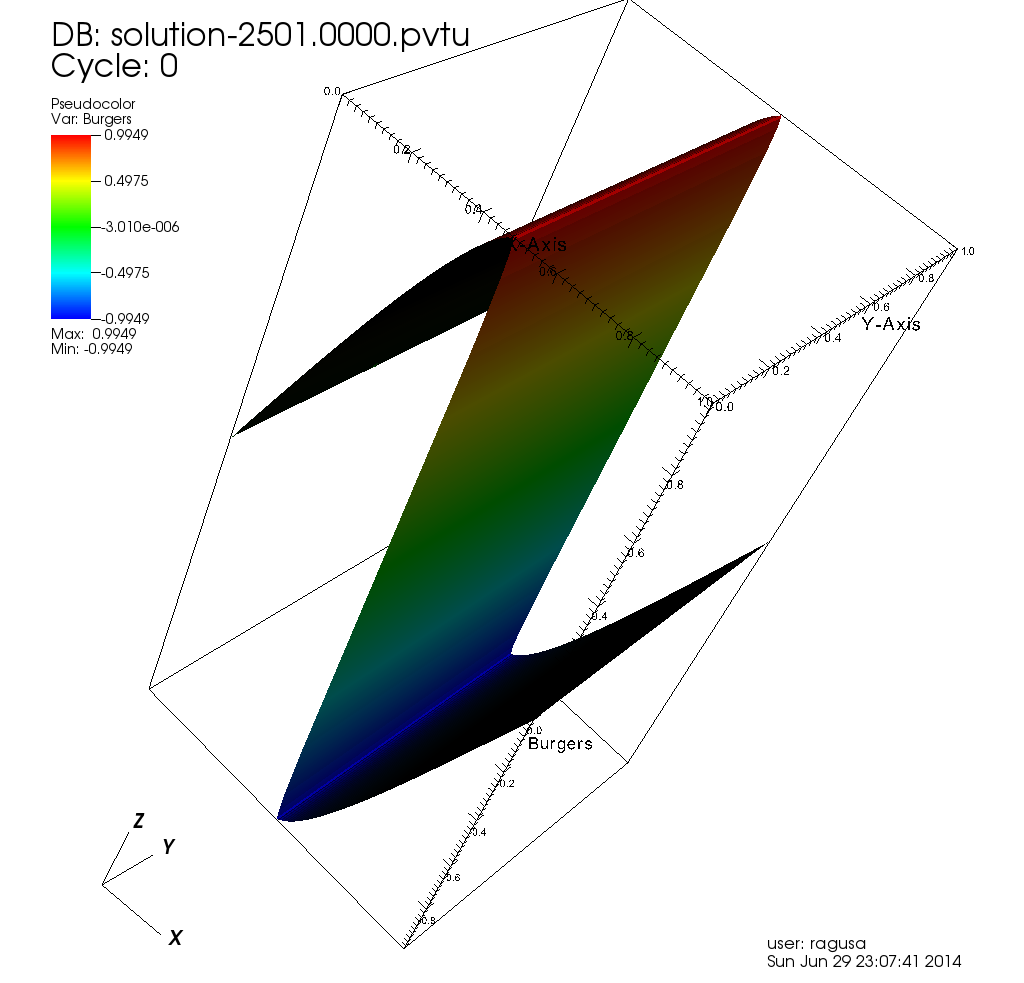
\includegraphics[height=7cm, keepaspectratio=true]{figures_burgers/burgers0000.png}
\end{figure}
\end{frame}
%%%%%%%%%%%%%%%%%%%%%%%%%%%%%%%%%%%%%%%%%%%%%%%%%%%%%%%%%%%%%%%%%%%%

%%%%%%%%%%%%%%%%%%%%%%%%%%%%%%%%%%%%%%%%%%%%%%%%%%%%%%%%%%%%%%%%%%%%%
%\begin{frame} 
%\begin{figure}
%	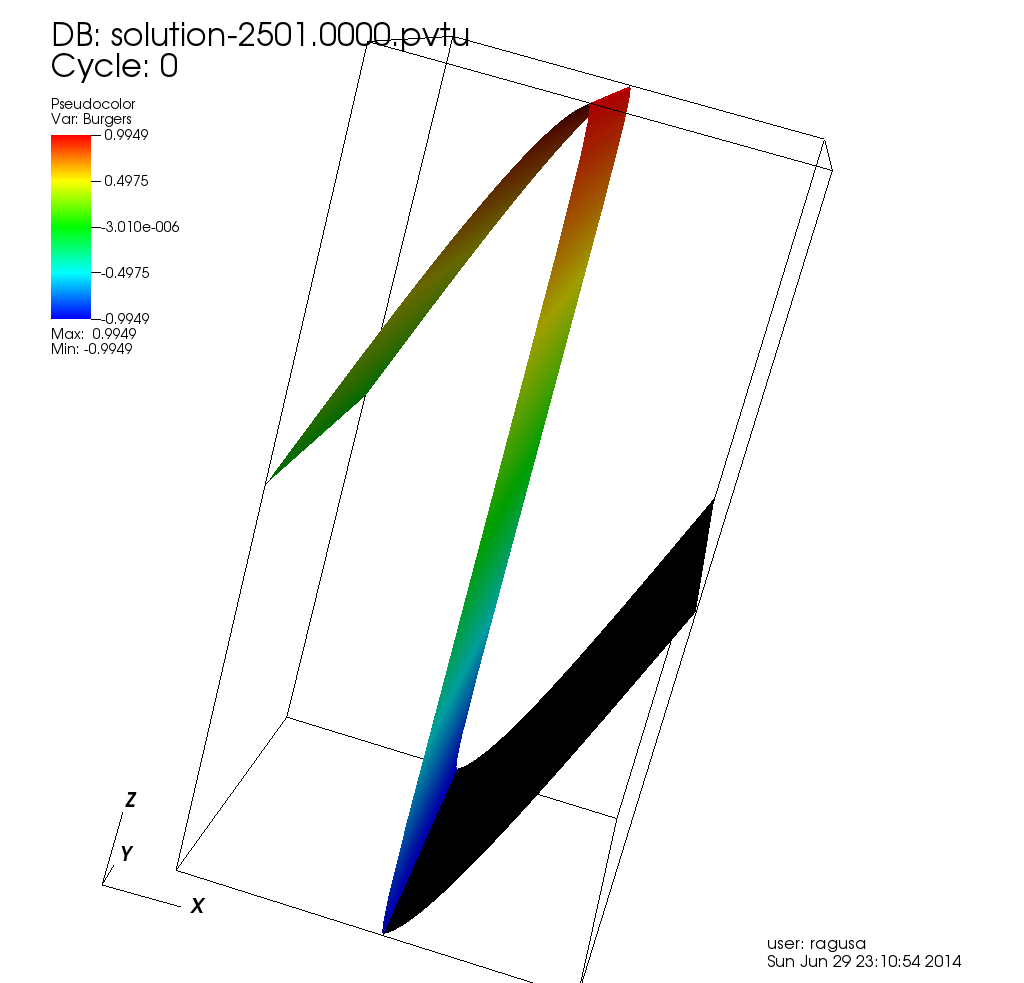
\includegraphics[height=7cm, keepaspectratio=true]{figures_burgers/burgers20000.png}
%\end{figure}
%\end{frame}
%%%%%%%%%%%%%%%%%%%%%%%%%%%%%%%%%%%%%%%%%%%%%%%%%%%%%%%%%%%%%%%%%%%%%

%%%%%%%%%%%%%%%%%%%%%%%%%%%%%%%%%%%%%%%%%%%%%%%%%%%%%%%%%%%%%%%%%%%%
%\subsection{Application to the Entropy Viscosity Method to the Euler Equations}
%%%%%%%%%%%%%%%%%%%%%%%%%%%%%%%%%%%%%%%%%%%%%%%%%%%%%%%%%%%%%%%%%%%%

%%%%%%%%%%%%%%%%%%%%%%%%%%%%%%%%%%%%%%%%%%%%%%%%%%%%%%%%%%%%%%%%%%%%
%************************************************
%\subsection{Entropy-viscosity method: original supersonic formulation}
%%************************************************

%%%%%%%%%%%%%%%%%%%%%%%%%%%%%%%%%%%%%%%%%%%%%%%%%%%%%%%%%%%%%%%%%%%%
\begin{frame}{Viscous regularization of Euler equations}

\begin{block}{\tcr{Regularized} Euler equations}
\begin{subequations}
\label{eq:euler_visc}
%
\begin{equation}
\partial_t \rho + \div \left( \rho \vec{u} \right) = \textcolor{red}{\div \vec{f}} \nonumber
\end{equation}
%
\begin{equation}
\partial_t \left( \rho \vec{u} \right) + \div \left( \rho \vec{u} \otimes \vec{u} + P \mathbb{I} \right) =  \textcolor{red}{\div \mathbb{g} }\nonumber
\end{equation}
%
\begin{equation}
\partial_t \left( \rho E  \right) + \div \left[ \vec{u} \left( \rho E + P \right) \right] = \textcolor{red}{\div \vec{h} }\nonumber
\end{equation}
\end{subequations}

\smallskip

How to select the \tcr{artificial viscous fluxes}?

\smallskip

By proving that the \tcr{regularized} equations satisfy a minimum principle on the specific entropy, \tcr{$s(\rho,e)$}  \tcb{[Guermond/Popov/Pasquetti (JCP 2011)]}

\end{block}

\begin{block}{Minimum entropy principle}
\be
\inf_{x\in \mathbb{R}^d} s(x,t) \ge \inf_{x\in \mathbb{R}^d} s_0(x) \qquad \forall t \ge 0
\ee
\end{block}

\end{frame}
%%%%%%%%%%%%%%%%%%%%%%%%%%%%%%%%%%%%%%%%%%%%%%%%%%%%%%%%%%%%%%%%%%%%


%%%%%%%%%%%%%%%%%%%%%%%%%%%%%%%%%%%%%%%%%%%%%%%%%%%%%%%%%%%%%%%%%%%%
\begin{frame}{General idea of the derivation}
%
\vspace{-1mm}
\begin{block}{Goal: To obtain an entropy relationship: $\rho ( \partial_t s + \vec{u} \cdot \grad s ) = \ldots  \tcr{\ge 0}$}
Entropy is a function of density $\rho$ and internal energy $e$. Using chain rule, we have
\[
\partial_\alpha s = s_\rho \tcr{\partial_\alpha \rho} + s_e \tcr{\partial_\alpha e} \quad \text{ with } \alpha={t,x}
\]
Now, re-write Euler equations in non-conservative form as a function of $\rho$, $u$, and $e$.
\end{block}
%
\vspace{-1mm}
\begin{block}{Entropy equation}
%Use chain rule and the mass and internal energy equations to get:
The following choice of viscous fluxes, $\vec{f} = \kappa \grad \rho$, $\mathbb{g} = \mu \rho \grad^s \vec{u} + \vec{u}\otimes \vec{f}$,and $\vec{h} = \kappa \grad(\rho e) -\tfrac{1}{2}u^2 \vec{f} + \mathbb{g}\cdot \vec{u}$, yields:
\begin{equation}
\rho \left( \partial_t s + \mbold{u} \cdot \grad s \right) = 
\div \left( \rho \kappa \grad s \right) -  \kappa \rho \mathbf{Q} +  s_e \mu \grad^s \mbold{u} : \grad \mbold{u}\nonumber
\end{equation}
\end{block}
%
\vspace{-1mm}
\begin{block}{Quadratic form}
\begin{equation}
\mathbf{Q} = X^t \mathbb{\Sigma} X 
\quad \text{ with } 
X = 
\begin{bmatrix}
\grad \rho \\
\grad e 
\end{bmatrix}
\text{ and } 
\mathbb{\Sigma} = 
\begin{bmatrix}
       \partial_{\rho} (\rho^2 \partial_{\rho} s) & \partial_{\rho,e} s  \\[0.3em]
       \partial_{\rho,e} s & \partial_{e,e} s           \\[0.3em]
\end{bmatrix} \nonumber 
\end{equation}
The form $\mathbf{Q}$ is negative definite if and only if $-s$ is convex with respect to $e$ and $\rho^{-1}$.
\end{block}
%
\vspace{-1mm}
\tcr{QED}  \ \ (recall: $s_e = 1/T > 0 $)

\end{frame}
%%%%%%%%%%%%%%%%%%%%%%%%%%%%%%%%%%%%%%%%%%%%%%%%%%%%%%%%%%%%%%%%%%%%

%\end{document}
%%%%%%%%%%%%%%%%%%%%%%%%%%%%%%%%%%%%%%%%%%%%%%%%%%%%%%%%%%%%%%%%%%%%
\begin{frame}
\begin{block}{Euler equations with viscous regularization (final form)}
\begin{subequations}
%
%\text{Continuity equation:}
\begin{equation}
\partial_t \rho + \div \left( \rho \vec{u} \right) = \textcolor{red}{\div \left( \kappa  \grad \rho \right)} \nonumber
\end{equation}
%
%\text{Momentum equation:}
\begin{equation}
\partial_t \left( \rho \vec{u} \right) + \div \left( \rho \vec{u} \otimes \vec{u} + P \mathbb{I} \right) =  \textcolor{red}{\div \left( \mu \rho  \grad^s \vec{u}  + \kappa \vec{u} \otimes \grad \rho \right) }\nonumber
\end{equation}
%
%\text{Energy equation:}
\begin{equation}
\partial_t \left( \rho E  \right) + \div \left[ \vec{u} \left( \rho E + P \right) \right] = \textcolor{red}{\div \left( \kappa \grad \left( \rho e \right) + \frac{1}{2}|| \vec{u} ||^2 \kappa \grad \rho +  \rho \mu \vec{u} \grad \vec{u}  \right) }\nonumber
\end{equation}
\end{subequations}

\smallskip

where $\kappa$ and $\mu$ are positive viscosity coefficients.
\end{block}

\begin{block}{Definition of the viscosity coefficients}
\begin{itemize}
\item As before, $\mu = \min(\mu^{LLF}, \mu^{\textit{entr}})$ and $\kappa = \min (\kappa^{LLF}, \kappa^{\textit{entr}})$ 
\item Entropy viscosities \tcr{$\propto$ entropy production}
\item All-speed (from low-Mach to supersonic) extension by \tcb{Delchini/Ragusa/Berry in Computers \& Fluids, 2015} 
%%\item
%%Note that if $\mu = \kappa$ (and one selects $\grad \vec{u} $ instead of $\grad^s \vec{u} $), we recover a parabolic regularization (on $\rho$, $\rho \vec{u}$, and $\rho E$).
\end{itemize}
\end{block}

%\begin{block}{}
%\hspace{0.5cm} $\bullet$ Multi-wave problem: $\lambda_1 = \vec{u} \cdot \vec{n} - c $, $\lambda_2 = \vec{u} \cdot \vec{n} + c $ and $\lambda_{3, \dots, 3+D} = \vec{u} \cdot \vec{n}$. \\
%\hspace{0.5cm} $\bullet$ $\kappa$ and $\mu$ are two positive viscosity coefficients.
%\end{block}
\end{frame}
%%%%%%%%%%%%%%%%%%%%%%%%%%%%%%%%%%%%%%%%%%%%%%%%%%%%%%%%%%%%%%%%%%%%

%%%%%%%%%%%%%%%%%%%%%%%%%%%%%%%%%%%%%%%%%%%%%%%%%%%%%%%%%%%%%%%%%%%%%
\begin{frame}{Leblanc shock tube}
\setcounter{subfigure}{0}% Reset subfigure counter
\vspace{-2mm}
\begin{figure}[H]
\centering
\subfigure[Density]{
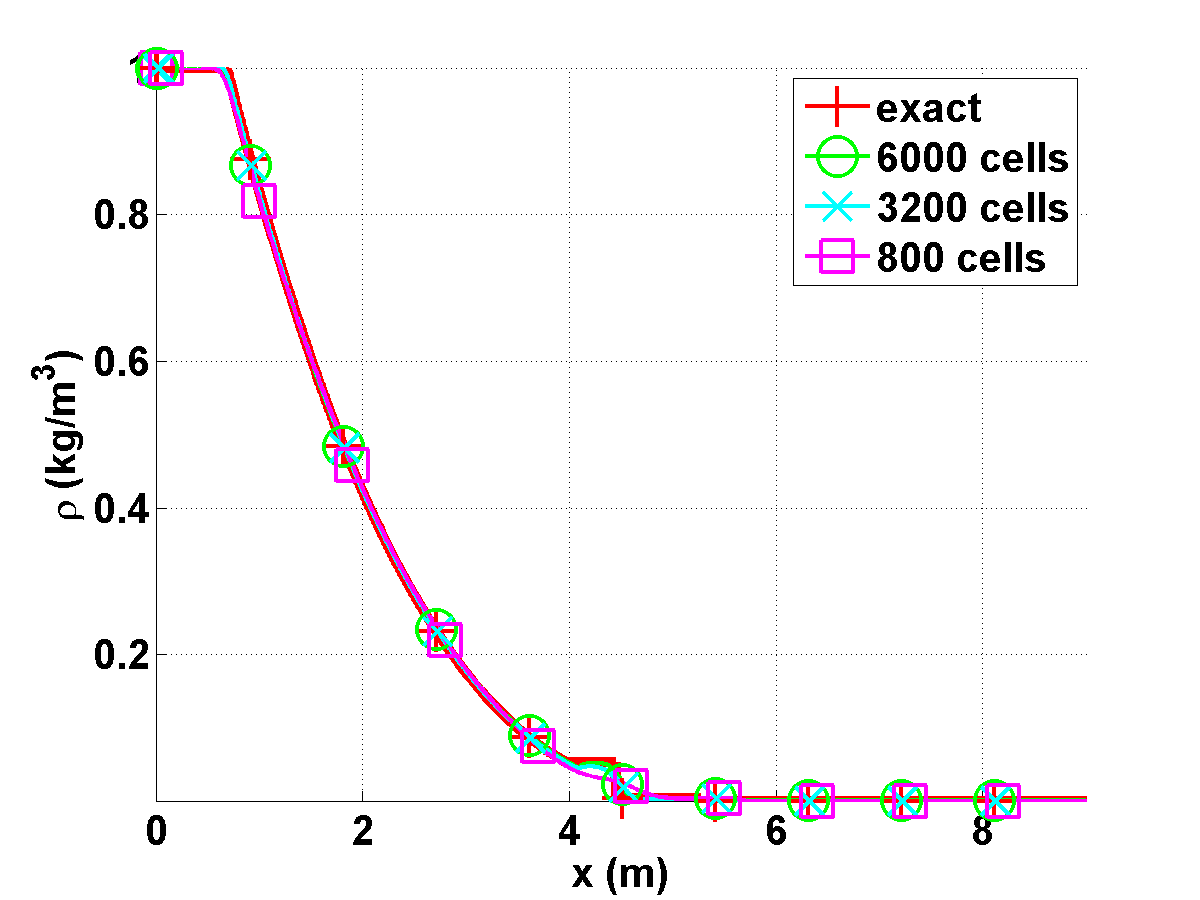
\includegraphics[width=0.4\textwidth]{figures_leblanc/Leblanc_exact_and_numerical_stt_density_6000.png}
}
\subfigure[Momentum]{
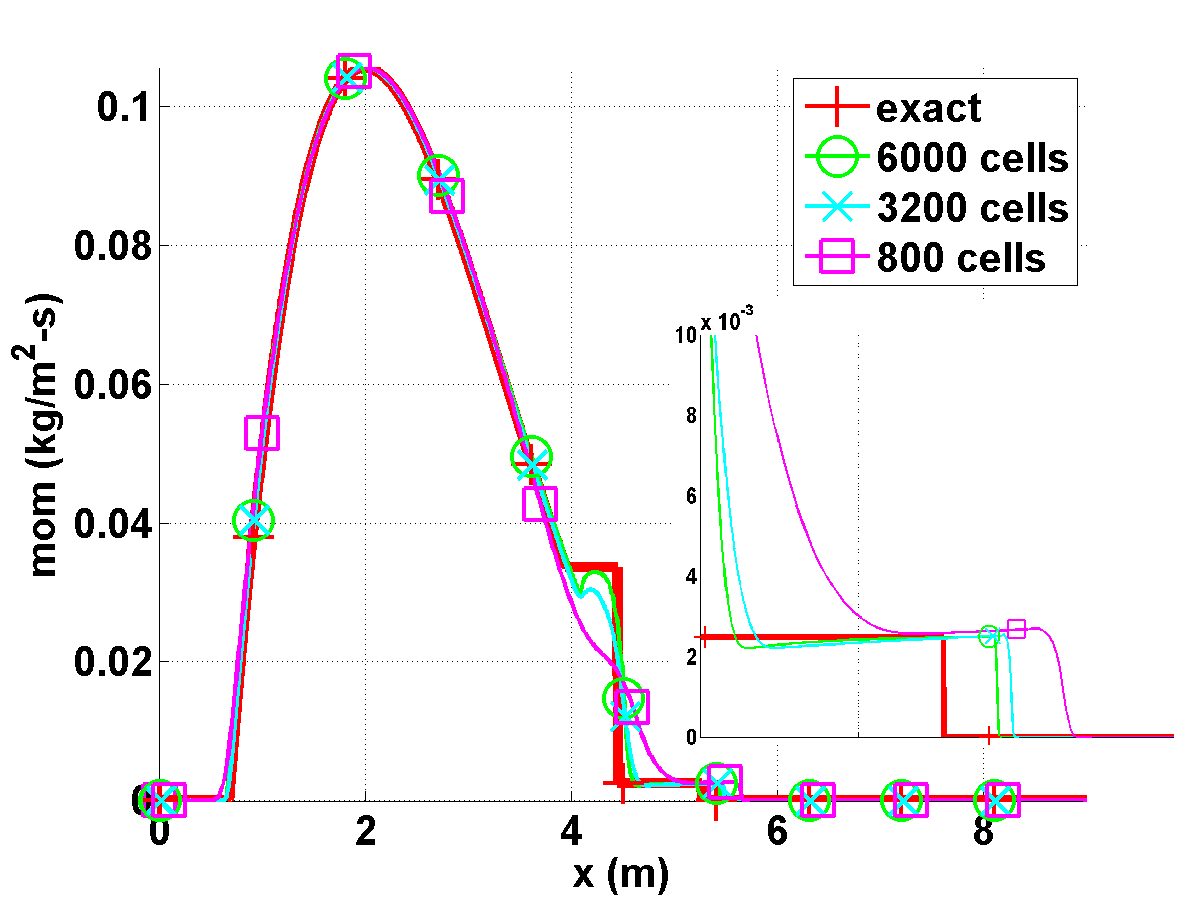
\includegraphics[width=0.4\textwidth]{figures_leblanc/Leblanc_exact_and_numerical_stt_momentum_6000.png}
}
\subfigure[Total energy]{
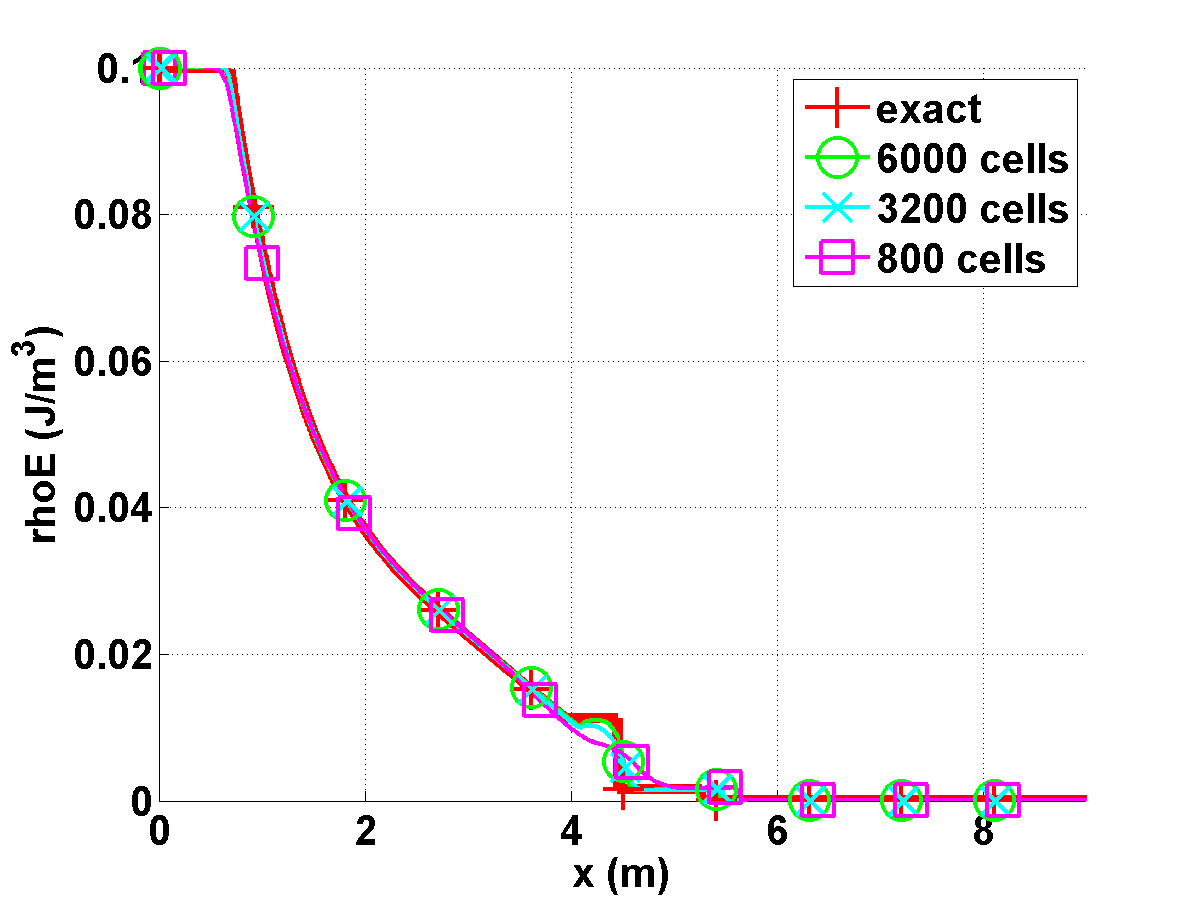
\includegraphics[width=0.4\textwidth]{figures_leblanc/Leblanc_exact_and_numerical_stt_total_energy_6000.png}
}
\subfigure[Viscosity]{
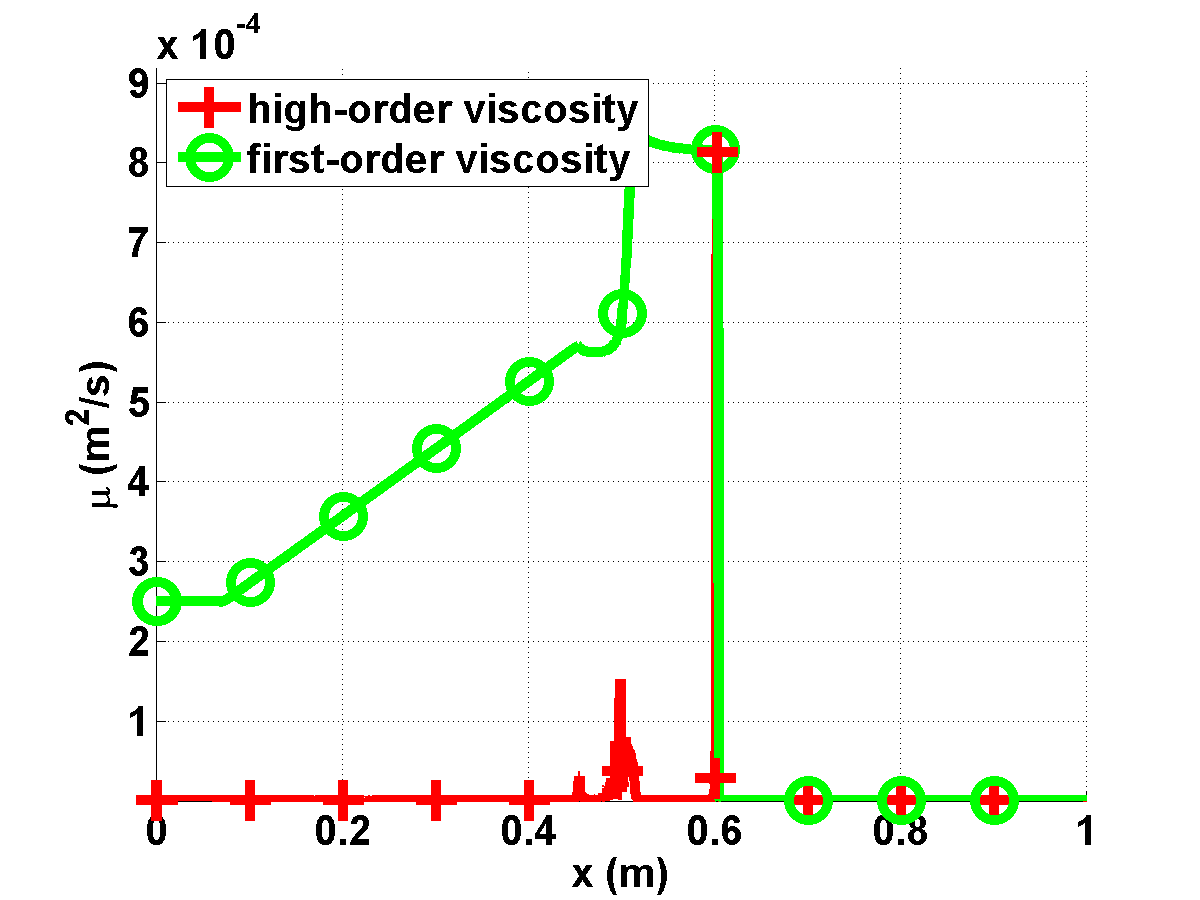
\includegraphics[width=0.4\textwidth]{figures_leblanc/Leblanc_viscosity_numerical_6000.png}
}
\end{figure}
\end{frame}
%%%%%%%%%%%%%%%%%%%%%%%%%%%%%%%%%%%%%%%%%%%%%%%%%%%%%%%%%%%%%%%%%%%%%

%%%%%%%%%%%%%%%%%%%%%%%%%%%%%%%%%%%%%%%%%%%%%%%%%%%%%%%%%%%%%%%%%%%%%
\begin{frame}{2-D explosion test}
\setcounter{subfigure}{0}% Reset subfigure counter
\begin{figure}[H]
\centering
\subfigure[Density]{
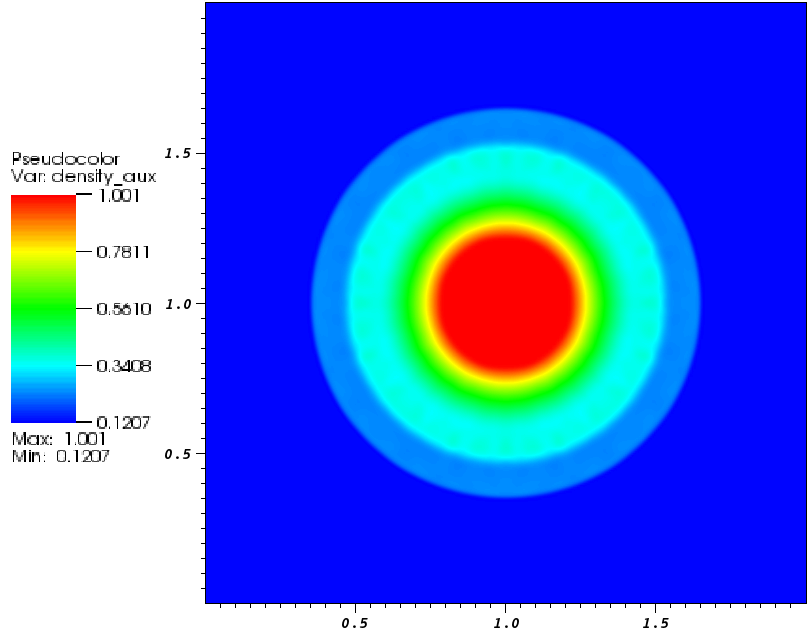
\includegraphics[width=0.48\textwidth]{figures_more_euler/Explosion_density_profiles.png}
}
\subfigure[Viscosity]{
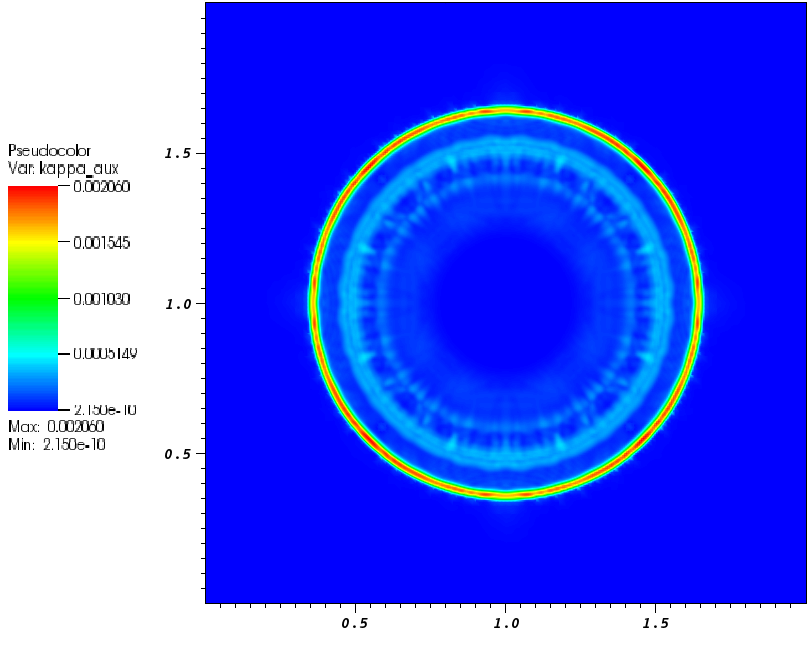
\includegraphics[width=0.48\textwidth]{figures_more_euler/Explosion_viscosity_profiles.png}
}
\end{figure}
\end{frame}
%%%%%%%%%%%%%%%%%%%%%%%%%%%%%%%%%%%%%%%%%%%%%%%%%%%%%%%%%%%%%%%%%%%%%

%%%%%%%%%%%%%%%%%%%%%%%%%%%%%%%%%%%%%%%%%%%%%%%%%%%%%%%%%%%%%%%%%%%%%
%\begin{frame}{Euler example: Mach-3 forward facing step}
%
%\begin{center}
%\movie[width=6cm,height=4cm,showcontrols=true,externalviewer]{
\includegraphics[width=6cm,height=4cm]{engr.pdf}}{movs/forward_facing_step_density_movie.mpeg}\\
%\end{center}
%
%\begin{center}
%\begin{columns}
%\column{.5\textwidth}
%\includemedia[addresource=compression_corner.mp4, activate=pageopen, deactivate=pageclose, width=6.5cm, height=5cm, flashvars={source=mov/compression_corner.mp4 & autoPlay=true & loop=true }]{}{VPlayer.swf}
%\column{.5\textwidth}
%\includemedia[addresource=compression_corner_viscosity.mp4, activate=pageopen, deactivate=pageclose, width=6.5cm, height=5cm, flashvars={source=mov/compression_corner_viscosity.mp4 & autoPlay=true & loop=true }]{}{VPlayer.swf}
%\end{columns}
%\end{center}
%
%
%\end{frame}
%%%%%%%%%%%%%%%%%%%%%%%%%%%%%%%%%%%%%%%%%%%%%%%%%%%%%%%%%%%%%%%%%%%%%
%
%%%%%%%%%%%%%%%%%%%%%%%%%%%%%%%%%%%%%%%%%%%%%%%%%%%%%%%%%%%%%%%%%%%%%
%\begin{frame}{Mach-3 forward facing step: density contour}
%
%\begin{center}
%\movie[width=6cm,height=4cm,showcontrols=true,externalviewer]{
\includegraphics[width=6cm,height=4cm]{engr.pdf}}{movs/forward_facing_step_density_movie.mpeg}\\
%\end{center}
%
%\end{frame}
%%%%%%%%%%%%%%%%%%%%%%%%%%%%%%%%%%%%%%%%%%%%%%%%%%%%%%%%%%%%%%%%%%%%%
%
%%%%%%%%%%%%%%%%%%%%%%%%%%%%%%%%%%%%%%%%%%%%%%%%%%%%%%%%%%%%%%%%%%%%%
%\begin{frame}{Mach-3 forward facing step: viscosity contour}
%
%\begin{center}
%\movie[width=6cm,height=4cm,showcontrols=true,externalviewer]{
\includegraphics[width=6cm,height=4cm]{engr.pdf}}{movs/forward_facing_step_viscosity.mpeg}\\
%\end{center}
%
%\end{frame}
%%%%%%%%%%%%%%%%%%%%%%%%%%%%%%%%%%%%%%%%%%%%%%%%%%%%%%%%%%%%%%%%%%%%%
%
%%%%%%%%%%%%%%%%%%%%%%%%%%%%%%%%%%%%%%%%%%%%%%%%%%%%%%%%%%%%%%%%%%%%
%%%%%%%%%%%%%%%%%%%%%%%%%%%%%%%%%%%%%%%%%%%%%%%%%%%%%%%%%%%%%%%%%%%%
\section{Development of entropy-based artificial viscosity for the GRHD}
%%%%%%%%%%%%%%%%%%%%%%%%%%%%%%%%%%%%%%%%%%%%%%%%%%%%%%%%%%%%%%%%%%%%
%%%%%%%%%%%%%%%%%%%%%%%%%%%%%%%%%%%%%%%%%%%%%%%%%%%%%%%%%%%%%%%%%%%%

%%%%%%%%%%%%%%%%%%%%%%%%%%%%%%%%%%%%%%%%%%%%%%%%%%%%%%%%%%%%%%%%%%%%
\subsection{Questions to answer}
%%%%%%%%%%%%%%%%%%%%%%%%%%%%%%%%%%%%%%%%%%%%%%%%%%%%%%%%%%%%%%%%%%%%

%%%%%%%%%%%%%%%%%%%%%%%%%%%%%%%%%%%%%%%%%%%%%%%%%%%%%%%%%%%%%%%%%%%%
\begin{frame}{Entropy-based artificial viscosity technique for the GRHD}
\vspace{-2mm}
\begin{block}{Questions to answer:}
\begin{enumerate}
\item 
The GRHD equations are \tcr{not hyperbolic}. Can we apply the entropy viscosity method (EVM)?
\begin{itemize}
\item Our initial attempt: apply the EVM to the hyperbolic part of the GRHD [an idea similar to \tcb{Balsara JQSRT 1999}, \tcb{Lowrie\&Morel JQSRT 2001}]
\end{itemize}
\item
What is an appropriate functional form for the entropy of the GRHD, $\tcr{s(\rho,e,\epsilon) = \ldots}$\tcr{???} 
\item
What is an appropriate expression for the viscous fluxes so that the \tcr{regularized} GRHD eqs satisfy 
the minimum entropy principle?
\item
Is the viscous regularization well-behaved in the \tcr{equilibrium-diffusion limit}?
\end{enumerate}
\end{block}
\vspace{-4mm}
\begin{columns}
    \begin{column}{0.7\textwidth}

\begin{block}{Hyperbolic part of the GRHD}
%[an idea similar to \tcb{Balsara JQSRT 1999}, \tcb{Lowrie\&Morel JQSRT 2001}]
\begin{subequations}
\begin{equation}
\partial_t \left( \rho \right) + \partial_x\left( \rho u \right) = 0 
\end{equation}
%
\begin{equation}
\partial_t \left( \rho u\right) + \partial_x \left(\rho u^2 + P + \frac{\epsilon}{3} \right) = 0 
\end{equation}
%
\begin{equation}
\partial_t \left( \rho E\right) + \partial_x \left[ u \left( \rho E + P \right) \right] +\frac{u}{3} \partial_x \epsilon = 0
\end{equation}
%
\begin{equation}
\partial_t \epsilon + \frac{4}{3} \partial_x \left( u \epsilon \right) - \frac{u}{3} \partial_x \epsilon = 0
\end{equation}
\end{subequations}
\end{block}

    \end{column}
    \begin{column}{0.3\textwidth}

        \begin{block}{Eigenvalues}
\begin{align*}
\lambda_{1,4} &= u\pm c_m \\
\lambda_{2,3} &= u     
\end{align*}
with
\begin{equation*}
c_m^2 = \underbrace{P_{\rho} + \frac{P}{\rho^2}P_e}_{c_{Euler}^2} + \underbrace{\frac{4 \epsilon}{9\rho}}_{c^2_{rad}} 
\end{equation*}
        \end{block}

    \end{column}
\end{columns}

\end{frame}
%%%%%%%%%%%%%%%%%%%%%%%%%%%%%%%%%%%%%%%%%%%%%%%%%%%%%%%%%%%%%%%%%%%%

%%%%%%%%%%%%%%%%%%%%%%%%%%%%%%%%%%%%%%%%%%%%%%%%%%%%%%%%%%%%%%%%%%%%
\subsection{Previous results (JCP 2015)}
%%%%%%%%%%%%%%%%%%%%%%%%%%%%%%%%%%%%%%%%%%%%%%%%%%%%%%%%%%%%%%%%%%%%


%%%%%%%%%%%%%%%%%%%%%%%%%%%%%%%%%%%%%%%%%%%%%%%%%%%%%%%%%%%%%%%%%%%%
\begin{frame}{Entropy-based artificial viscosity for the GRHD: derivation}

\begin{block}{Study of the hyperbolic parts of the GRHD: process}
\begin{enumerate}
\item Add viscous regularization (fluxes) to the equations
\begin{subequations}
\begin{equation}
\partial_t \left( \rho \right) + \partial_x\left( \rho u \right) = \tcr{\partial_x f}
\end{equation}
%
\begin{equation}
\partial_t \left( \rho u\right) + \partial_x \left(\rho u^2 + P + \frac{\epsilon}{3} \right) = \tcr{\partial_x g }
\end{equation}
%
\begin{equation}
\partial_t \left( \rho E\right) + \partial_x \left[ u \left( \rho E + P \right) \right] +\frac{u}{3} \partial_x \epsilon = \tcr{\partial_x h  }
\end{equation}
%
\begin{equation}
\partial_t \epsilon + \frac{4}{3} \partial_x \left( u \epsilon \right) - \frac{u}{3} \partial_x \epsilon = \tcr{\partial_x \ell}
\end{equation}
\end{subequations}
\item With \tcr{$s(\rho,e,\epsilon)$}, use chain rule to obtain the entropy relationship
	\begin{equation}
		\partial_{\alpha} s = \partial_{\rho} s \partial_{\alpha} \rho +  \partial_{e} s \partial_{\alpha}e +  
		\partial_{\epsilon} s \partial_{\alpha} \epsilon 
	\end{equation} 
\item An observation: we can greatly simplify the expression by assuming \tcr{$s(\rho,e,\epsilon) = s_{Euler}(\rho,e) + s_{rad}(\rho,\epsilon)$}
%Use the viscous fluxes obtained for Euler's equations in the material equations (with $\kappa=\mu$), supplemented by an radiation energy viscous flux $\kappa \grad \epsilon$ 
\end{enumerate}
\end{block}

\end{frame}
%%%%%%%%%%%%%%%%%%%%%%%%%%%%%%%%%%%%%%%%%%%%%%%%%%%%%%%%%%%%%%%%%%%%

%%%%%%%%%%%%%%%%%%%%%%%%%%%%%%%%%%%%%%%%%%%%%%%%%%%%%%%%%%%%%%%%%%%%
\begin{frame}
\vspace{-2mm}
\begin{block}{Study of the hyperbolic parts of the GRHD: results}
\begin{enumerate}
\item
%After some tedious algebra, the following form of the entropy $s(\rho,e,\epsilon)$ is obtained
\begin{equation}
s(\rho, e, \epsilon) = s_{Euler}(\rho,e) + \frac{4 a^{1/4}}{3\rho} \epsilon^{\frac{3}{4}}
\end{equation}
\item Using the Eulerian viscous fluxes, supplemented by an radiation energy viscous flux 
%$\vec{\ell}=\kappa \grad \epsilon$  
\begin{equation}
\left\{
 \begin{array}{cl}
  f  &= \kappa \partial_x \rho \\
  g  &= \rho \mu \partial_x u + uf \\
  h  &= \kappa \partial_x (\rho e) - \tfrac{1}{2} u^2 f + g u\\
\ell &= \kappa \partial_x \epsilon
 \end{array}
\right. 
\end{equation}
we get the following result:
\item Entropy conservation statement:
\begin{equation*}
\boxed{
\rho \frac{Ds}{Dt} = 
\partial_x \left( \rho \kappa \partial_x s \right) 
+ (\kappa \partial_x \rho) (\partial_x s )
- \rho \kappa X^T A X
+ s_e \rho \mu (\partial_x u)^2
\ \tcr{ \ge 0 }
}
\end{equation*} 
% where 
\begin{equation*}
X=
\begin{bmatrix}
 \partial_x \rho \\ \partial_x e \\ \partial_x \epsilon 
\end{bmatrix}
\text { and }
A = 
\begin{bmatrix}
\partial_{\rho} \left( \rho^2 \partial_{\rho} s_{Euler} \right) & \partial_{\rho,e} s_{Euler} & 0 \\
\partial_{\rho,e} s_{Euler} 									& \partial_{e,e} s_{Euler}    & 0 \\
0                           									&  0                          & -\frac{a^{1/4}}{4 \rho}\epsilon^{-5/4}
%0                           									&  0                          & \frac{\rho^{(0)}}{\rho} \partial_{\epsilon,\epsilon} \tilde{s}_{rad}
\end{bmatrix}
\end{equation*}
%\begin{equation}
%\boxed{\frac{Ds}{Dt} = \partial_t s + u \partial_x s \geq 0} 
%\end{equation}
\end{enumerate}
\end{block}
The form $X^T A X$ is negative -definite (\tcb{Delchini/Ragusa/Morel, JCP 2015})

\end{frame}
%%%%%%%%%%%%%%%%%%%%%%%%%%%%%%%%%%%%%%%%%%%%%%%%%%%%%%%%%%%%%%%%%%%%

%%%%%%%%%%%%%%%%%%%%%%%%%%%%%%%%%%%%%%%%%%%%%%%%%%%%%%%%%%%%%%%%%%%%
\subsection{New developments}
%%%%%%%%%%%%%%%%%%%%%%%%%%%%%%%%%%%%%%%%%%%%%%%%%%%%%%%%%%%%%%%%%%%%

%%%%%%%%%%%%%%%%%%%%%%%%%%%%%%%%%%%%%%%%%%%%%%%%%%%%%%%%%%%%%%%%%%%%
\begin{frame}{New developments}

\begin{block}{Entropy conservation statement for the \tcm{full} GRHD equations}
Recently, we have been able to show:
\begin{multline} 
\rho \frac{Ds}{Dt} = 
\partial_x \left( \rho \kappa \partial_x s \right) 
+ (\kappa \partial_x \rho) (\partial_x s )
- \rho \kappa X^T A X
+ s_e \rho \mu (\partial_x u)^2 \\
+ \tcr{\Big( \rho s_\epsilon -s_e \Big)  \sigma_a c \left( a T^4 - \epsilon \right) +   \rho s_\epsilon \partial_x \left( \frac{c}{3 \sigma_t} \partial_x \epsilon \right)} \ \tcm{\geq 0} 
\end{multline}
where the terms in \tcr{red} are unconditionally entropy-producing (\tcb{unpublished, in preparation})
\end{block}
%
\vspace{-2mm}
%
\begin{block}{Finally, the Regularized \tcm{full} GRHD equations are:}
%
\begin{subequations}
\begin{equation}
\partial_t \left( \rho \right) + \partial_x\left( \rho u \right) = \tcr{\partial_x \left( \kappa \partial_x \rho \right)} 
\end{equation}
%
\begin{equation}
\partial_t \left( \rho u\right) + \partial_x \left(\rho u^2 + P + \frac{\epsilon}{3} \right) = \tcr{\partial_x \left( \kappa \partial_x (\rho u) \right) }
\end{equation}
%
\begin{equation}
\partial_t \left( \rho E\right) + \partial_x \left[ u \left( \rho E + P \right) \right] = -\frac{u}{3} \partial_x \epsilon \tcb{- \sigma_a c \left( a T^4 - \epsilon \right)} + \tcr{\partial_x \left( \kappa \partial_x (\rho E)\right)}
\end{equation}
%
\begin{equation}
\partial_t \epsilon + \frac{4}{3} \partial_x \left( u \epsilon \right) = \frac{u}{3} \partial_x \epsilon + \tcm{\partial_x \left( \frac{c}{3 \sigma_t} \partial_x \epsilon \right)} \tcb{+ \sigma_a c \left( a T^4 - \epsilon \right) }+ \tcr{\partial_x \left( \kappa \partial_x \epsilon \right)}
\end{equation}
\end{subequations}
%
\end{block}


\end{frame}
%%%%%%%%%%%%%%%%%%%%%%%%%%%%%%%%%%%%%%%%%%%%%%%%%%%%%%%%%%%%%%%%%%%%

%%%%%%%%%%%%%%%%%%%%%%%%%%%%%%%%%%%%%%%%%%%%%%%%%%%%%%%%%%%%%%%%%%%%
\begin{frame}{Equilibrium Diffusion Limit}

\begin{block}{non-dimensionalization:}
%
%\begin{multline*}
%\rho'   = \frac{\rho}{\rho_\infty}               , 
%u'      = \frac{u}{c_{m,\infty}}                 ,  
%P'      = \frac{P}{\rho_\infty c^2_{m,\infty}}   ,  
%\epsilon'= \frac{\epsilon}{a T_\infty^4 }        , 
%E'      = \frac{E}{c^2_{m,\infty} }              ,  
%\sigma_t'      = \frac{\sigma_t}{\sigma_{t,\infty} }              , \\
%\sigma_a'      = \frac{\sigma_a}{\sigma_{a,\infty} }              , 
%T'      = \frac{T}{T_\infty }              , 
%x' = \frac{x}{L_\infty}                      ,  
%t' = \frac{t}{L_\infty / c_{m,\infty}}       ,  
%\kappa' = \frac{\kappa}{\kappa_\infty}       
%\end{multline*}
\begin{subequations}
\begin{equation}
\partial_{t'} \left( \rho' \right) + \partial_{x'}\left( \rho' u' \right) =  \tcr{\Pe \partial_x \left( \kappa' \partial_{x'} \rho' \right) }
\end{equation}
%
\begin{equation}
\partial_{t'} \left( \rho' u'\right) + \partial_{x'} \left(\rho u^{2'} + P' + \Re \frac{\epsilon'}{3} \right) = \tcr{\Pe \partial_{x'} \left( \kappa' \partial_{x'} (\rho' u') \right)} 
\end{equation}
%
\vspace{-6mm}
\begin{multline}
\partial_{t'} \left( \rho' E'\right) + \partial_{x'} \left[ u' \left( \rho' E' + P' \right) \right] 
= 
-
\Re \frac{u'}{3} \partial_{x'} \epsilon' 
\\ 
- 
\Re \Us^{-1} \Ls \left( \sigma_t' - \Lsi \sigma_s' \right)  \left(T^{\prime,4} - \epsilon' \right) 
+ 
 \tcr{\Pe \partial_{x'} \left( \kappa' \partial_{x'} (\rho' E')\right)  }
\end{multline}
%
\vspace{-7mm}
\begin{multline}
\partial_{t'} \epsilon' + \frac{4}{3} \partial_{x'} \left( u' \epsilon' \right) 
= \frac{u'}{3} \partial_{x'} \epsilon' 
+ 
\Ls^{-1} \Us^{-1} \partial_{x'} \left( \frac{1}{3 \sigma_t'} \partial_{x'} \epsilon' \right) 
\\ + 
\Us^{-1} \Ls \left( \sigma_t' - \Lsi \sigma_s' \right) \left( T^{\prime,4} - \epsilon' \right) 
+ 
 \tcr{\Pe \partial_{x'} \left( \kappa' \partial_{x'} \epsilon' \right)}
\end{multline}
\end{subequations}
\end{block}
%%
\vspace{-2mm}
%%
\begin{block}{non-dimensional parameters}
\begin{multline*}
\Ls = L_{\infty} \sigma_{t,\infty}                   =\mathcal{O}(\varepsilon^{-1})  , \  
\Lsi = \frac{\sigma_{s,\infty}}{\sigma_{t,\infty}} =\mathcal{O}(\varepsilon)    , \ 
\Us = \frac{c_{m,\infty}}{c}                       =\mathcal{O}(\varepsilon)   \\
\Re = \frac{a T^4_{\infty}}{\rho_{\infty} c^2_{m,\infty}}=\mathcal{O}(1)    , \ 
 \tcr{\Pe = \frac{\kappa_{\infty}}{c_{m,\infty} L_{\infty}}} =\mathcal{O}(1)   
\end{multline*}
\end{block}

\end{frame}
%%%%%%%%%%%%%%%%%%%%%%%%%%%%%%%%%%%%%%%%%%%%%%%%%%%%%%%%%%%%%%%%%%%%

%%%%%%%%%%%%%%%%%%%%%%%%%%%%%%%%%%%%%%%%%%%%%%%%%%%%%%%%%%%%%%%%%%%%
\begin{frame} %{Equilibrium Diffusion Limit}


The variables are expanded in a power series in $\varepsilon$ %, e.g.,
%
%\begin{equation}
%\varphi = \sum_i \varphi_i \varepsilon^i 
%\end{equation}
%
\begin{block}{Equilibrium Diffusion Limit results:}
%leading-order continuity and momentum equations, and the second-order total energy equation
%
\begin{subequations}
\begin{equation}
\partial_t \rho_0 + \partial_x \left( \rho u \right)_0 = \tcr{\partial_x \left( \kappa \partial_x  \rho \right)_0  }
\end{equation}
%
\begin{equation}
\partial_t \left( \rho u \right)_0 + \partial_x \left( \rho u^2 + P^* \right)_0 = \tcr{ \partial_x \left( \kappa \partial_x \left( \rho u \right) \right)_0  }
\end{equation}
%
\begin{equation}
\partial_x \left( \rho E^* \right)_0 + \partial_x \left[ u \left( \rho E^* + P^* \right) \right]_0 = \partial_x \left( \frac{1}{3 \sigma_t} \partial_x T^4 \right)_0 + \tcr{ \partial_x \left( \kappa \partial_x \rho E^* \right)_0 }
\end{equation}
\end{subequations}
%
$P^* = P + \Re \frac{T^4}{3}$ and $E^* = E + \Re \frac{T^4}{\rho}$
\end{block}

\begin{block}{Leading order of entropy}
\begin{equation}
s_0 \left( \rho, e \right) = s_{Euler,0}\left( \rho, e \right) + \frac{4}{3} \frac{T_0^3}{\rho_0} 
\end{equation}
We recover the EDL results (\tcb{Lowrie/Morel, JQSRT, 2001}). \\
\smallskip
Viscous regularization scales adequately with \tcr{$\Pe=\mathcal{O}(1)$}.
\end{block}

\end{frame}
%%%%%%%%%%%%%%%%%%%%%%%%%%%%%%%%%%%%%%%%%%%%%%%%%%%%%%%%%%%%%%%%%%%%

%%%%%%%%%%%%%%%%%%%%%%%%%%%%%%%%%%%%%%%%%%%%%%%%%%%%%%%%%%%%%%%%%%%%
%%%%%%%%%%%%%%%%%%%%%%%%%%%%%%%%%%%%%%%%%%%%%%%%%%%%%%%%%%%%%%%%%%%%
\section{Numerical results}
%%%%%%%%%%%%%%%%%%%%%%%%%%%%%%%%%%%%%%%%%%%%%%%%%%%%%%%%%%%%%%%%%%%%
%%%%%%%%%%%%%%%%%%%%%%%%%%%%%%%%%%%%%%%%%%%%%%%%%%%%%%%%%%%%%%%%%%%%

%%%%%%%%%%%%%%%%%%%%%%%%%%%%%%%%%%%%%%%%%%%%%%%%%%%%%%%%%%%%%%%%%%%%
\begin{frame}

\begin{block}{Numerical solution}
\begin{itemize}
\item spatial discretization: CFEM
\item temporal discretization: fully implicit (BDF2)
\item solution technique: JFNK with finite-difference approximation of the Jacobian as preconditioner
\item semi-analytical solutions provided by Jim Ferguson (LANL)
\item Two sets of results presented today:
\begin{enumerate}
\item with constant opacities (Mach 1.05, 2, 5, 50)
\item with temperature-dependent opacities (Mach 3)
\end{enumerate} 
\end{itemize} 
\end{block}
 
\end{frame}
%%%%%%%%%%%%%%%%%%%%%%%%%%%%%%%%%%%%%%%%%%%%%%%%%%%%%%%%%%%%%%%%%%%%

%%%%%%%%%%%%%%%%%%%%%%%%%%%%%%%%%%%%%%%%%%%%%%%%%%%%%%%%%%%%%%%%%%%%
\subsection{Constant opacities}
%%%%%%%%%%%%%%%%%%%%%%%%%%%%%%%%%%%%%%%%%%%%%%%%%%%%%%%%%%%%%%%%%%%%

%%%%%%%%%%%%%%%%%%%%%%%%%%%%%%%%%%%%%%%%%%%%%%%%%%%%%%%%%%%%%%%%%%%%

\begin{frame}{Steady-state solution for Mach 1.05}
\setcounter{subfigure}{0}% Reset subfigure counter

\begin{figure}[H]
\centering
\subfigure[Temperatures]{
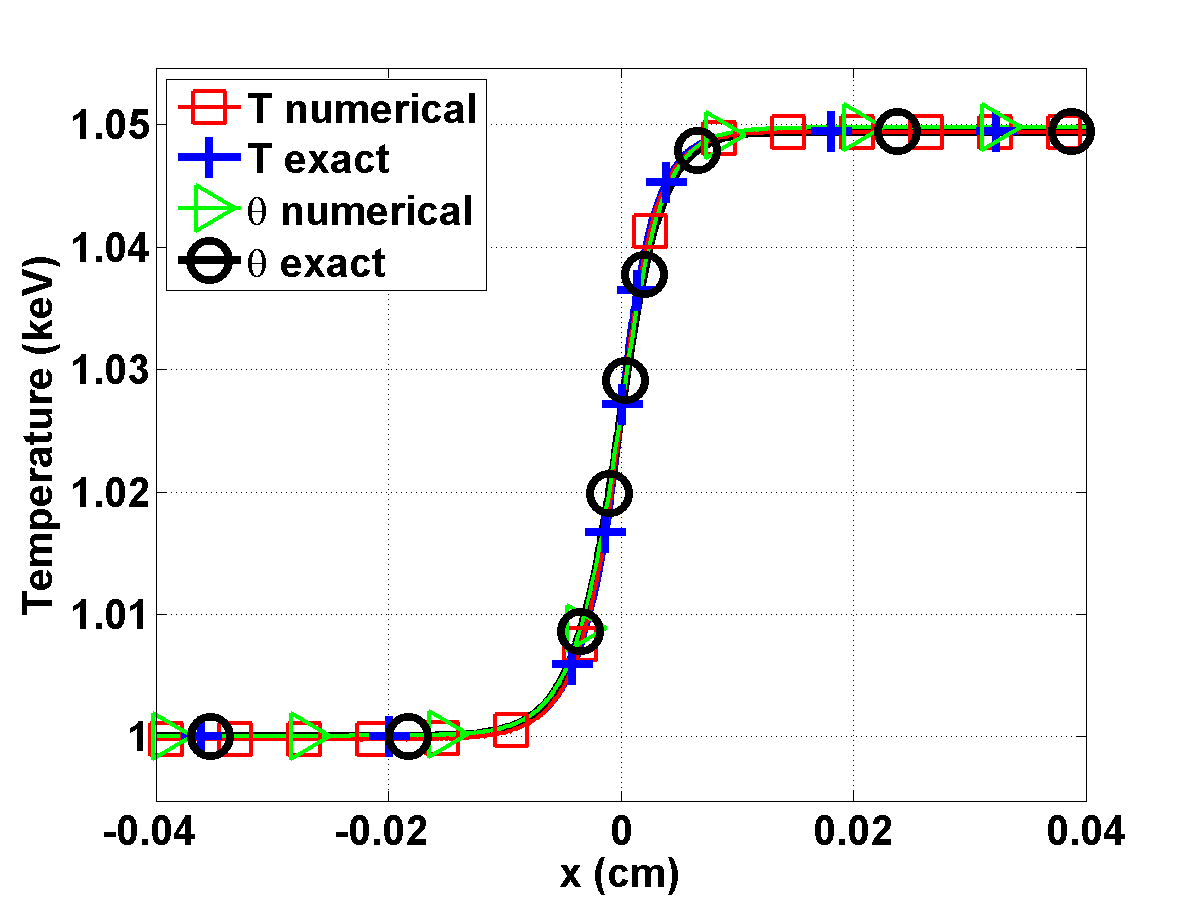
\includegraphics[width=0.4\textwidth]{figures_jcp/Mach_1p05_nel_500_temperature.png}
}
\subfigure[Material density]{
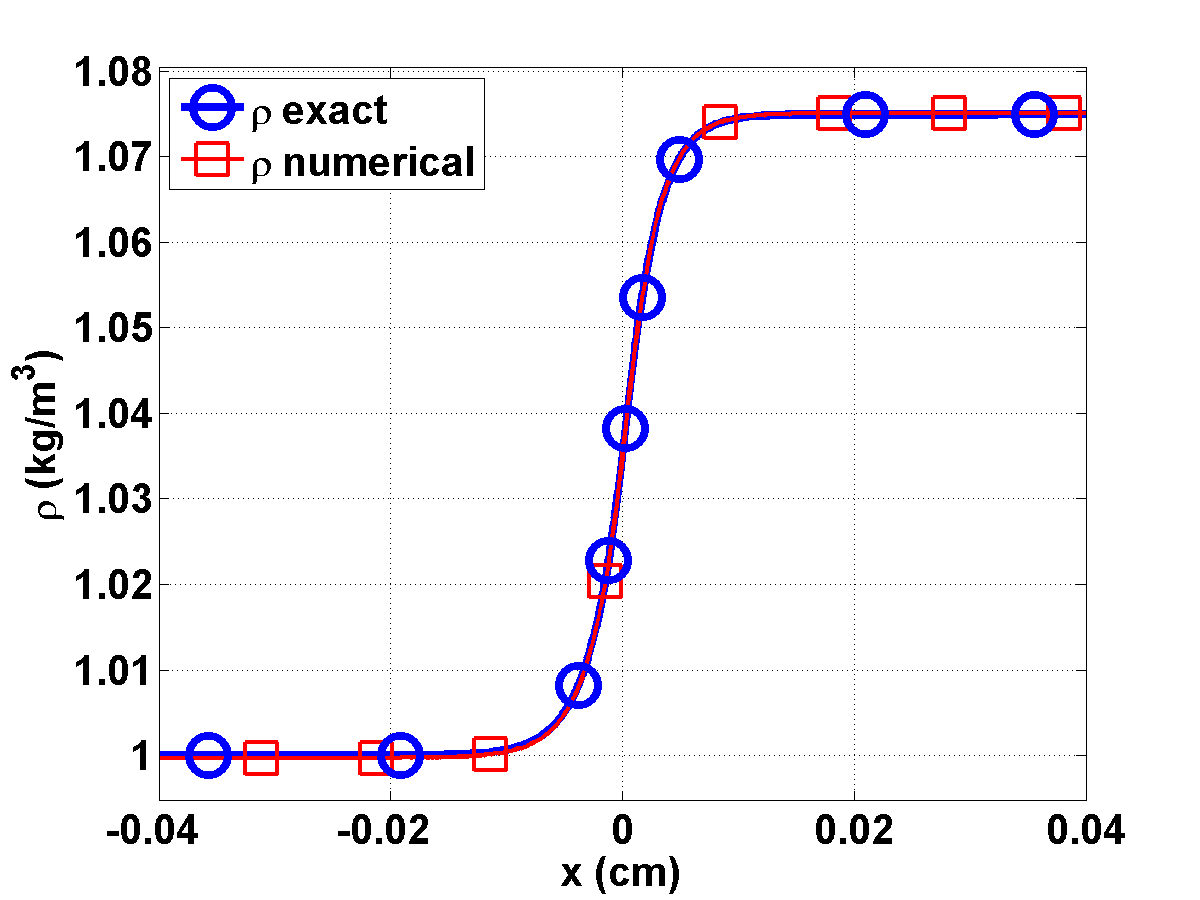
\includegraphics[width=0.4\textwidth]{figures_jcp/Mach_1p05_nel_500_density.png}
}
\\
\vspace{-3mm}
%
\subfigure[Viscosity coefficients]{
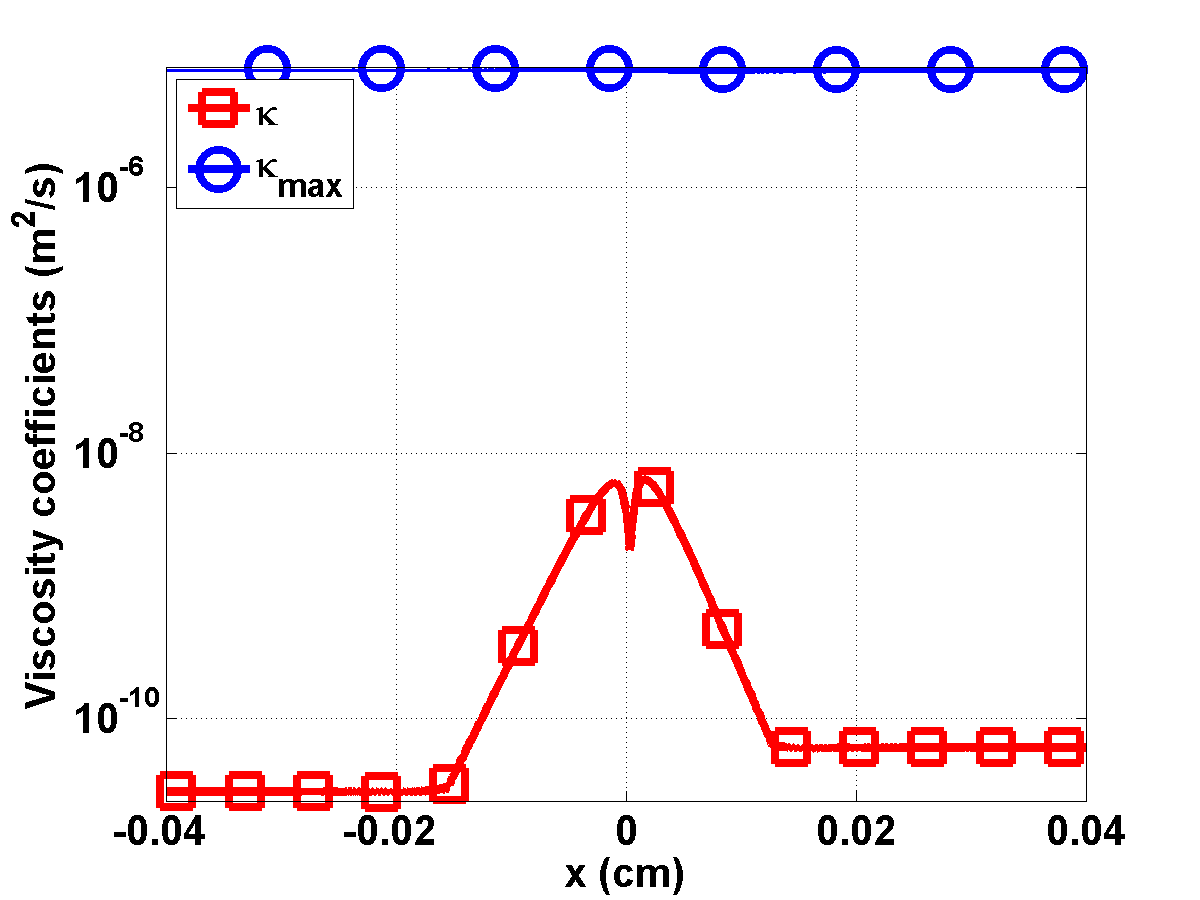
\includegraphics[width=0.4\textwidth]{figures_jcp/Mach_1p05_nel_500_viscosity.png}
}
\end{figure}

\end{frame}
%%%%%%%%%%%%%%%%%%%%%%%%%%%%%%%%%%%%%%%%%%%%%%%%%%%%%%%%%%%%%%%%%%%%


%%%%%%%%%%%%%%%%%%%%%%%%%%%%%%%%%%%%%%%%%%%%%%%%%%%%%%%%%%%%%%%%%%%%
\begin{frame}{Steady-state solution for Mach 2}
\setcounter{subfigure}{0}% Reset subfigure counter

\begin{figure}[H]
\centering
\subfigure[Temperatures]{
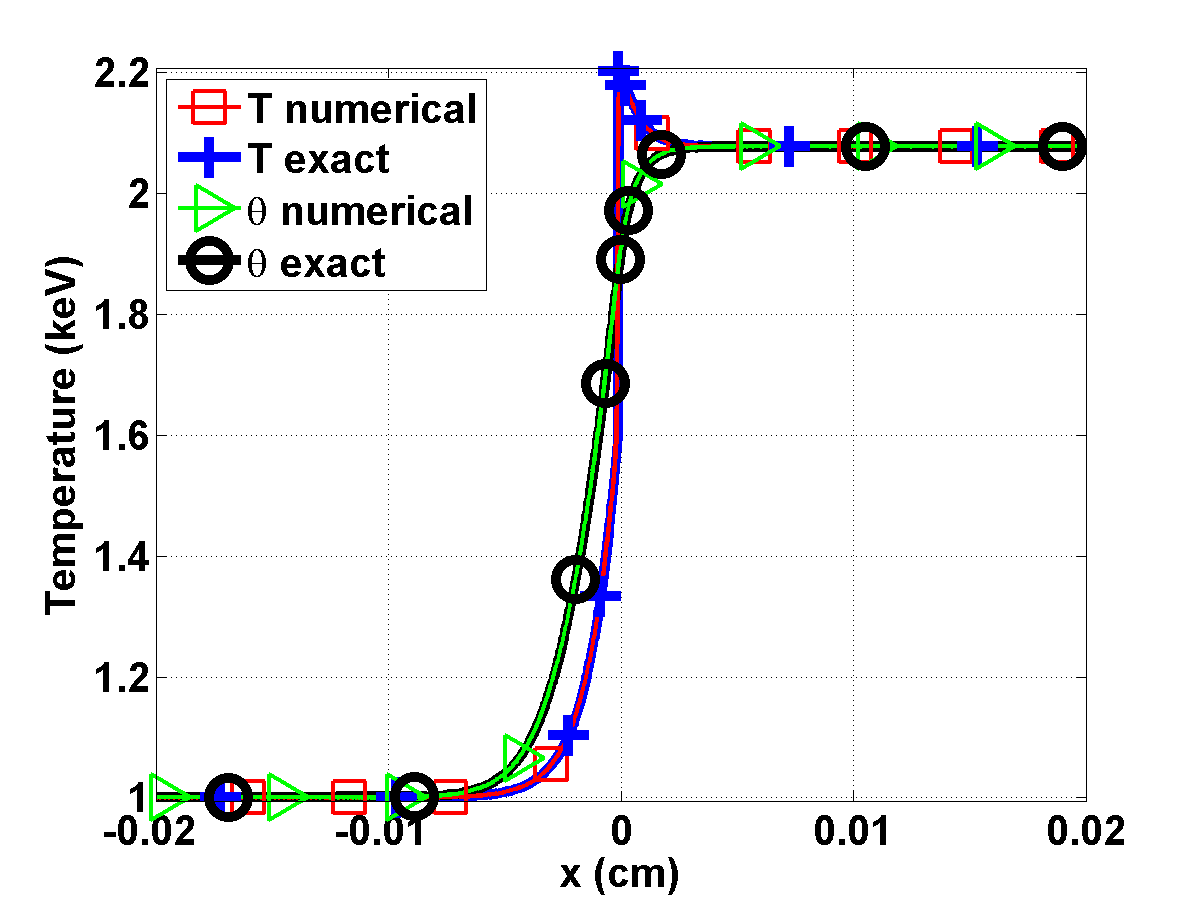
\includegraphics[width=0.4\textwidth]{figures_jcp/Mach_2_nel_2000_temperature.png}
}
\subfigure[Material density]{
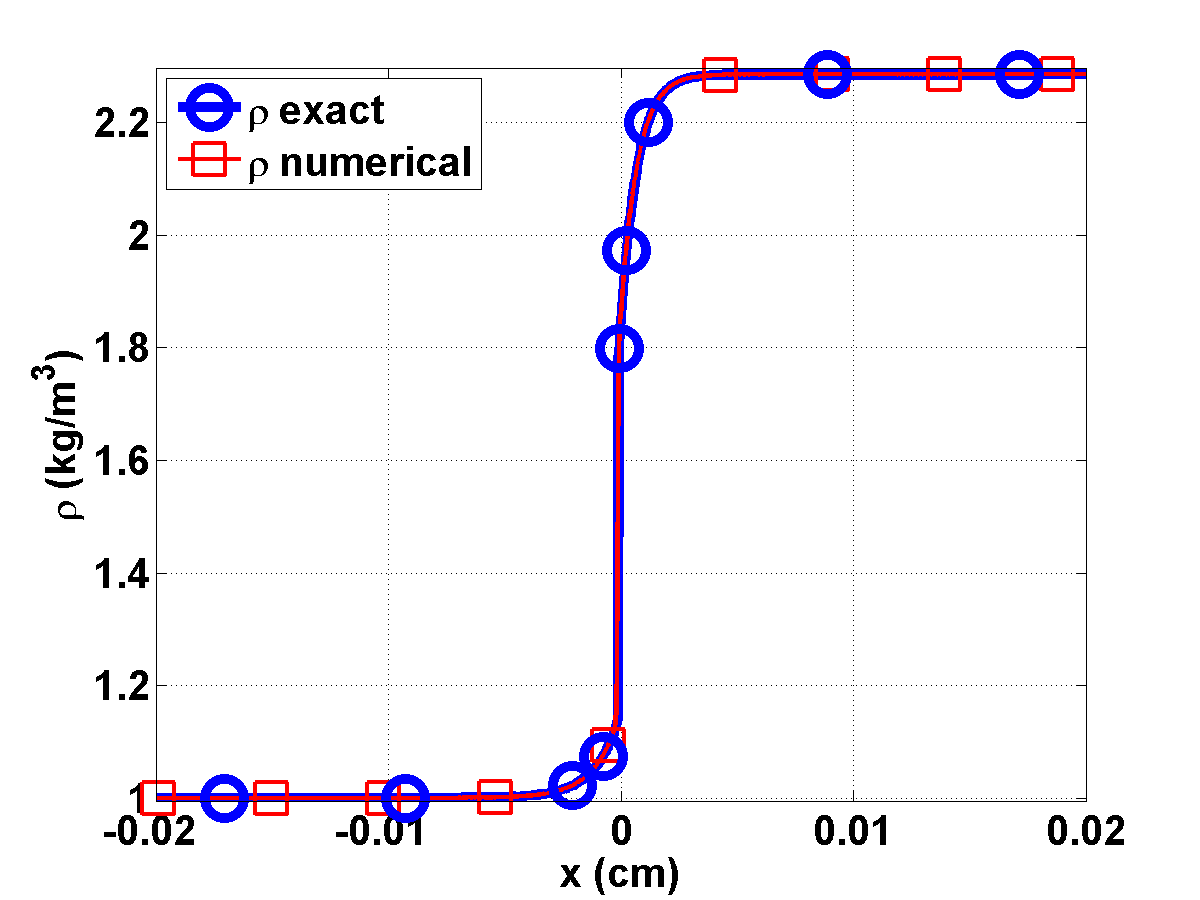
\includegraphics[width=0.4\textwidth]{figures_jcp/Mach_2_nel_2000_density.png}
}
\\
\vspace{-3mm}
%
\subfigure[Viscosity coefficients]{
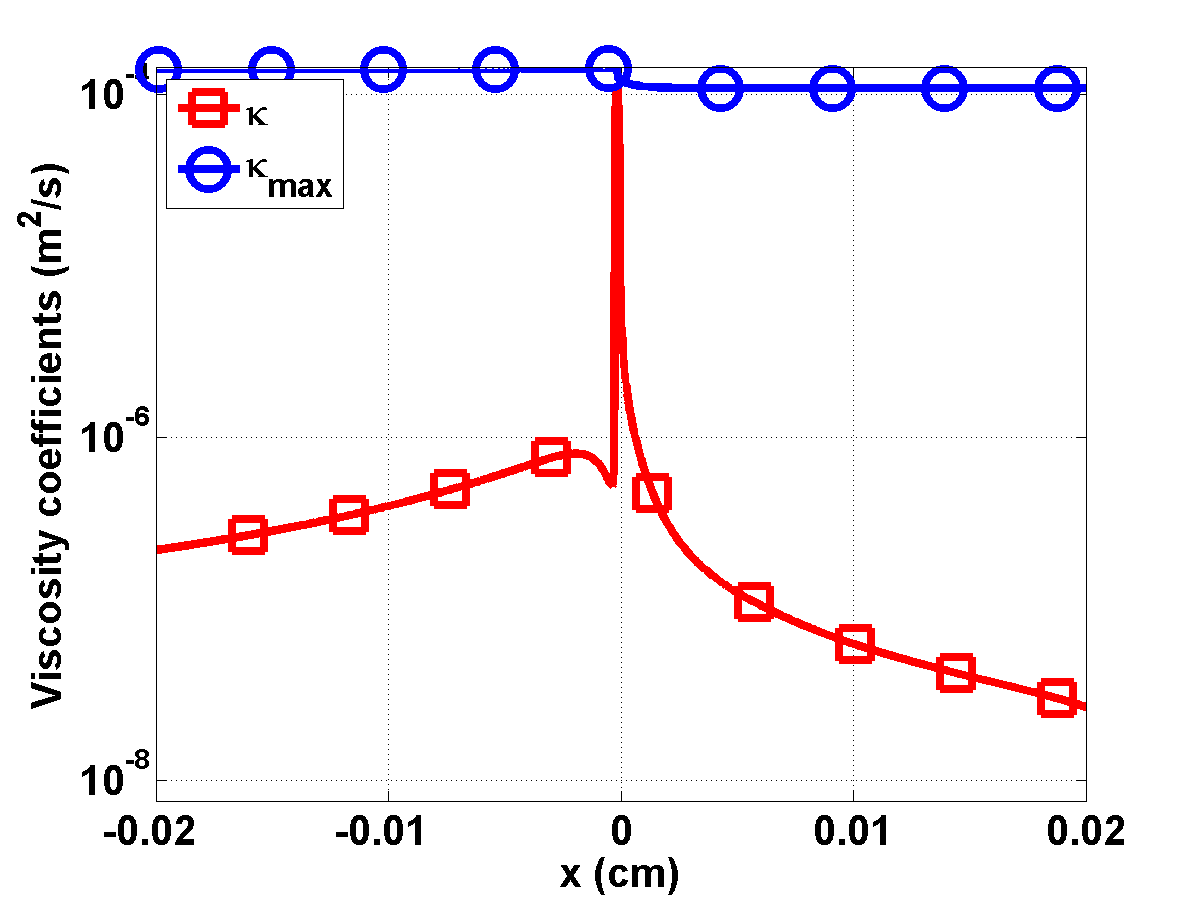
\includegraphics[width=0.4\textwidth]{figures_jcp/Mach_2_nel_2000_viscosity.png}
}
\end{figure}

\end{frame}
%%%%%%%%%%%%%%%%%%%%%%%%%%%%%%%%%%%%%%%%%%%%%%%%%%%%%%%%%%%%%%%%%%%%

%%%%%%%%%%%%%%%%%%%%%%%%%%%%%%%%%%%%%%%%%%%%%%%%%%%%%%%%%%%%%%%%%%%%
\begin{frame}{Steady-state solution for Mach 5}
\setcounter{subfigure}{0}% Reset subfigure counter

\begin{figure}[H]
\centering
\subfigure[Temperatures]{
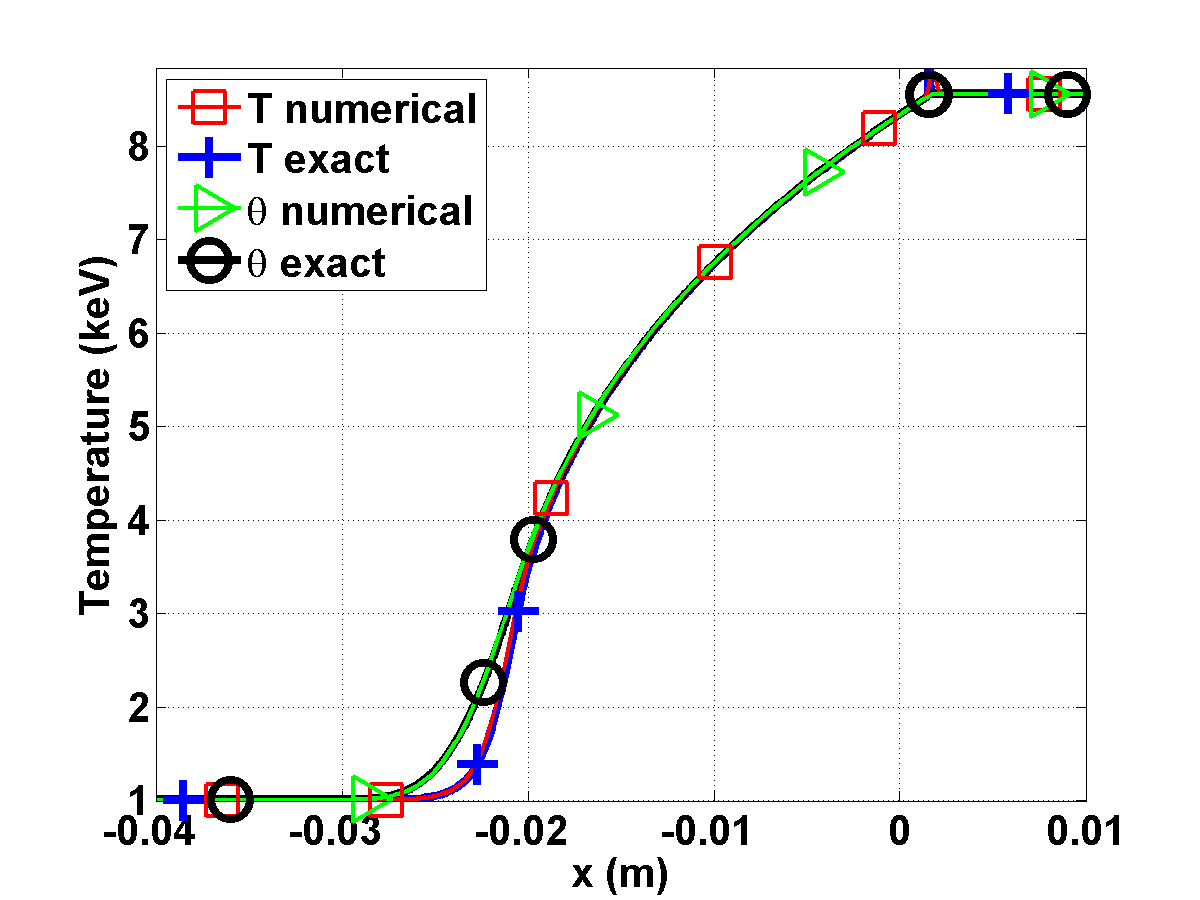
\includegraphics[width=0.4\textwidth]{figures_jcp/Mach_5_nel_1000_temperature.png}
}
\subfigure[Material density]{
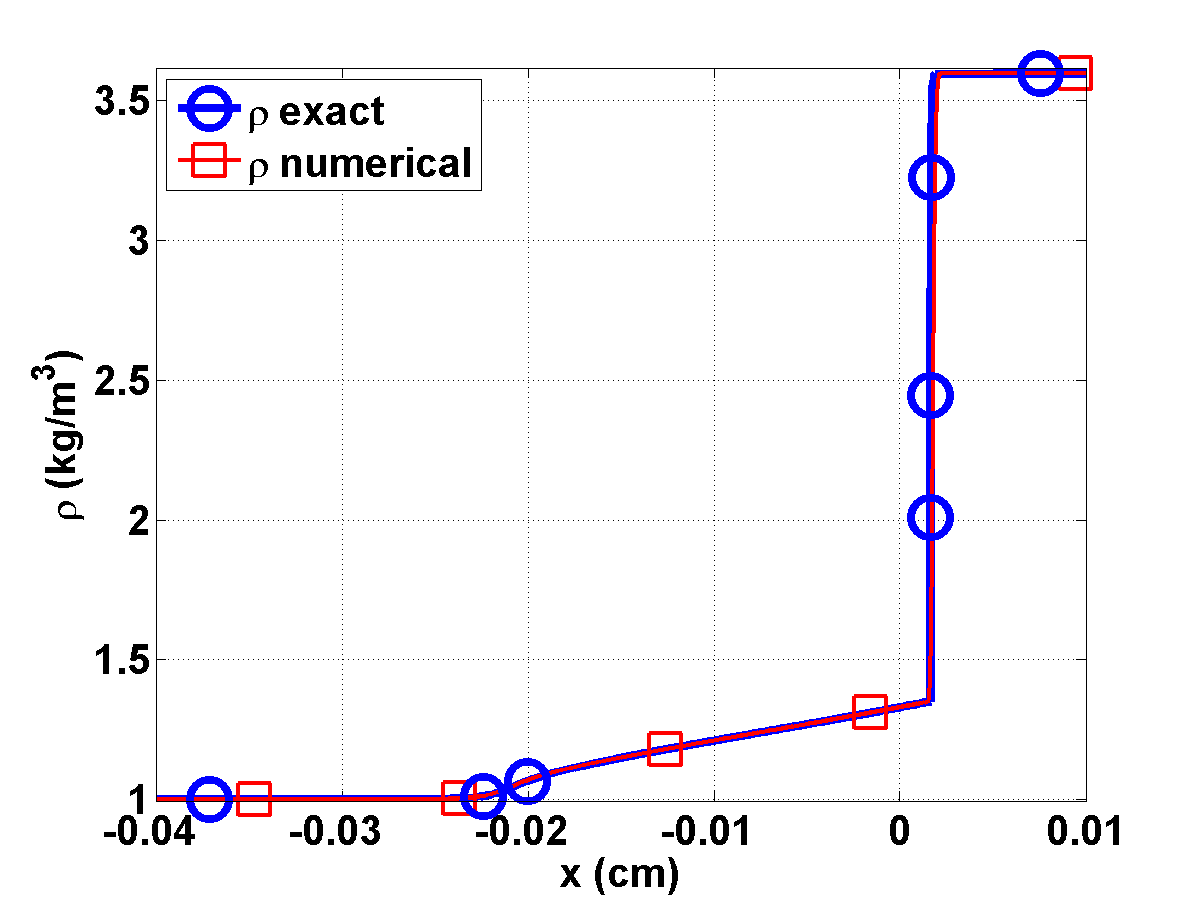
\includegraphics[width=0.4\textwidth]{figures_jcp/Mach_5_nel_2000_density.png}
}
\\
\vspace{-3mm}
%
\subfigure[Viscosity coefficients]{
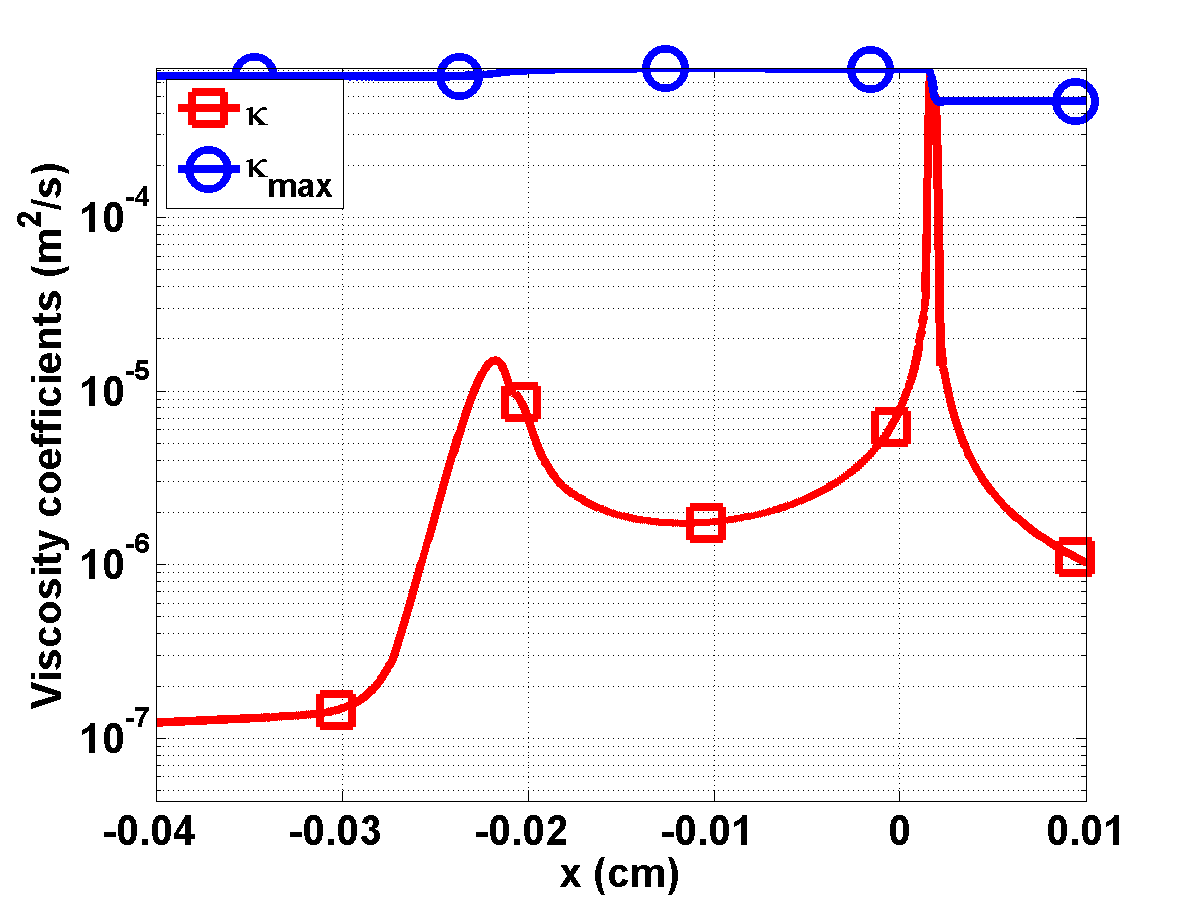
\includegraphics[width=0.4\textwidth]{figures_jcp/Mach_5_nel_2000_viscosity.png}
}
\subfigure[Zoom at the Z spike]{
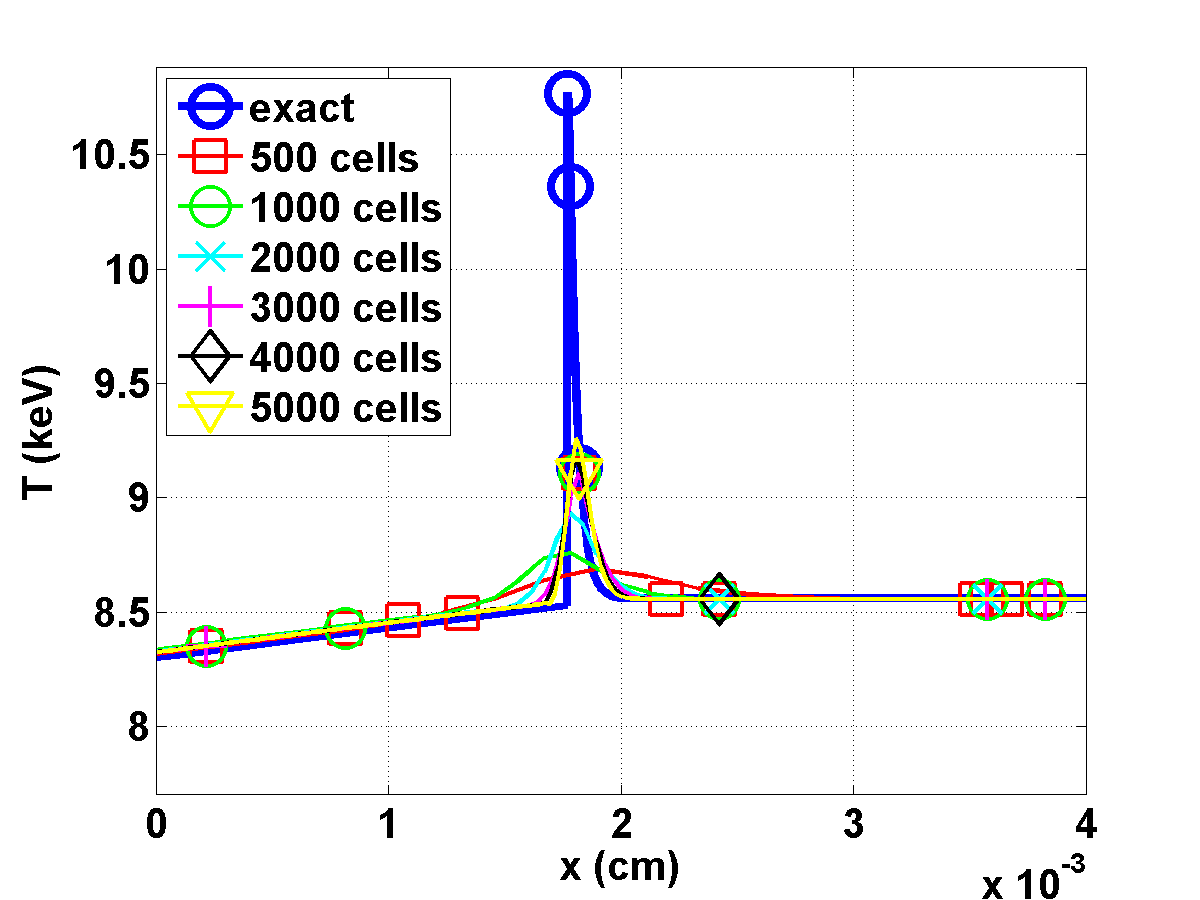
\includegraphics[width=0.4\textwidth]{figures_jcp/Mach_5_comparison.png}
}
\end{figure}


\end{frame}
%%%%%%%%%%%%%%%%%%%%%%%%%%%%%%%%%%%%%%%%%%%%%%%%%%%%%%%%%%%%%%%%%%%%

%%%%%%%%%%%%%%%%%%%%%%%%%%%%%%%%%%%%%%%%%%%%%%%%%%%%%%%%%%%%%%%%%%%%
\begin{frame}{Steady-state solution for Mach 50}
\setcounter{subfigure}{0}% Reset subfigure counter

\begin{figure}[H]
\centering
\subfigure[Temperatures]{
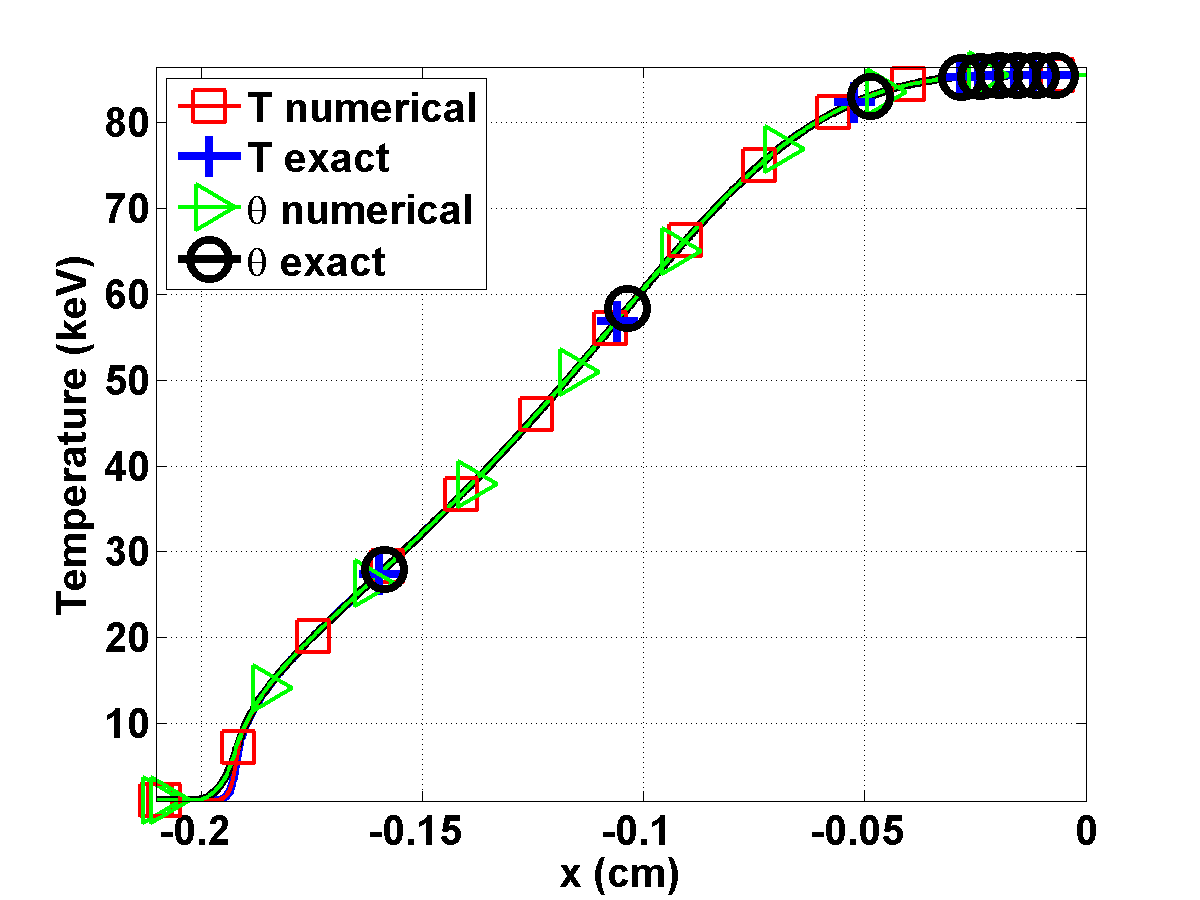
\includegraphics[width=0.4\textwidth]{figures_jcp/Mach_50_nel_1000_temperature.png}
}
\subfigure[Material density]{
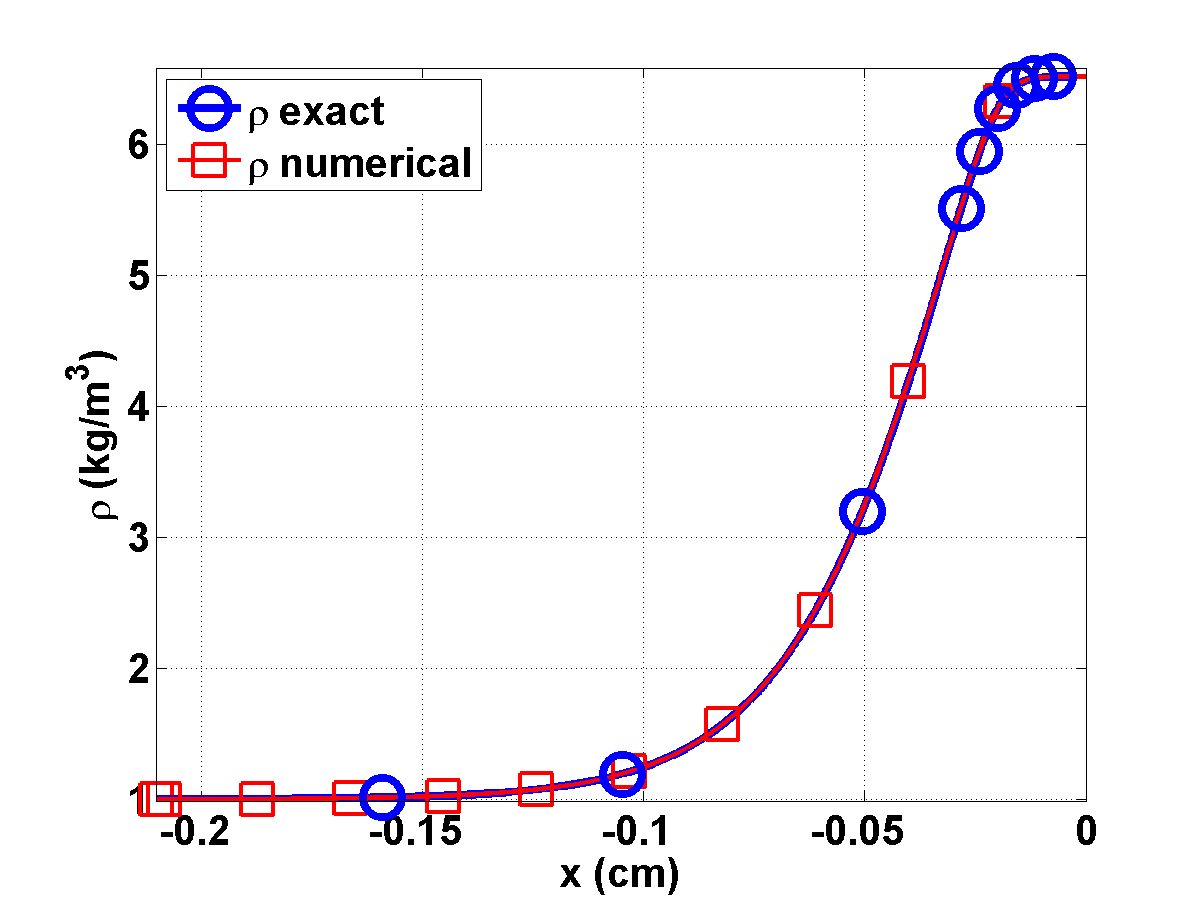
\includegraphics[width=0.4\textwidth]{figures_jcp/Mach_50_nel_1000_density.png}
}
\\
\vspace{-3mm}
%
\subfigure[Viscosity coefficients]{
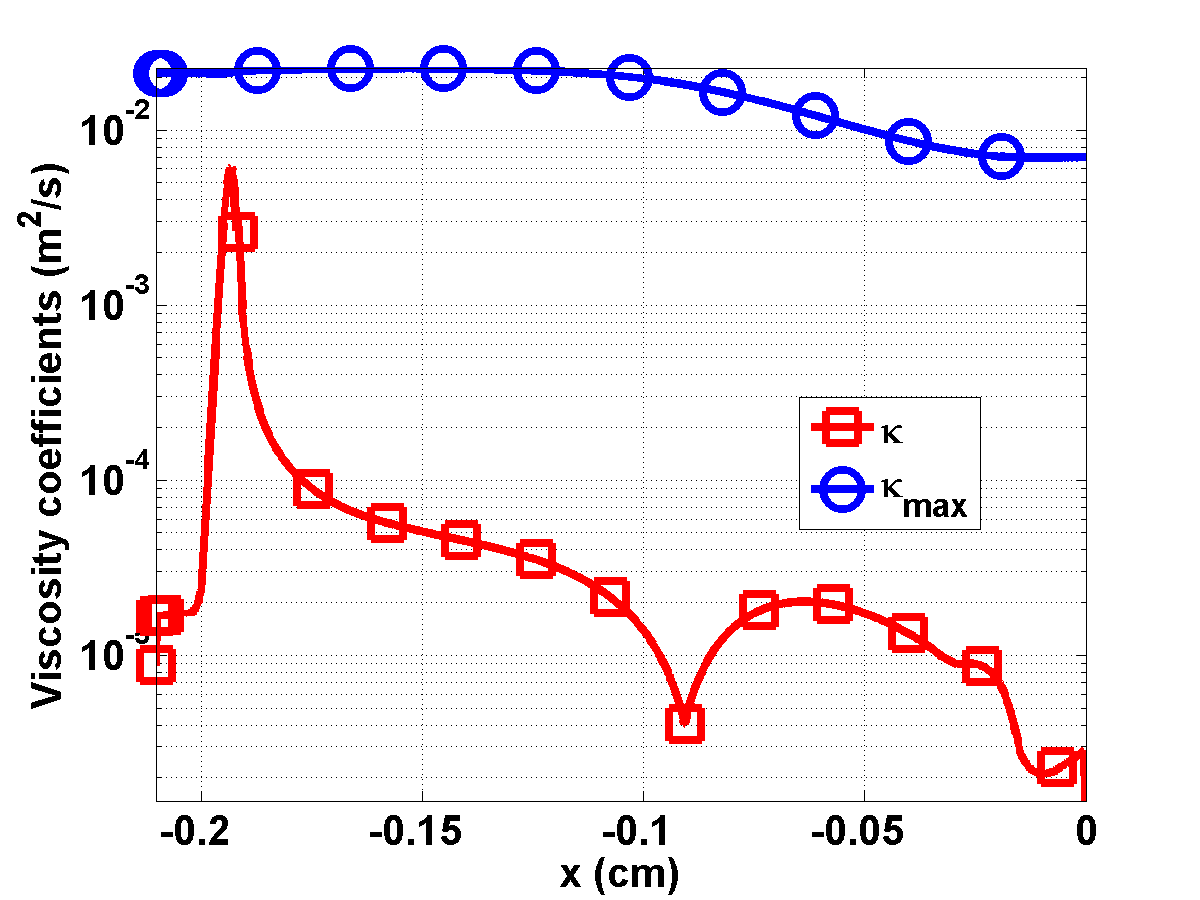
\includegraphics[width=0.4\textwidth]{figures_jcp/Mach_50_nel_1000_viscosity.png}
}
\end{figure}

\end{frame}
%%%%%%%%%%%%%%%%%%%%%%%%%%%%%%%%%%%%%%%%%%%%%%%%%%%%%%%%%%%%%%%%%%%%


%%%%%%%%%%%%%%%%%%%%%%%%%%%%%%%%%%%%%%%%%%%%%%%%%%%%%%%%%%%%%%%%%%%%
\subsection{Temperature-dependent opacities}
%%%%%%%%%%%%%%%%%%%%%%%%%%%%%%%%%%%%%%%%%%%%%%%%%%%%%%%%%%%%%%%%%%%%

%%%%%%%%%%%%%%%%%%%%%%%%%%%%%%%%%%%%%%%%%%%%%%%%%%%%%%%%%%%%%%%%%%%%
\begin{frame}{Steady-state solution for Mach 3:  \tcr{density}, 500 cells}

Now, results with temperature-dependent opacities:
\begin{figure}[H]
\centering
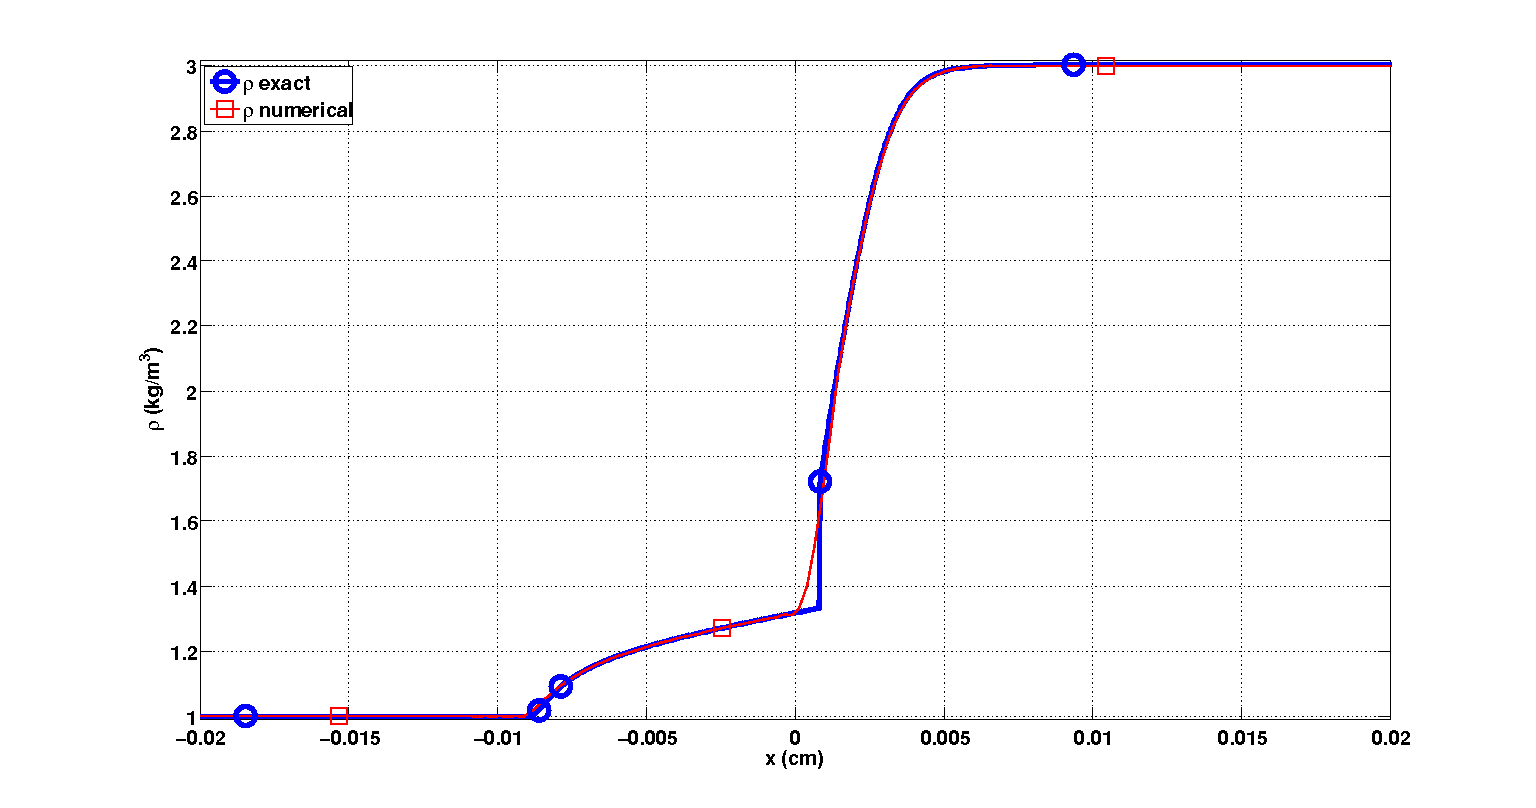
\includegraphics[width=0.99\textwidth]{figures_new_results/mach-3-temp-dpt-xs-density-500.png}
\end{figure}

\end{frame}
%%%%%%%%%%%%%%%%%%%%%%%%%%%%%%%%%%%%%%%%%%%%%%%%%%%%%%%%%%%%%%%%%%%%

%%%%%%%%%%%%%%%%%%%%%%%%%%%%%%%%%%%%%%%%%%%%%%%%%%%%%%%%%%%%%%%%%%%%
\begin{frame}{Steady-state solution for Mach 3:  \tcr{density}, 1000 cells}

\begin{figure}[H]
\centering
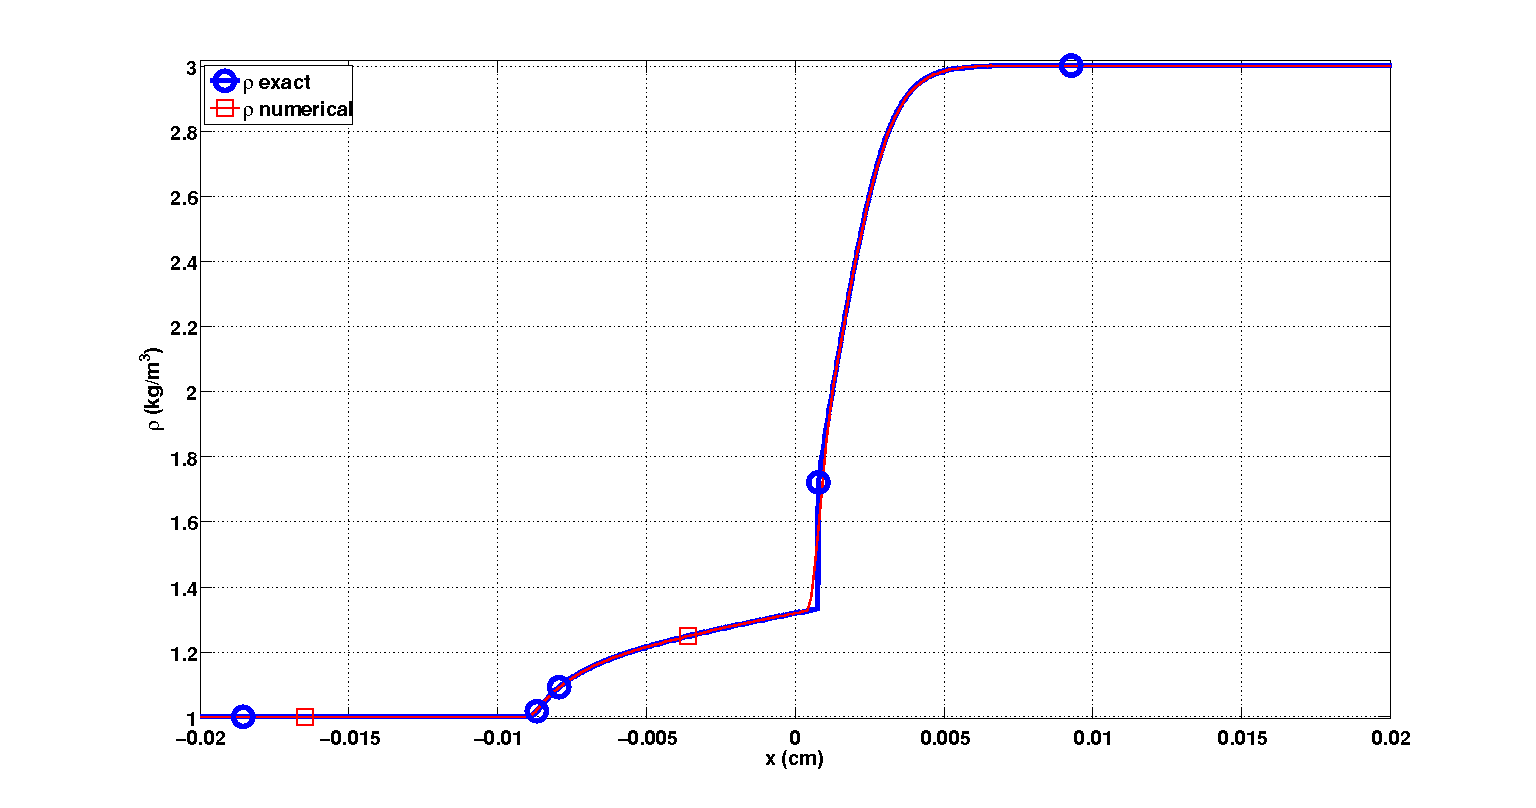
\includegraphics[width=0.99\textwidth]{figures_new_results/mach-3-temp-dpt-xs-density-1000.png}
\end{figure}

\end{frame}
%%%%%%%%%%%%%%%%%%%%%%%%%%%%%%%%%%%%%%%%%%%%%%%%%%%%%%%%%%%%%%%%%%%%

%%%%%%%%%%%%%%%%%%%%%%%%%%%%%%%%%%%%%%%%%%%%%%%%%%%%%%%%%%%%%%%%%%%%
\begin{frame}{Steady-state solution for Mach 3:  \tcr{density}, 2000 cells}

\begin{figure}[H]
\centering
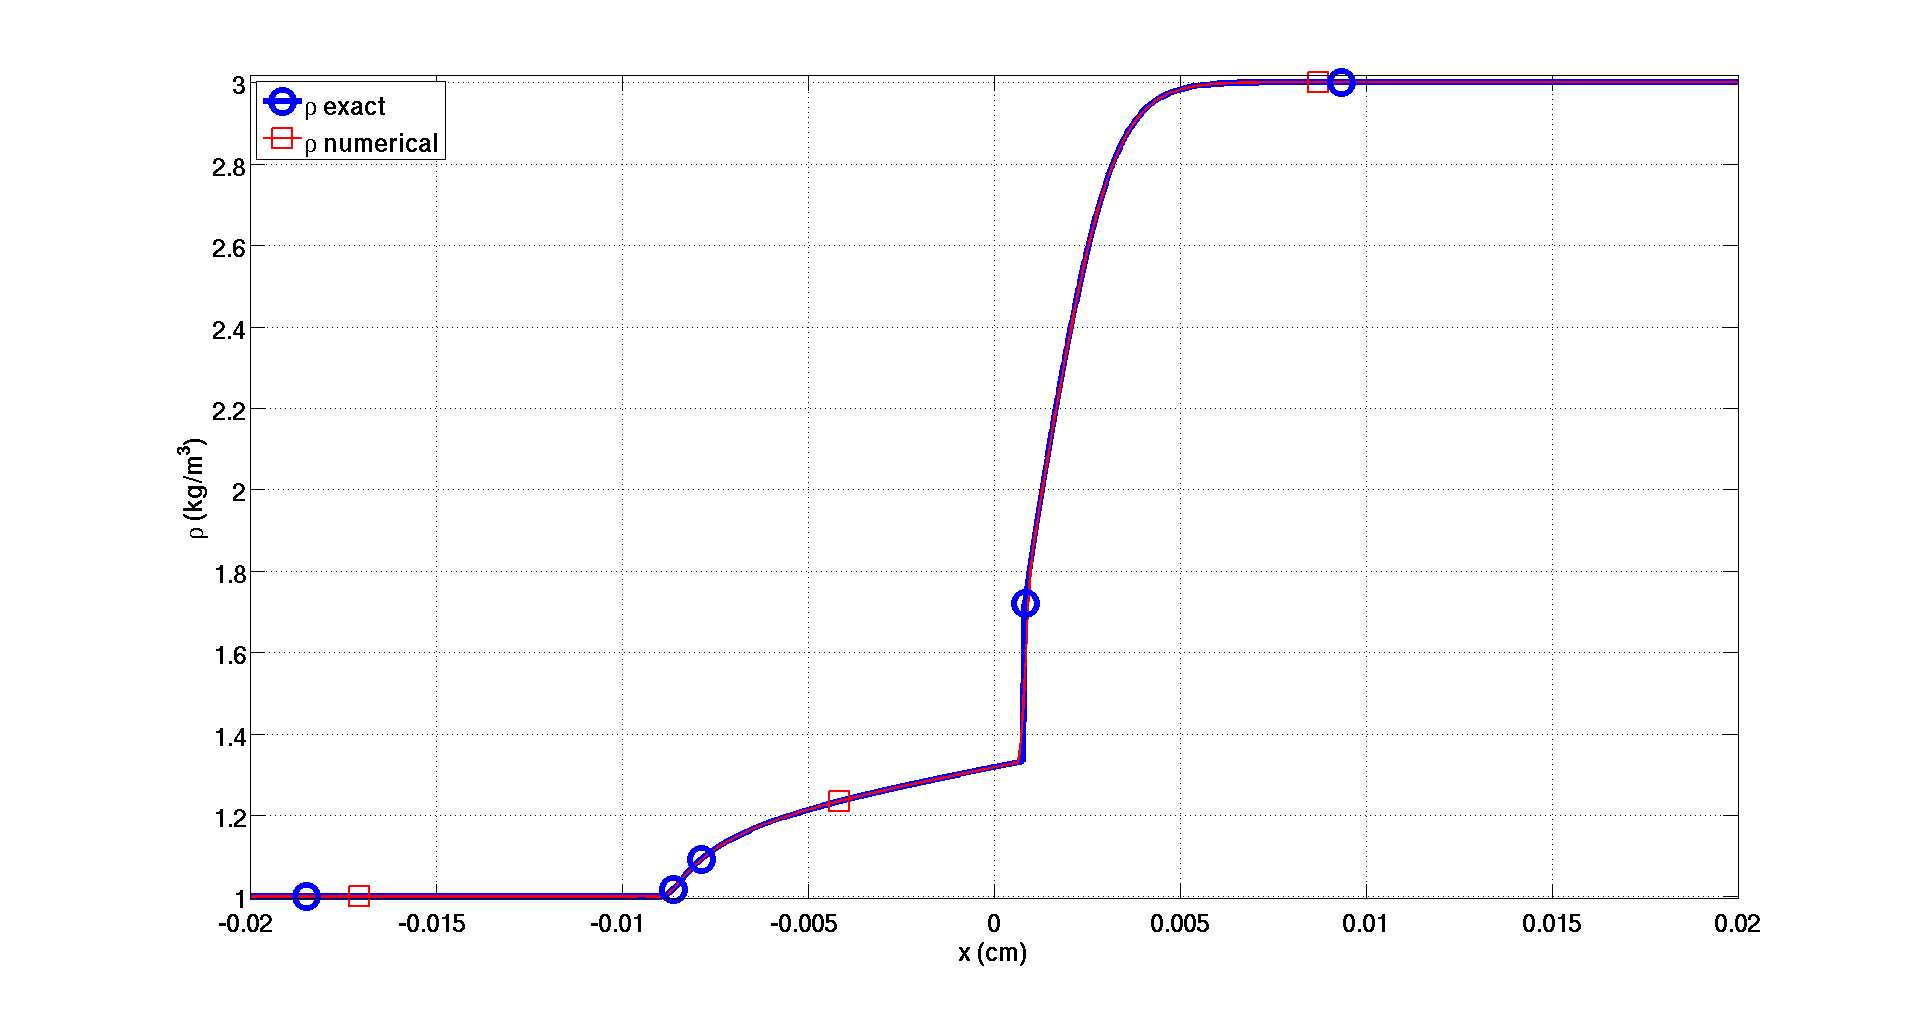
\includegraphics[width=0.99\textwidth]{figures_new_results/mach-3-temp-dpt-xs-density-2000.png}
\end{figure}

\end{frame}
%%%%%%%%%%%%%%%%%%%%%%%%%%%%%%%%%%%%%%%%%%%%%%%%%%%%%%%%%%%%%%%%%%%%

%%%%%%%%%%%%%%%%%%%%%%%%%%%%%%%%%%%%%%%%%%%%%%%%%%%%%%%%%%%%%%%%%%%%
\begin{frame}{Steady-state solution for Mach 3:  \tcr{temperature}, 500 cells}

\begin{figure}[H]
\centering
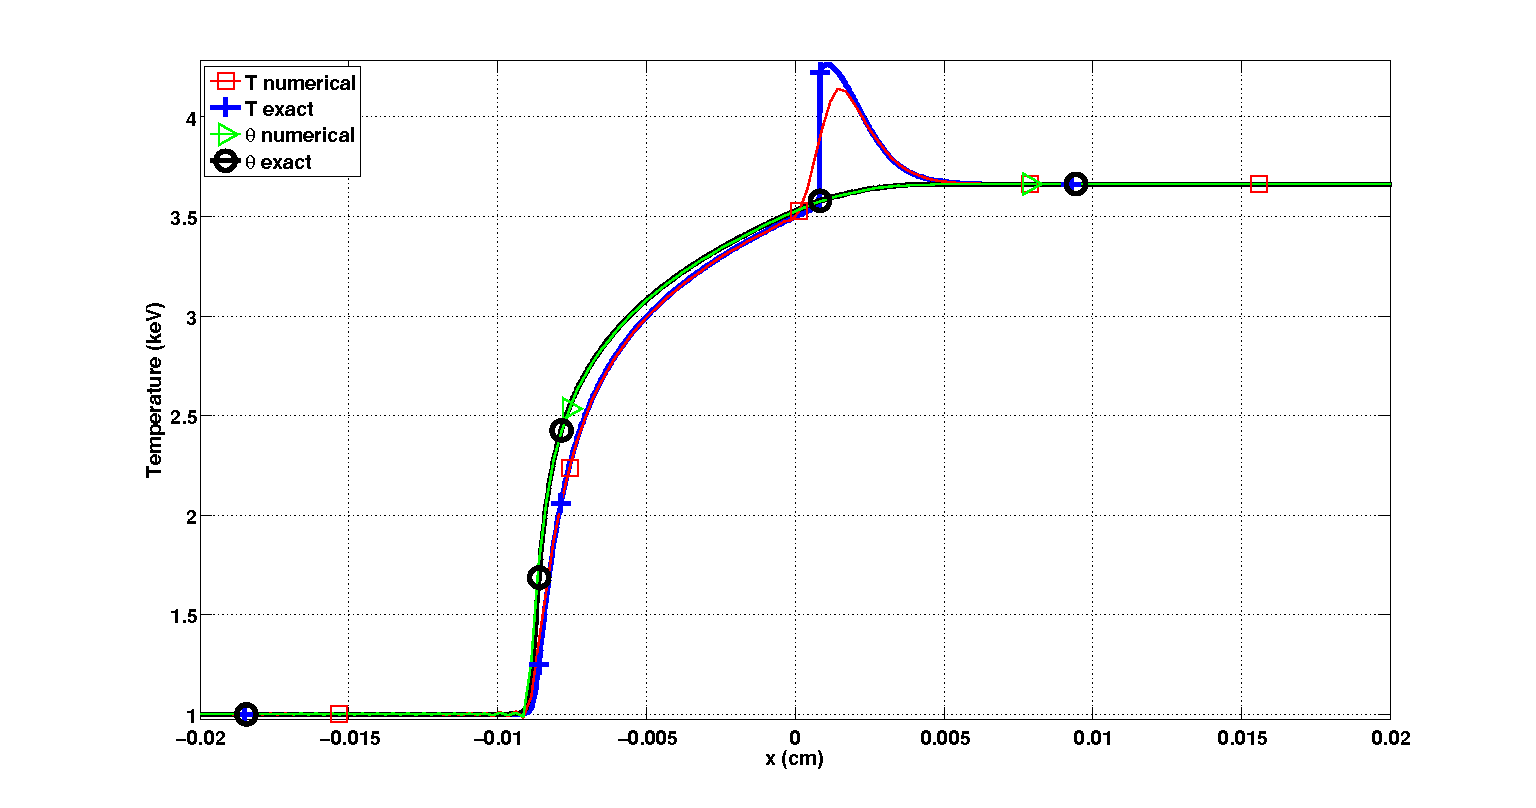
\includegraphics[width=0.99\textwidth]{figures_new_results/mach-3-temp-dpt-xs-temperature-500.png}
\end{figure}

\end{frame}
%%%%%%%%%%%%%%%%%%%%%%%%%%%%%%%%%%%%%%%%%%%%%%%%%%%%%%%%%%%%%%%%%%%%

%%%%%%%%%%%%%%%%%%%%%%%%%%%%%%%%%%%%%%%%%%%%%%%%%%%%%%%%%%%%%%%%%%%%
\begin{frame}{Steady-state solution for Mach 3:  \tcr{temperature}, 1000 cells}

\begin{figure}[H]
\centering
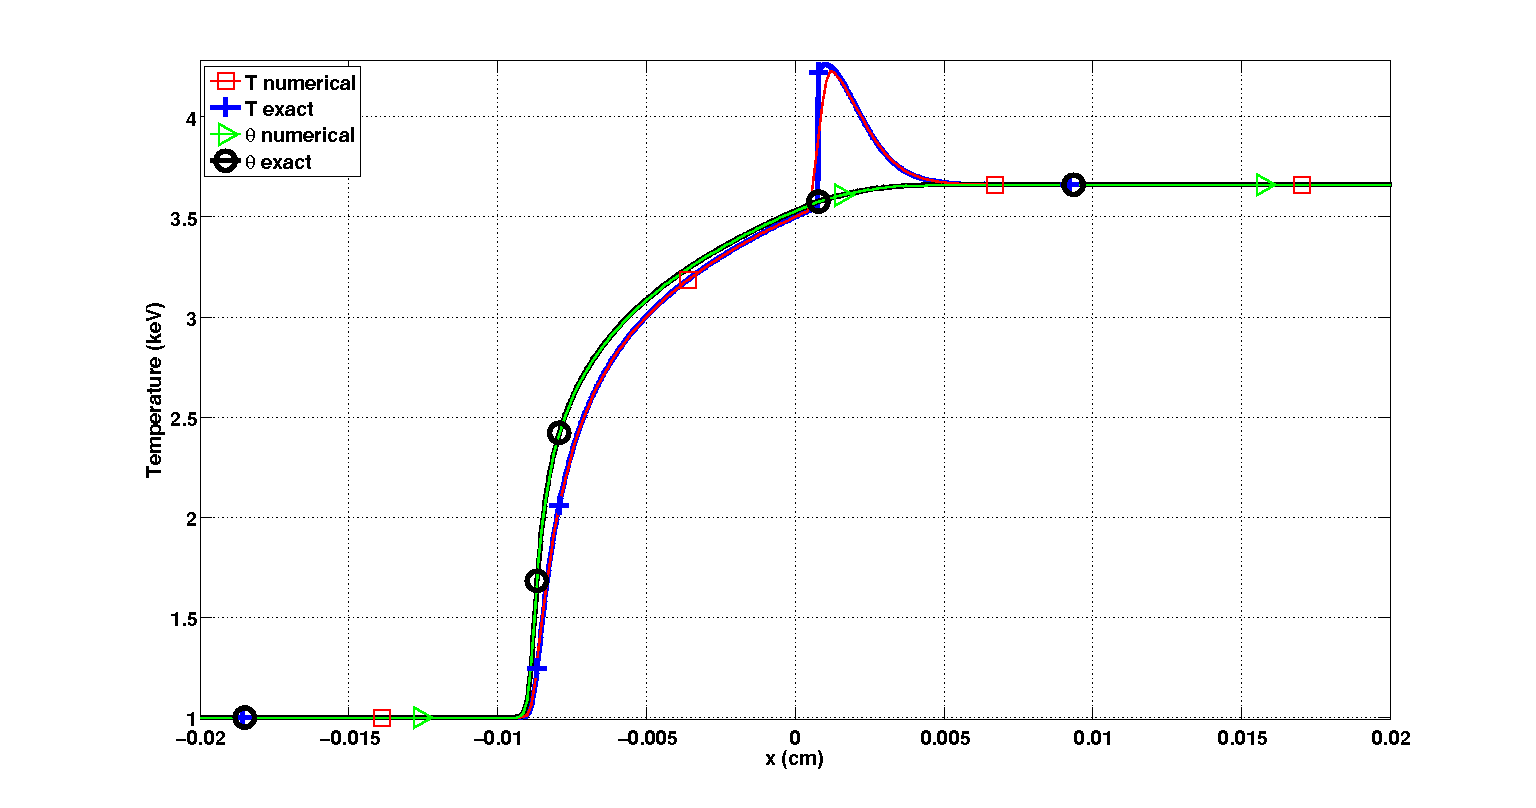
\includegraphics[width=0.99\textwidth]{figures_new_results/mach-3-temp-dpt-xs-temperature-1000.png}
\end{figure}

\end{frame}
%%%%%%%%%%%%%%%%%%%%%%%%%%%%%%%%%%%%%%%%%%%%%%%%%%%%%%%%%%%%%%%%%%%%

%%%%%%%%%%%%%%%%%%%%%%%%%%%%%%%%%%%%%%%%%%%%%%%%%%%%%%%%%%%%%%%%%%%%
\begin{frame}{Steady-state solution for Mach 3:  \tcr{temperature}, 2000 cells}

\begin{figure}[H]
\centering
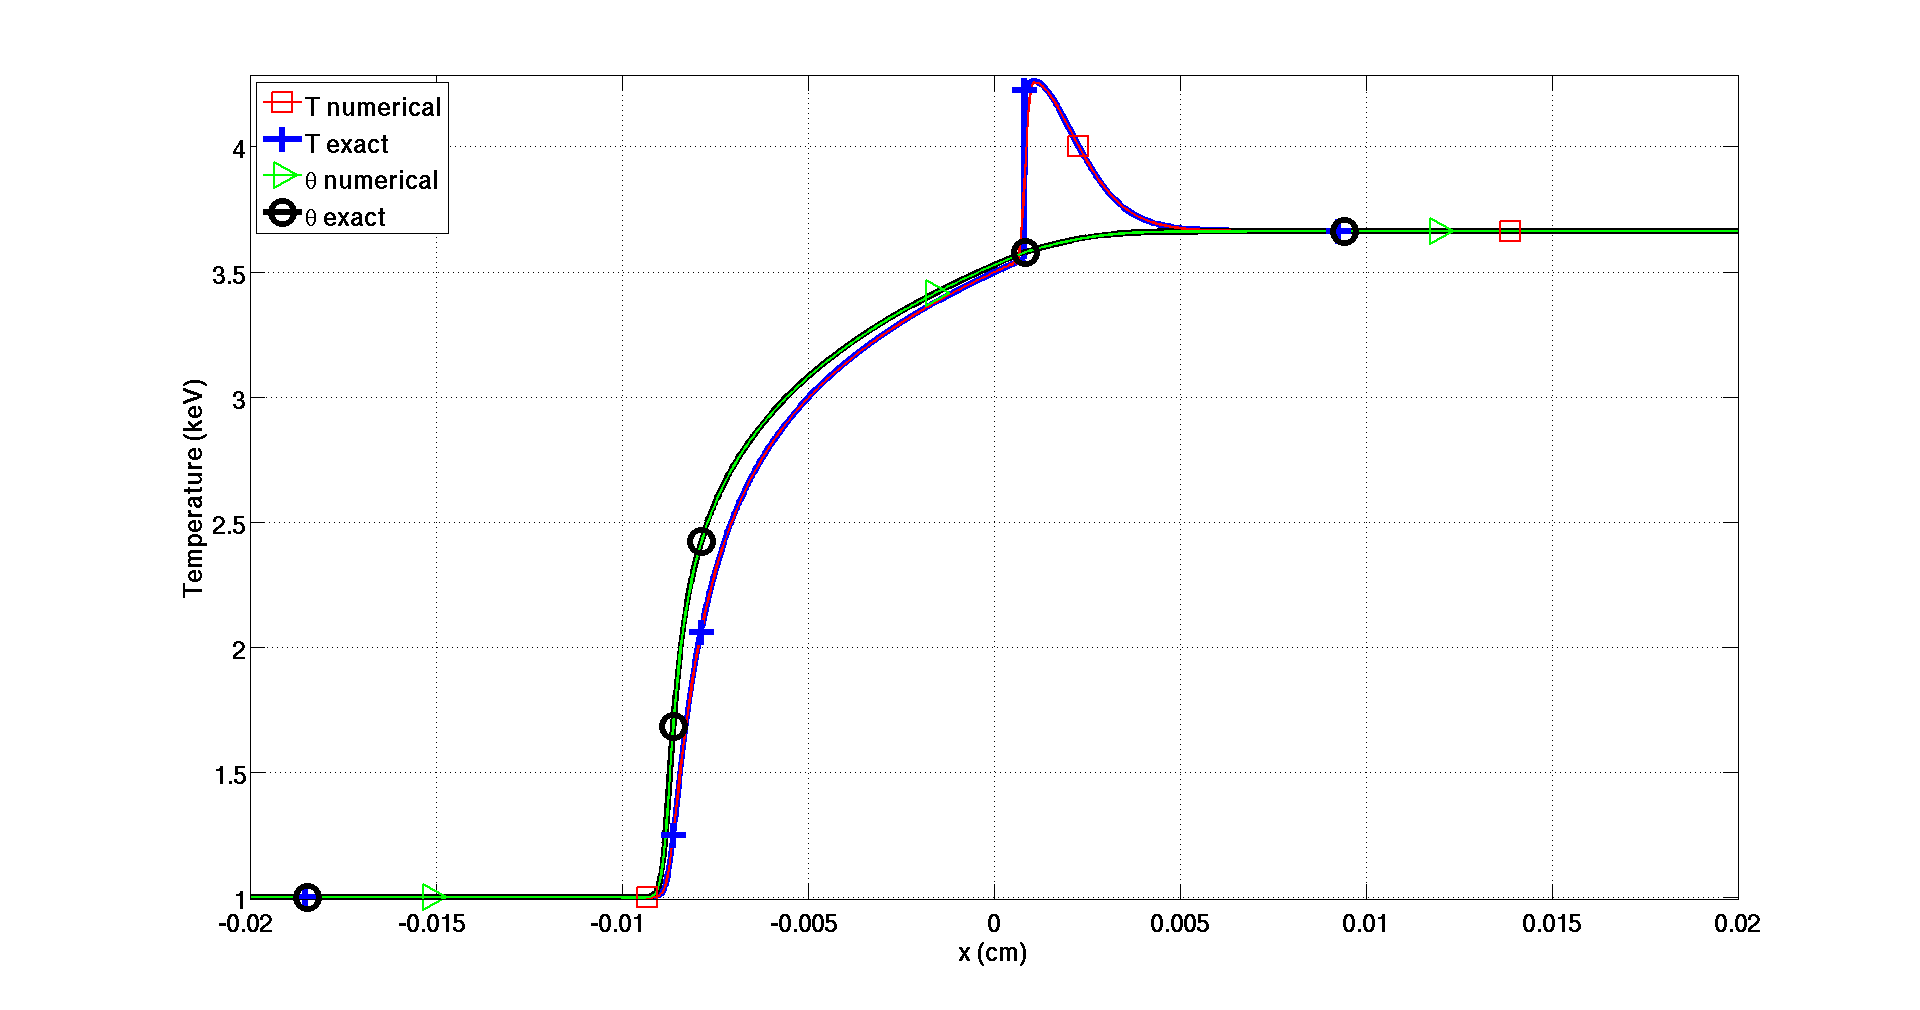
\includegraphics[width=0.99\textwidth]{figures_new_results/mach-3-temp-dpt-xs-temperature-2000.png}
\end{figure}

\end{frame}
%%%%%%%%%%%%%%%%%%%%%%%%%%%%%%%%%%%%%%%%%%%%%%%%%%%%%%%%%%%%%%%%%%%%

%%%%%%%%%%%%%%%%%%%%%%%%%%%%%%%%%%%%%%%%%%%%%%%%%%%%%%%%%%%%%%%%%%%%
\begin{frame}{Steady-state solution for Mach 3:  \tcr{viscosity}, 500 cells}

\begin{figure}[H]
\centering
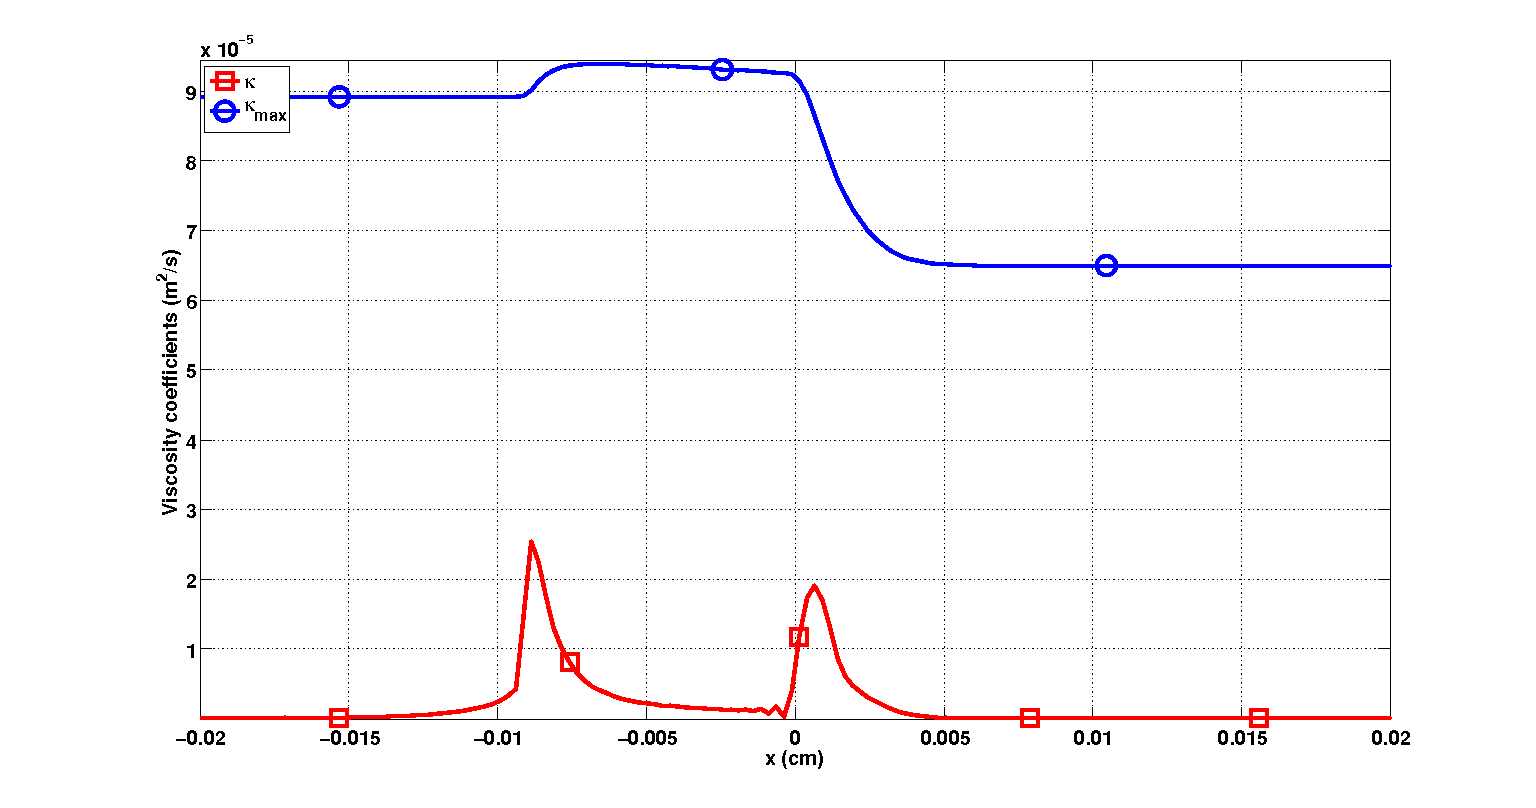
\includegraphics[width=0.99\textwidth]{figures_new_results/mach-3-temp-dpt-xs-viscosity-500.png}
\end{figure}

\end{frame}
%%%%%%%%%%%%%%%%%%%%%%%%%%%%%%%%%%%%%%%%%%%%%%%%%%%%%%%%%%%%%%%%%%%%

%%%%%%%%%%%%%%%%%%%%%%%%%%%%%%%%%%%%%%%%%%%%%%%%%%%%%%%%%%%%%%%%%%%%
\begin{frame}{Steady-state solution for Mach 3:  \tcr{viscosity}, 1000 cells}

\begin{figure}[H]
\centering
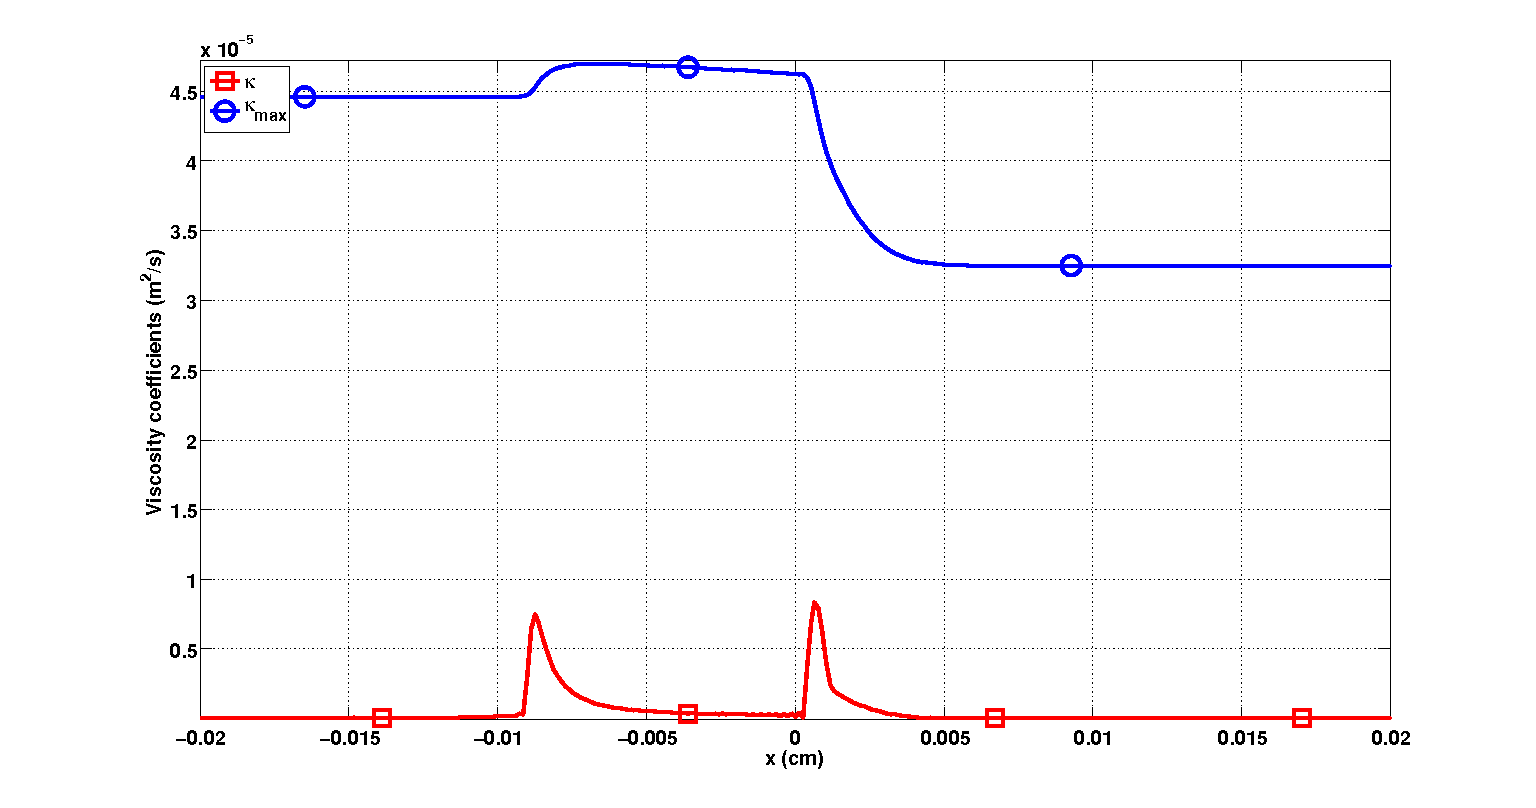
\includegraphics[width=0.99\textwidth]{figures_new_results/mach-3-temp-dpt-xs-viscosity-1000.png}
\end{figure}

\end{frame}
%%%%%%%%%%%%%%%%%%%%%%%%%%%%%%%%%%%%%%%%%%%%%%%%%%%%%%%%%%%%%%%%%%%%

%%%%%%%%%%%%%%%%%%%%%%%%%%%%%%%%%%%%%%%%%%%%%%%%%%%%%%%%%%%%%%%%%%%%
\begin{frame}{Steady-state solution for Mach 3:  \tcr{viscosity}, 2000 cells}

\begin{figure}[H]
\centering
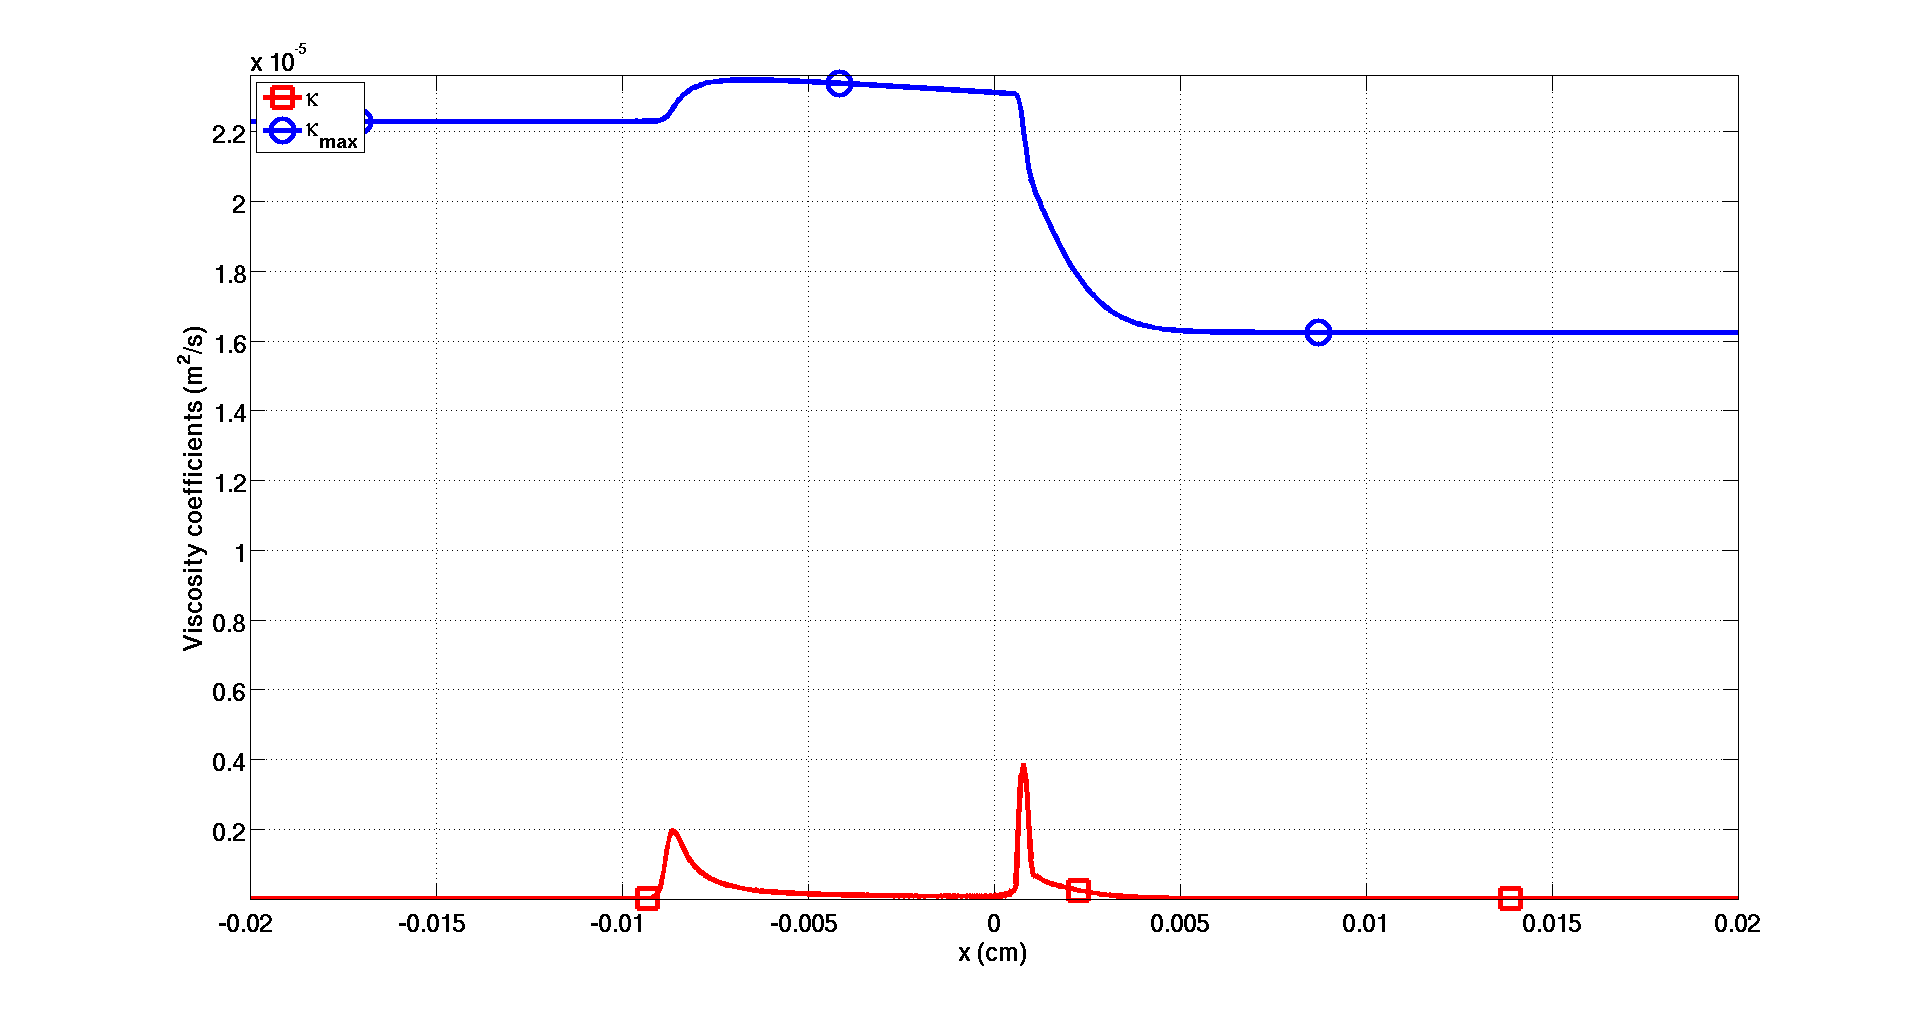
\includegraphics[width=0.99\textwidth]{figures_new_results/mach-3-temp-dpt-xs-viscosity-2000.png}
\end{figure}

\end{frame}
%%%%%%%%%%%%%%%%%%%%%%%%%%%%%%%%%%%%%%%%%%%%%%%%%%%%%%%%%%%%%%%%%%%%

%%%%%%%%%%%%%%%%%%%%%%%%%%%%%%%%%%%%%%%%%%%%%%%%%%%%%%%%%%%%%%%%%%%%
%%%%%%%%%%%%%%%%%%%%%%%%%%%%%%%%%%%%%%%%%%%%%%%%%%%%%%%%%%%%%%%%%%%%
\section{Conclusions}
%%%%%%%%%%%%%%%%%%%%%%%%%%%%%%%%%%%%%%%%%%%%%%%%%%%%%%%%%%%%%%%%%%%%
%%%%%%%%%%%%%%%%%%%%%%%%%%%%%%%%%%%%%%%%%%%%%%%%%%%%%%%%%%%%%%%%%%%%

%%%%%%%%%%%%%%%%%%%%%%%%%%%%%%%%%%%%%%%%%%%%%%%%%%%%%%%%%%%%%%%%%%%%
\begin{frame}

\begin{block}{Conclusions}
\begin{itemize}
\item Extended the entropy-viscosity method to the \hili{full} Grey Radiation-Hydrodynamic equations.
\item Verified the entropy minimum principle for the regularized equations GRHD.
\item Viscous regularization scales appropriately in the equilibrium-diffusion limit.
\item Numerical results are in excellent agreement with semi-analytical solutions.
\end{itemize}
\end{block}

\begin{block}{Outlook}
\begin{itemize}
\item Multi-D.
\item Replace radiation diffusion with $S_n$ radiation transport.
\item Switch solution technique to IMEX (implicit for radiation, explicit for hydro).
\item Other spatial discretization (DGFEM).
\item FCT \\
      $\to$ poster tomorrow on FCT for radiation transport
\end{itemize}
\end{block}

\end{frame}
%%%%%%%%%%%%%%%%%%%%%%%%%%%%%%%%%%%%%%%%%%%%%%%%%%%%%%%%%%%%%%%%%%%%

%%%%%%%%%%%%%%%%%%%%%%%%%%%%%%%%%%%%%%%%%%%%%%%%%%%%%%%%%%%%%%%%%%%%
\begin{frame}{Seven-equation two-phase flow model}
\vspace{-3mm}
\begin{block}{with viscous regularization}
\vspace{-3mm}
\begin{subequations}
\begin{align}
  % liquid volume fraction
  \label{eqn:multi-d-7-eqn-liq-vol}
  \frac{\partial \alpha_{k} A}{\partial t} + A\mbold u_{int} \cdot \grad \alpha_{k}
  &- A \mu_P (P_{k} - P_{j}) = \tcr{\div \mbold l_k}
\end{align}
\vspace{-3mm}
\begin{align}
  % liquid mass conservation
  \label{multi-d-7-equ-liq}
  \frac{\partial \left( \alpha \rho \right)_{k} A}{\partial t}
  + \div \left[ (\alpha \rho \mbold u)_k A\right]
  &= \tcr{\div \mbold f_k}
\end{align}
\vspace{-6mm}
\begin{multline}\label{eq:multi-7-eqn-mom}
  % liquid momentum
  \frac{\partial \left( \alpha \rho \mbold u \right)_{k} A}{\partial t}
  + \div \left[ \alpha_{k} A \left( \rho \mbold u \otimes \mbold u + P \mathbb{I} \right)_{k} \right]
  - P_{int} A \grad \alpha_{k} + P_{k} \alpha_{k} \grad A
  \\
  - A \lambda_u (\mbold u_{j} - \mbold u_{k})
  =  \tcr{\div \mathbb{g}_k }
\end{multline}
\vspace{-6mm}
\begin{multline}\label{eq:multi-7-eqn-energy}
  % liquid total energy
  \frac{\partial \left( \alpha \rho E \right)_{k} A}{\partial t}
  + \div \left[ \alpha_{k} \mbold u_{k} A \left( \rho E + P \right)_{k} \right]
  - P_{int} A \mbold u_{int} \cdot \grad \alpha_{k} + \bar{P}_{int} A \mu_P (P_{k} - P_{j})
  \\
  - A \lambda_u \bar{\mbold u}_{int} \cdot (\mbold u_{j} - \mbold u_{k})
  = \tcr{\div \left( \mbold h_k + \mbold u_k \cdot \mathbb{g}_k \right) }
\end{multline}
\end{subequations}
\end{block}
%
\hili{Viscous fluxes}:
%
\begin{equation*}
  \mbold l_k = \tcr{\beta_k} A \grad \alpha_k 
\,, \quad 
  \mbold f_k = \alpha_k A \tcr{\kappa_k} \grad \rho_k + \rho_k  \mbold l_k 
\end{equation*}
\begin{equation*}
\mathbb{g}_k = \alpha_k A \tcr{\mu_k} \rho_k \grad^s \mbold u_k + \mbold f_k \otimes \mbold u_k 
\,, \quad
  \mbold h_k =  \alpha_k A \tcr{\kappa_k} \grad \left( \rho e \right)_k  - \frac{\| \mbold u_k \|^2}{2} \mbold f_k + (\rho e)_k \mbold l_k 
\end{equation*}
%
%where $\beta_k$, $\kappa_k$ and $\mu_k$ are positive phasic viscosity coefficients. 
%
%%
%\begin{align} 
%\alpha_k \rho_k A \frac{Ds_k}{Dt} &- (s_{e})_k \left[\mu_P \frac{Z_k}{Z_k+Z_j} (P_j - P_k)^2 + \lambda_u \frac{Z_j}{Z_k+Z_j} (\mbold u_j -\mbold  u_k)^2 \right. \nonumber
%\\
%&\left. \| \grad \alpha_k \| \frac{Z_k}{\left( Z_k+Z_j \right)^2} \left[ Z_j (\mbold u_j-\mbold u_k)+\frac{\grad \alpha_k}{\| \grad \alpha_k \|}(P_k-P_j)\right]^2 \right] = \nonumber \\
%&\mbold f_k \cdot \grad s_k + \div \left( \alpha_k A \rho_k \kappa_k  \grad s_k \right) 
%- \alpha_k \rho_k A \kappa_k Q_k \nonumber \\
%&+ (s_e)_k \alpha_k A \rho_k \mu_k \grad^s \mbold u_k : \grad \mbold u_k \ ,
%\end{align}

\end{frame}
%%%%%%%%%%%%%%%%%%%%%%%%%%%%%%%%%%%%%%%%%%%%%%%%%%%%%%%%%%%%%%%%%%%%

%%%%%%%%%%%%%%%%%%%%%%%%%%%%%%%%%%%%%%%%%%%%%%%%%%%%%%%%%%%%%%%%%%%%
\begin{frame}{7-equation two-phase flow: shock tube with large relaxation}

\setcounter{subfigure}{0}% Reset subfigure counter

\begin{figure}[H]
\centering
\subfigure[Densities]{
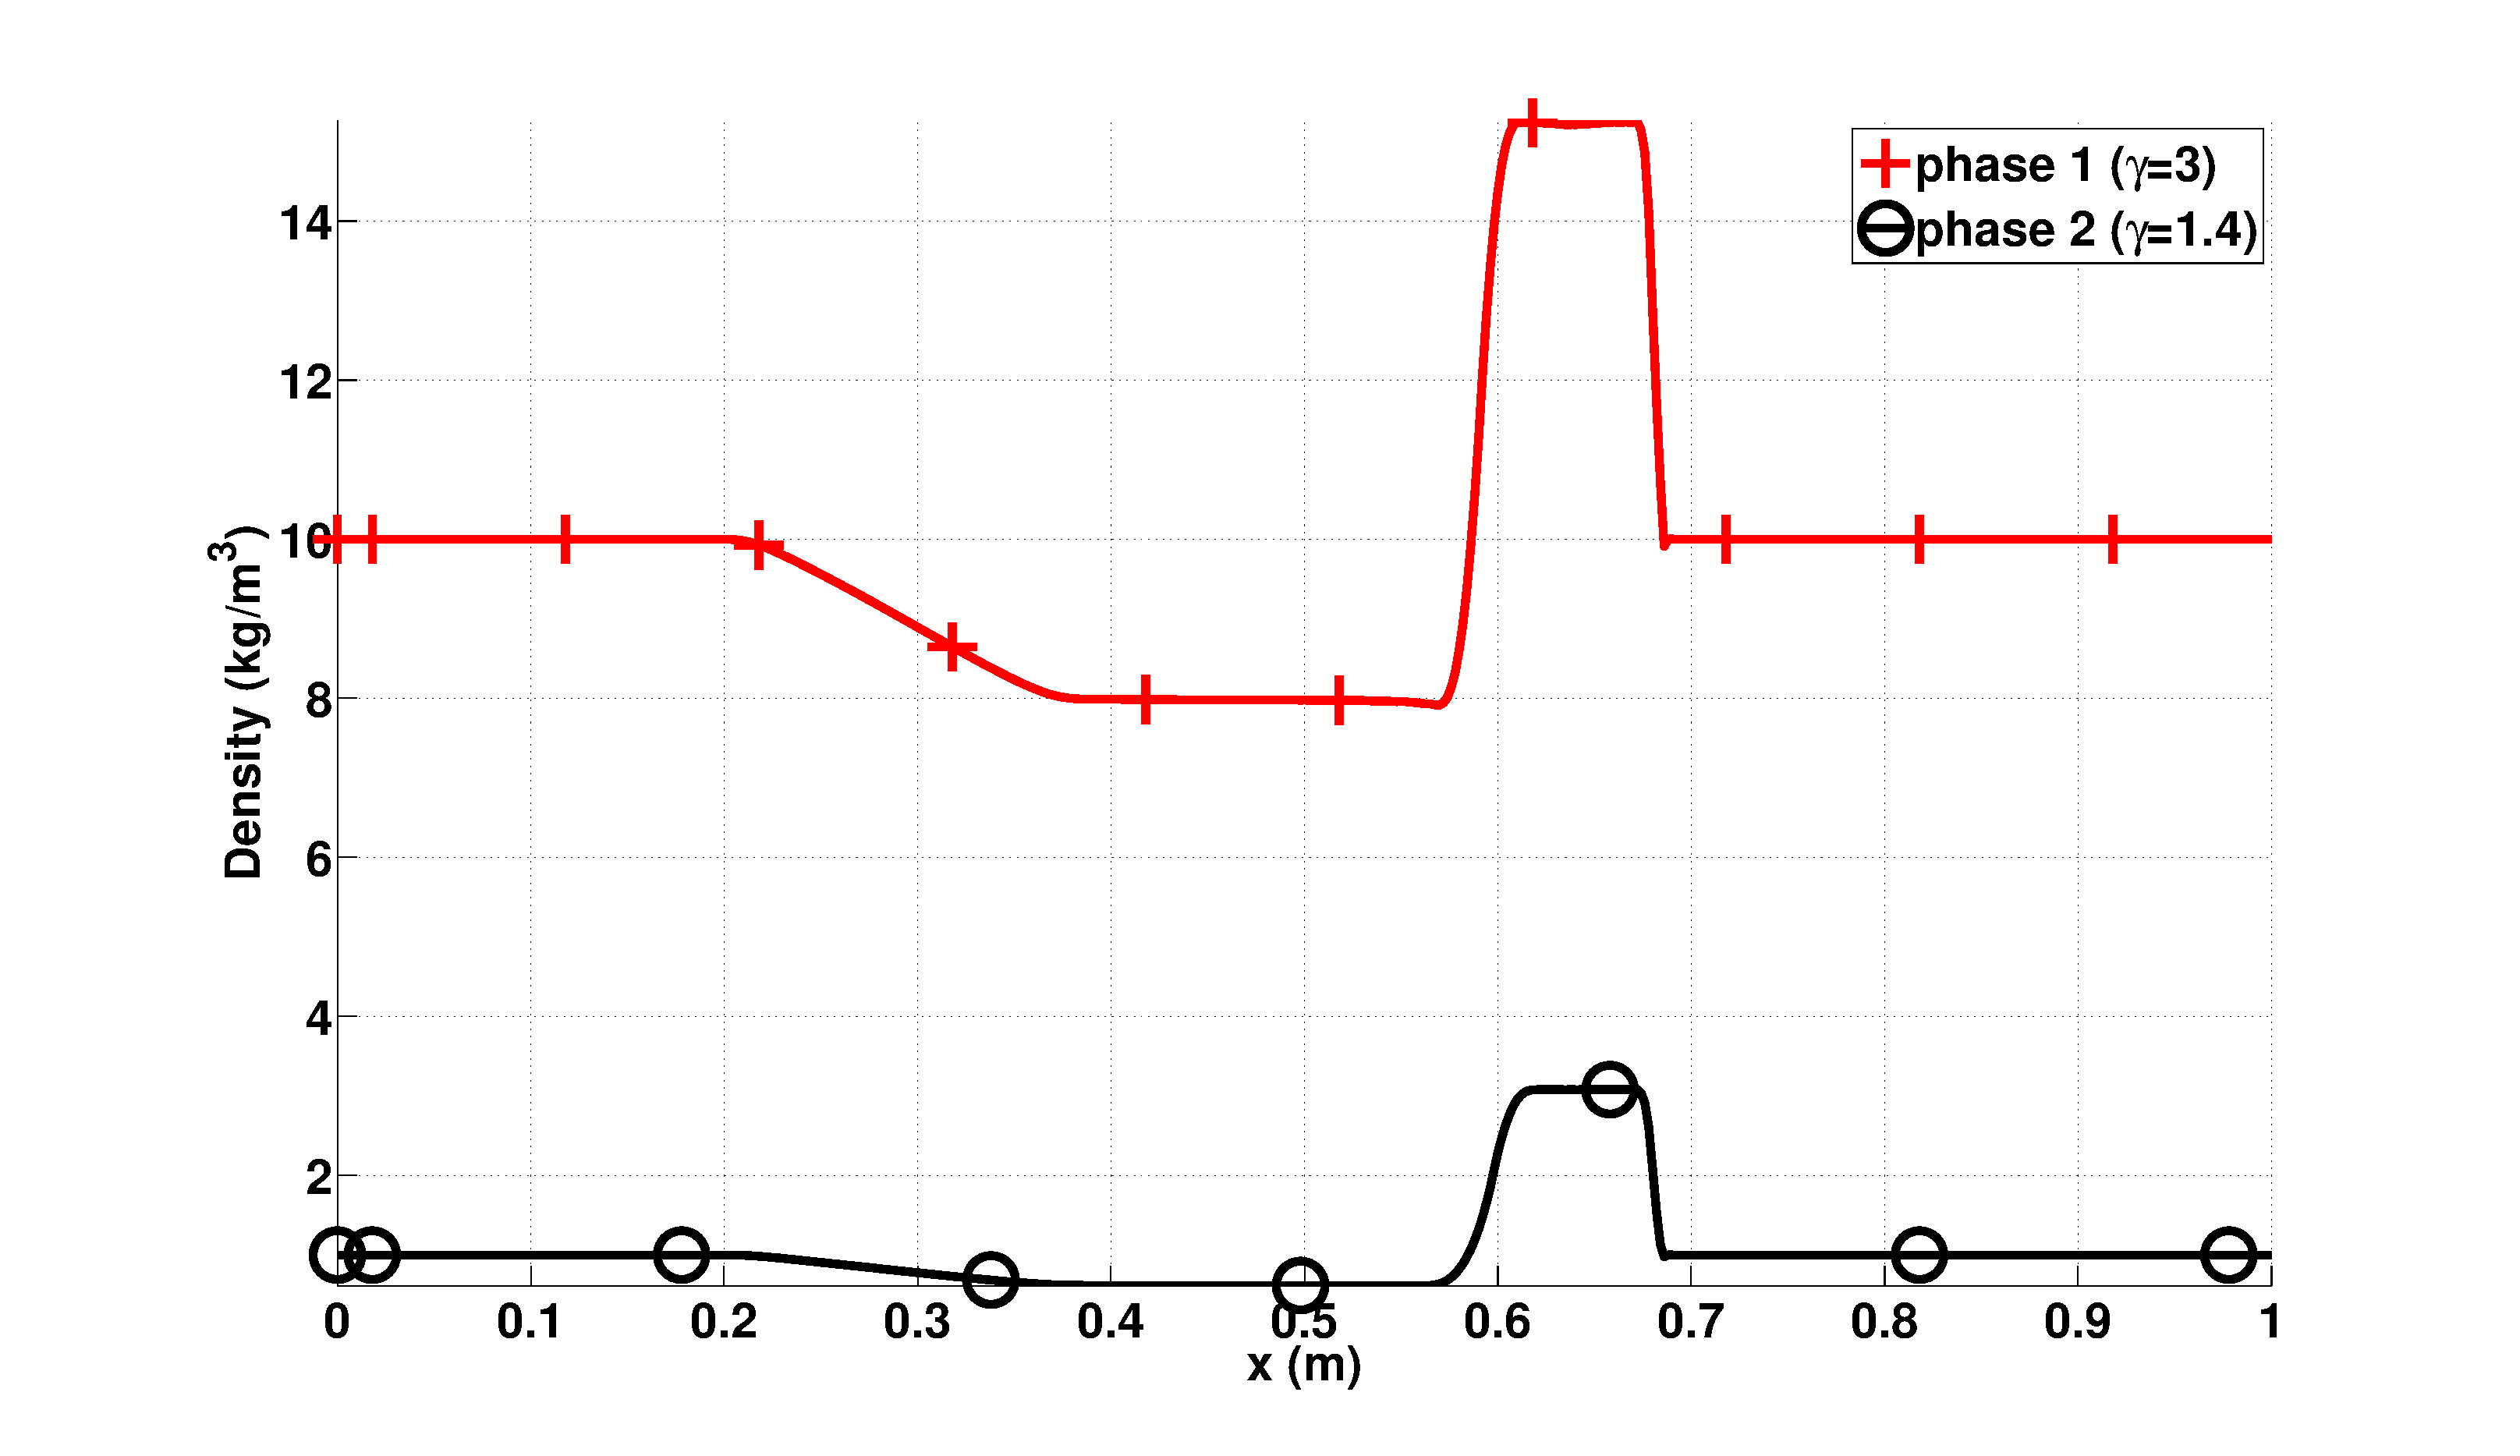
\includegraphics[width=0.31\textwidth]{figures_sem/relaxation_two_phases_density.eps}
}
\subfigure[Pressures]{
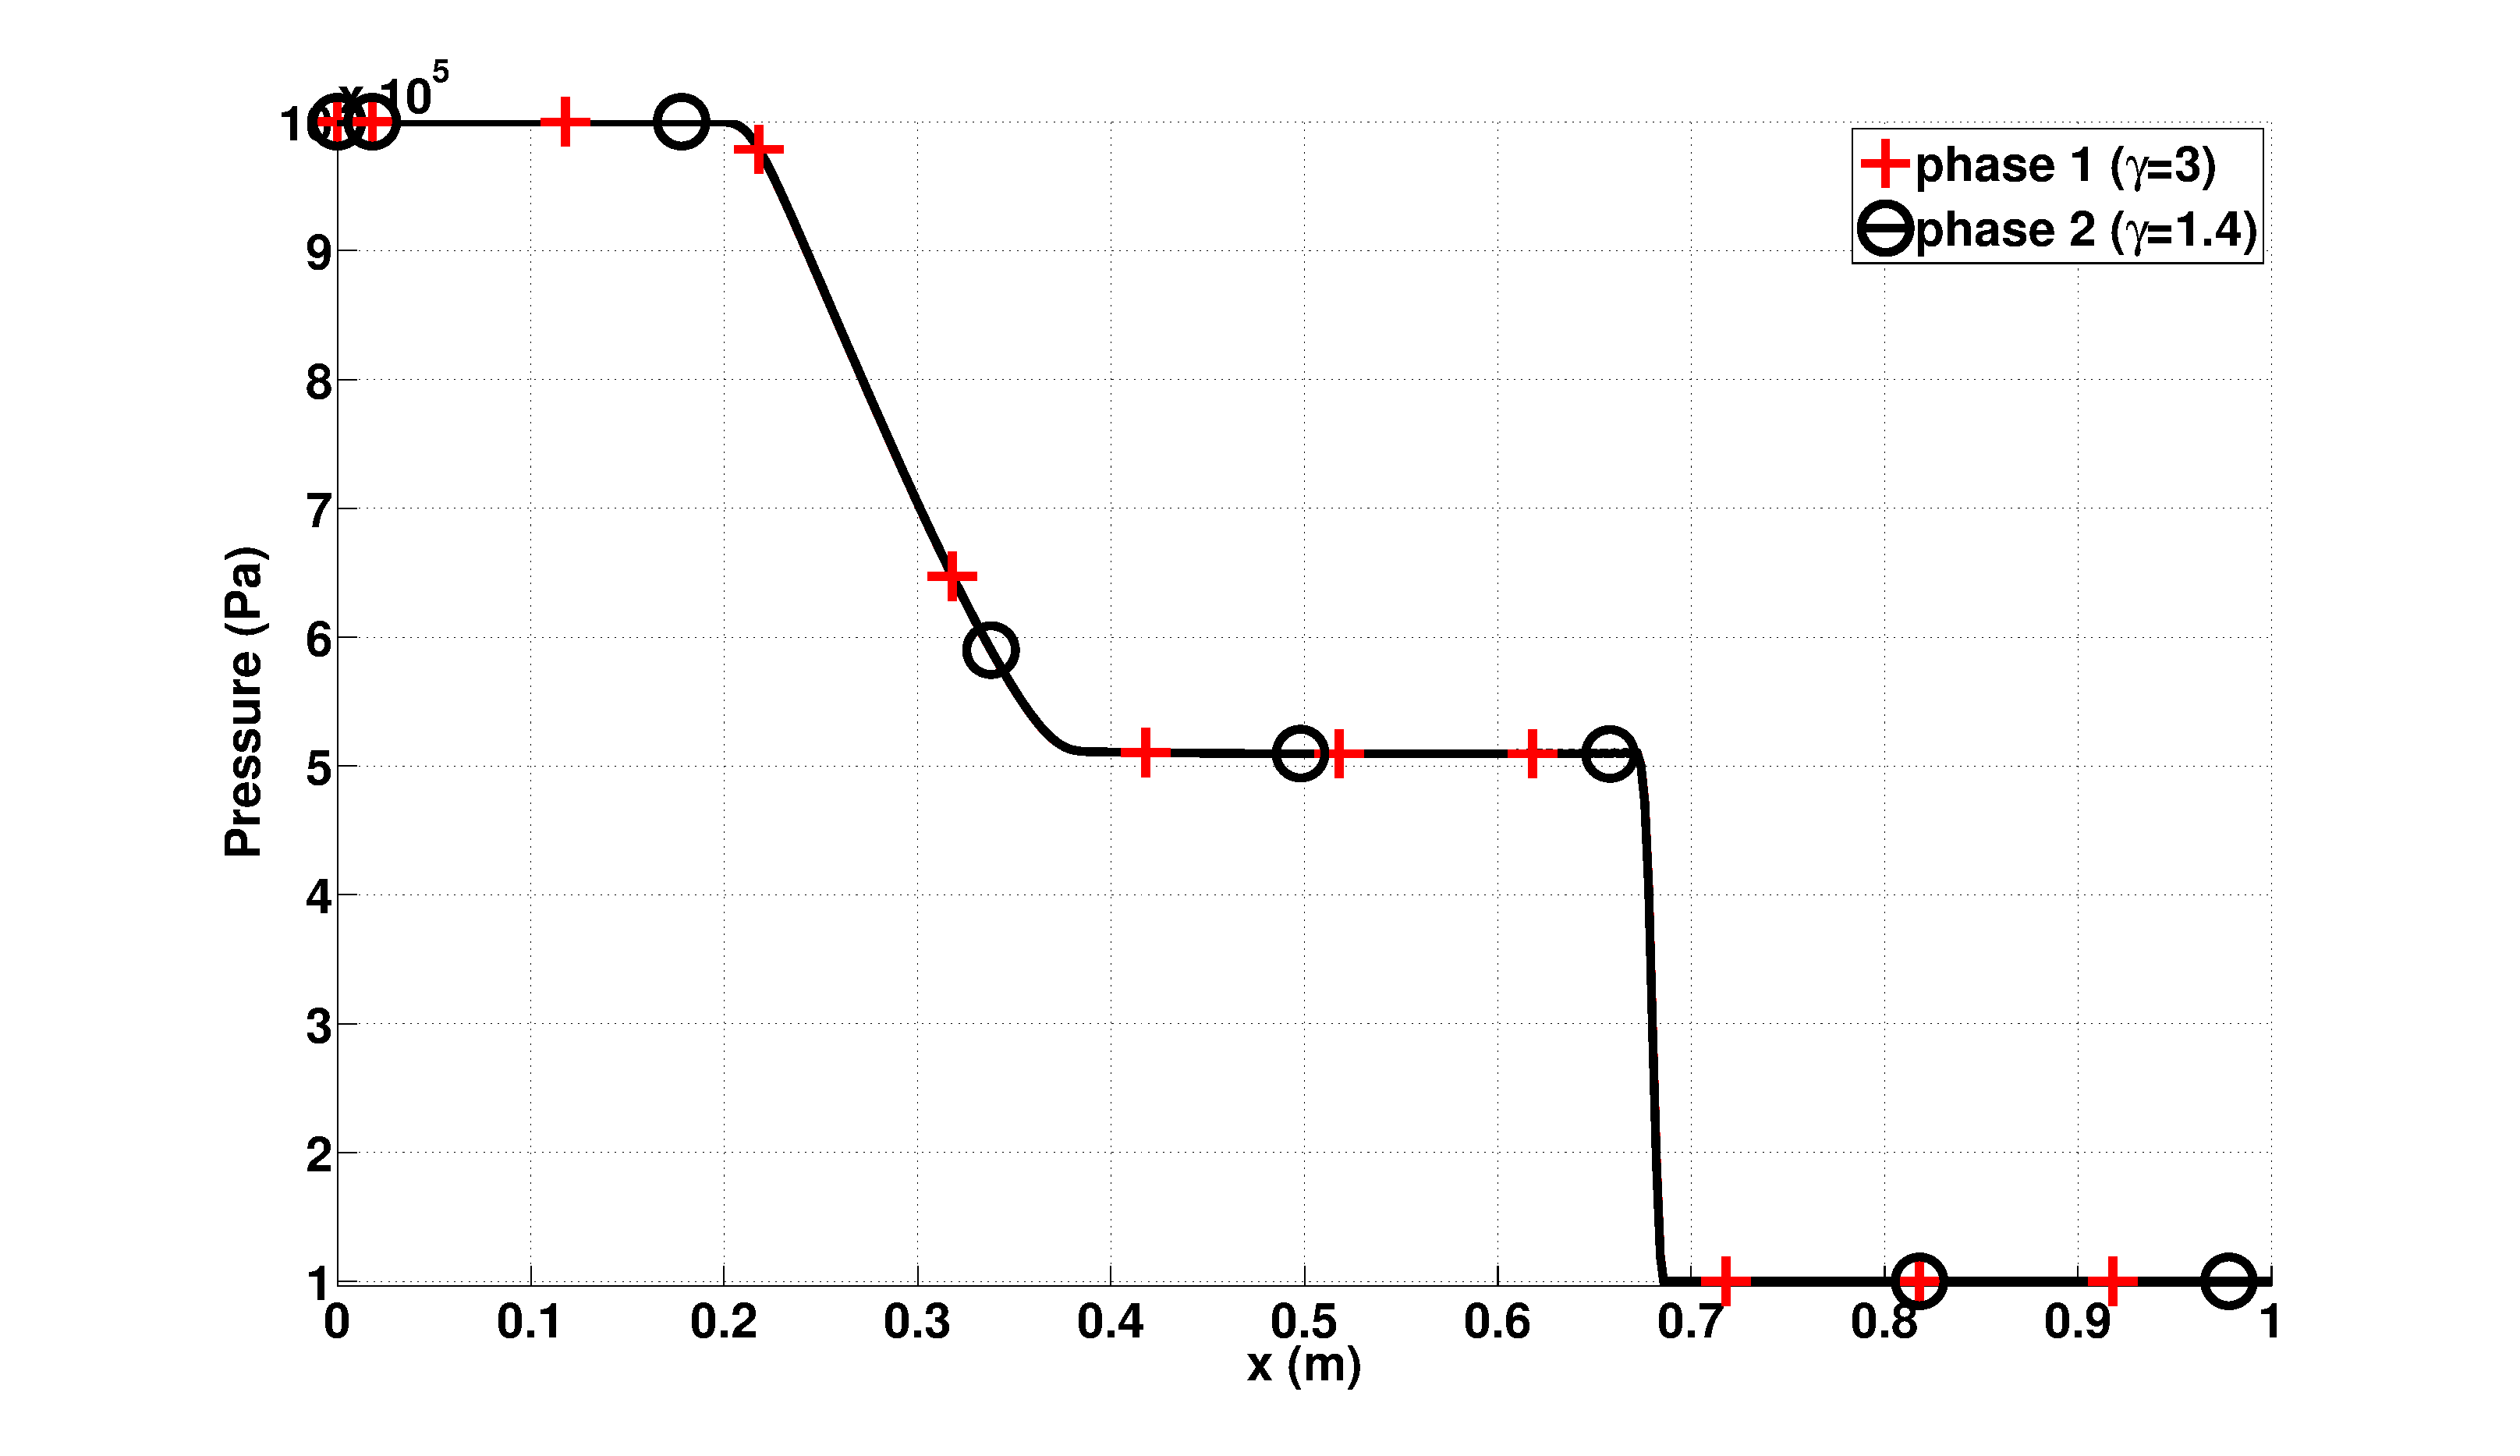
\includegraphics[width=0.31\textwidth]{figures_sem/relaxation_two_phases_pressure.eps}
}
\subfigure[Volume fractions]{
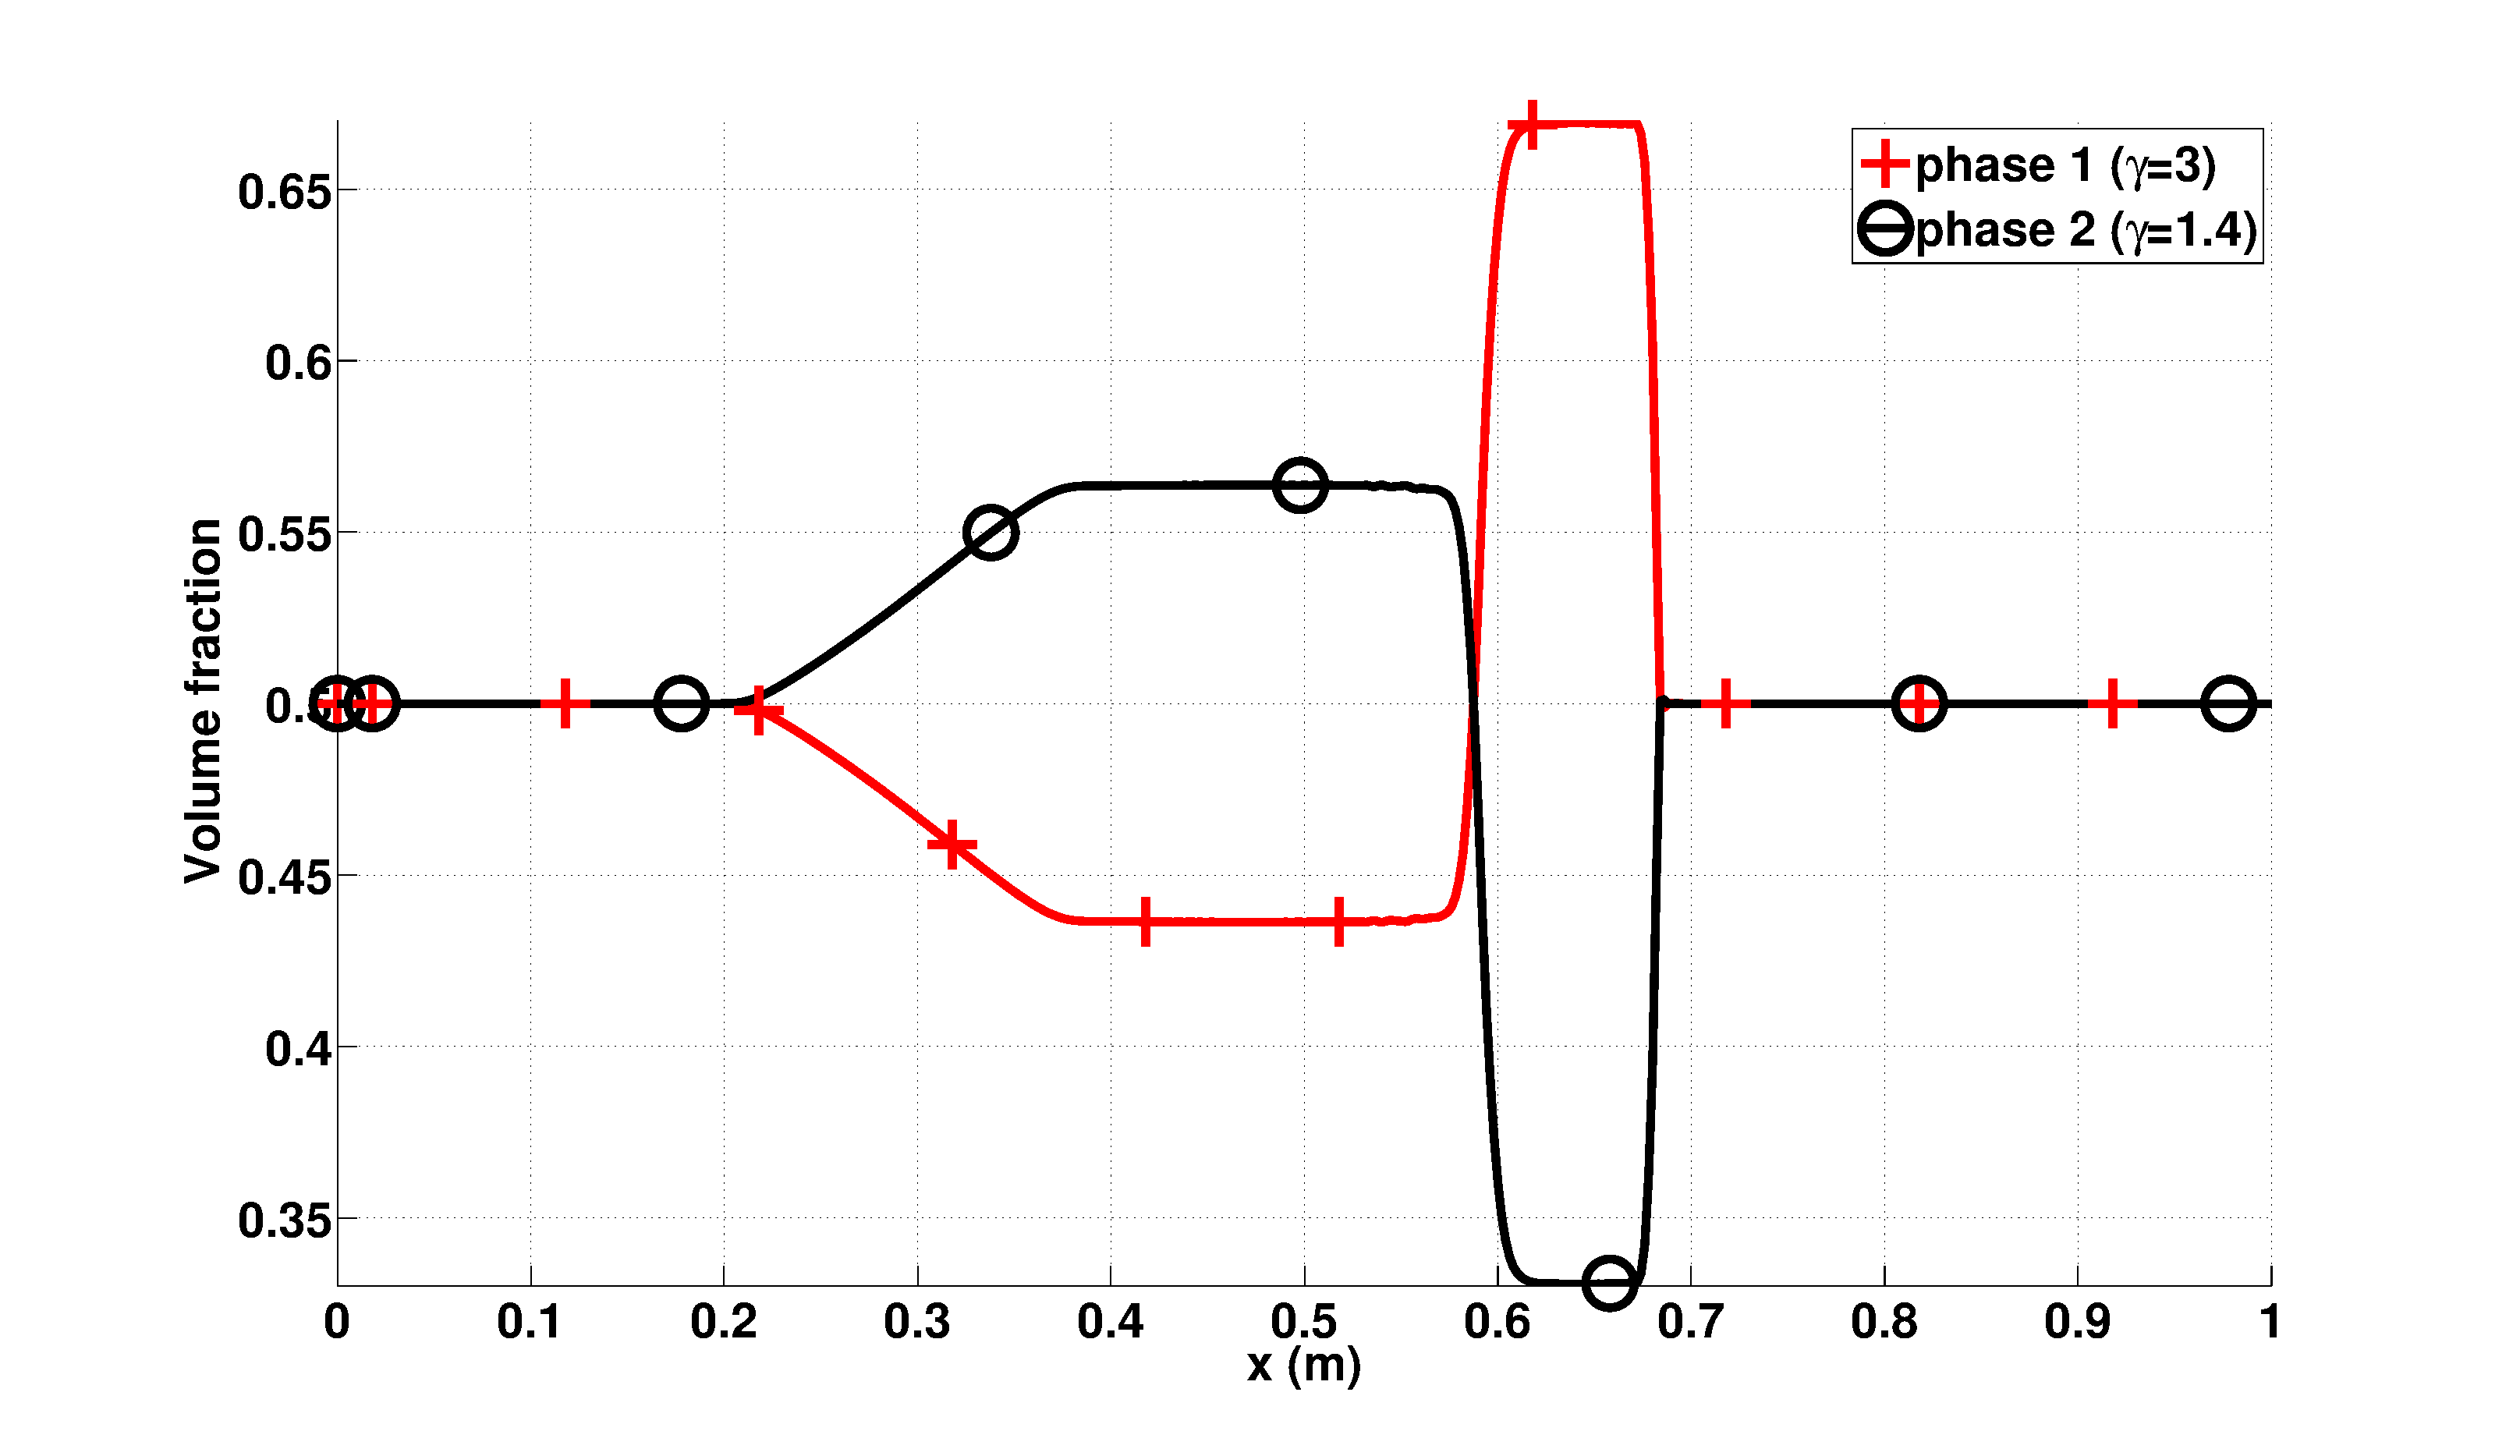
\includegraphics[width=0.31\textwidth]{figures_sem/relaxation_two_phases_volume_fraction.eps}
}
\\
\vspace{-3mm}
%
\subfigure[Viscosity $\kappa$, $\mu$ phase 1]{
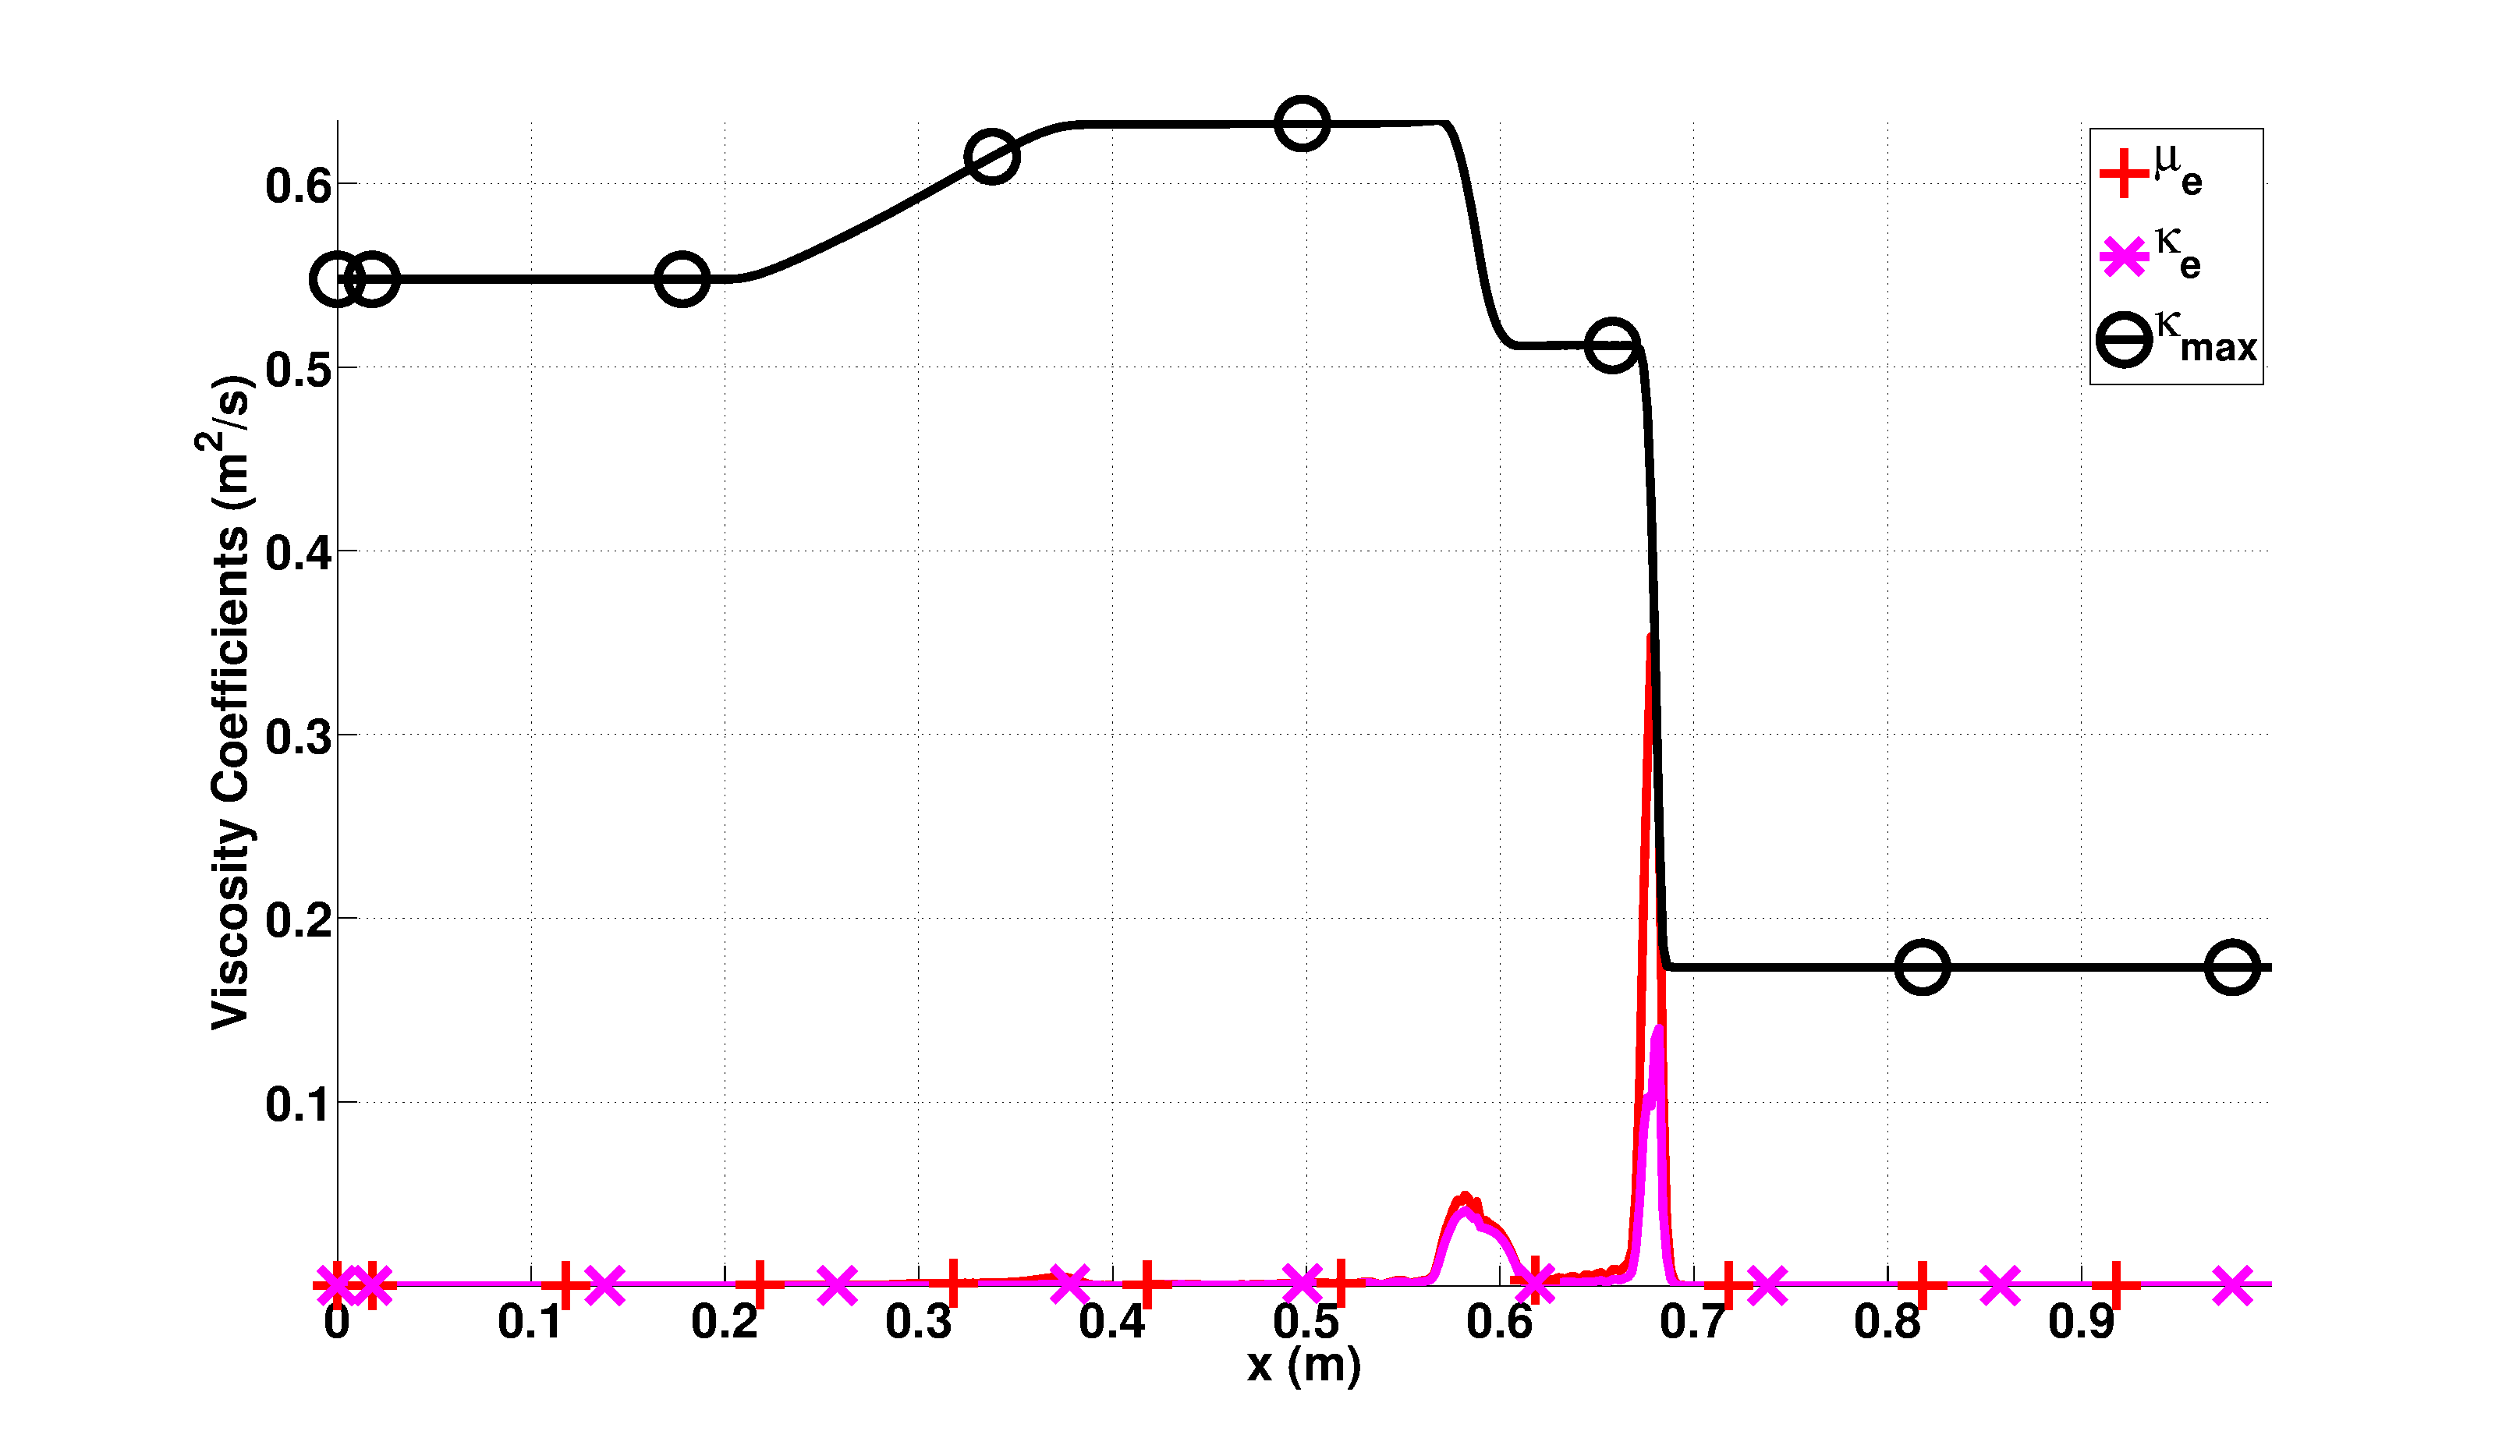
\includegraphics[width=0.31\textwidth]{figures_sem/relaxation_phase_1_viscosity_kappa_mu.eps}
}
\subfigure[Viscosity $\kappa$, $\mu$ phase 1]{
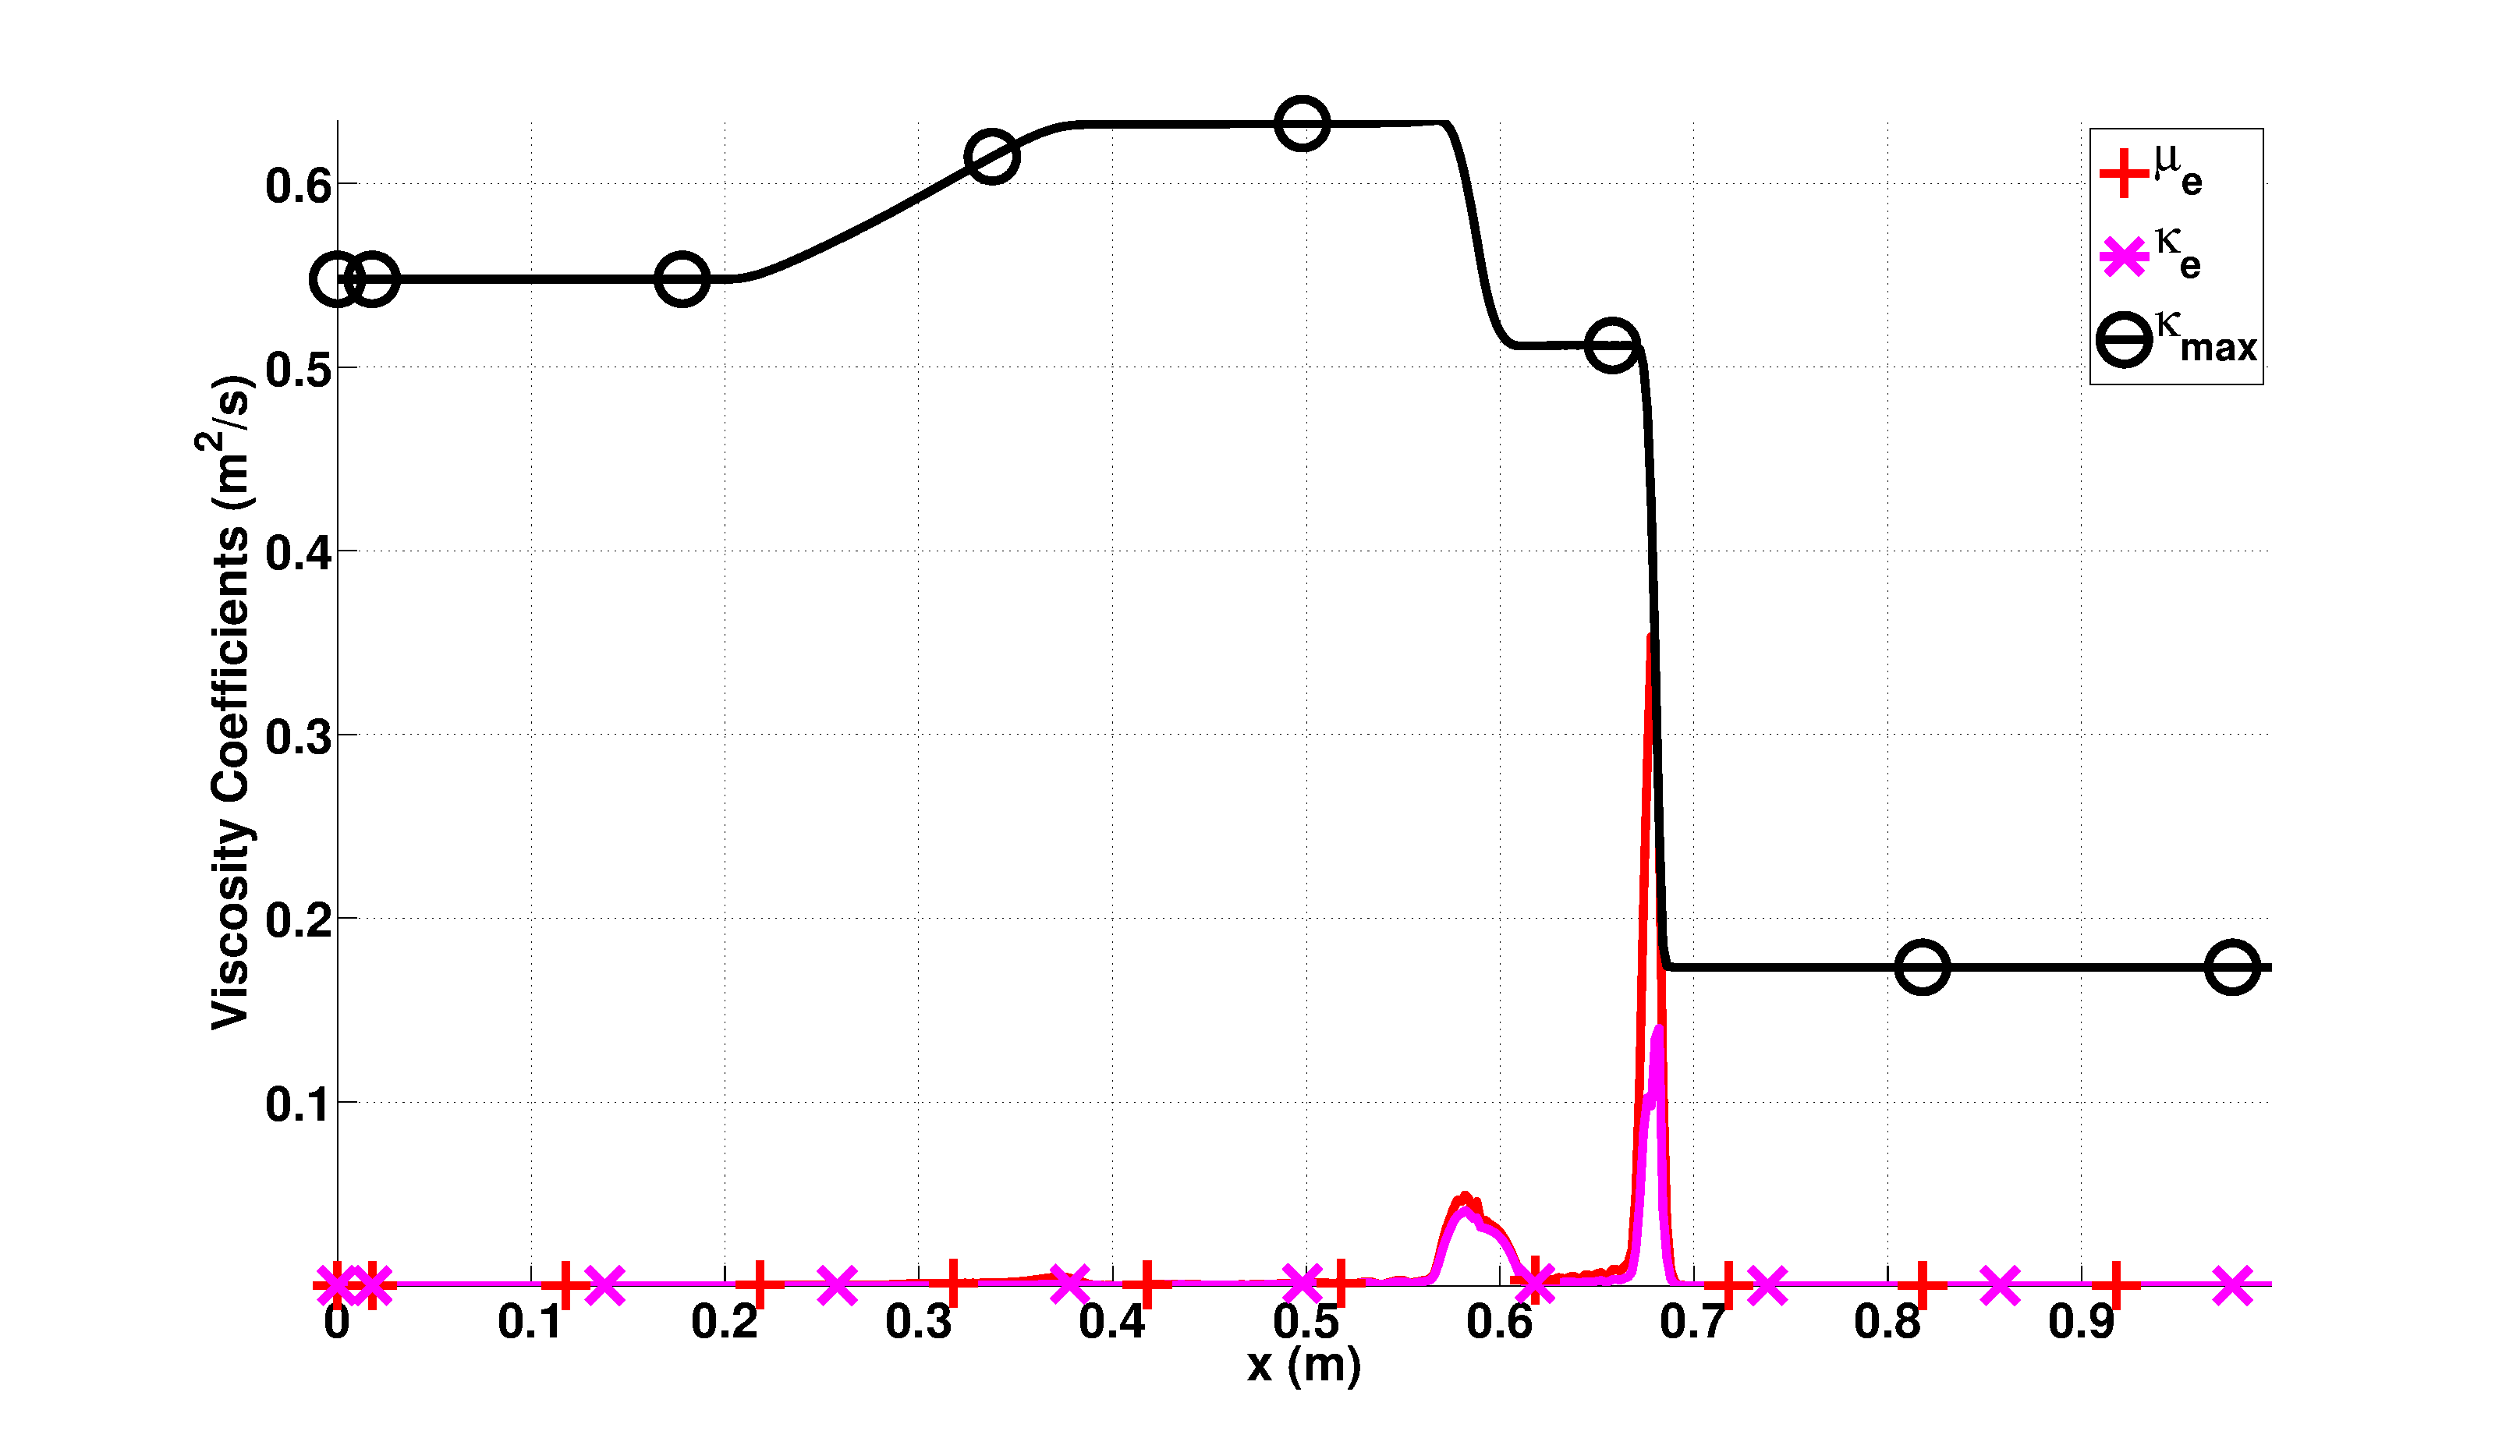
\includegraphics[width=0.31\textwidth]{figures_sem/relaxation_phase_1_viscosity_kappa_mu.eps}
}
\subfigure[Viscosity $\beta$ (volume fraction)]{
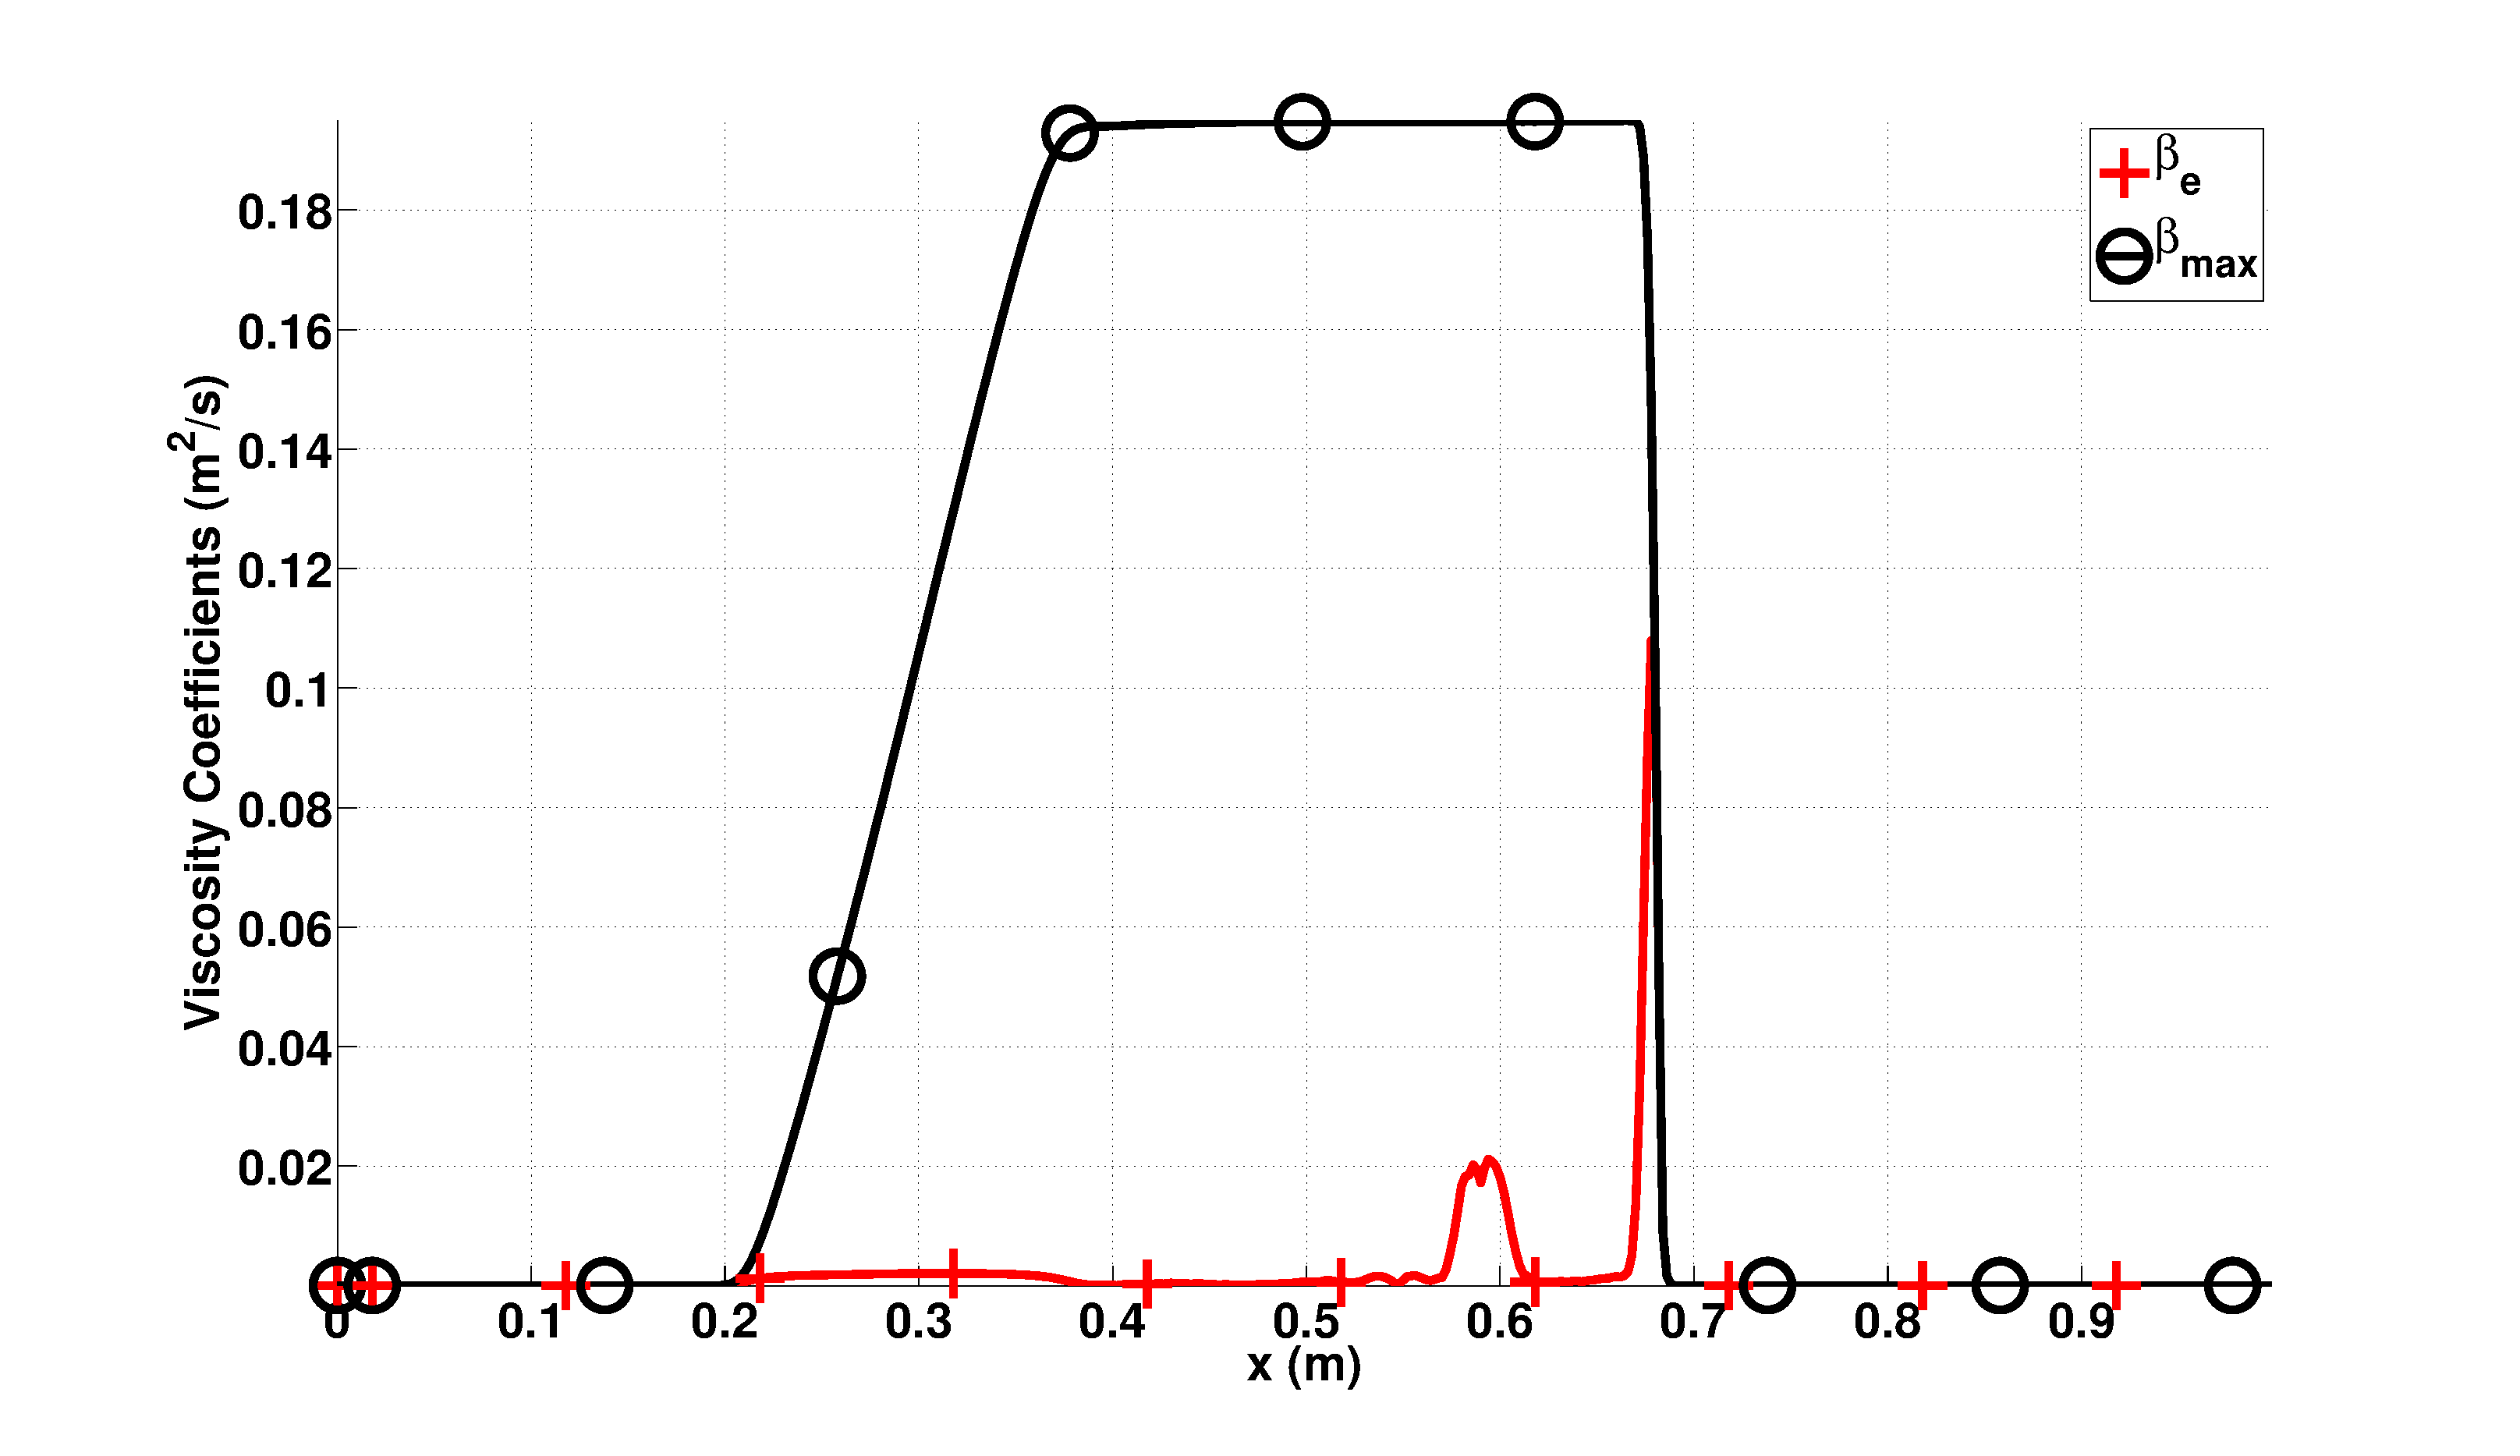
\includegraphics[width=0.31\textwidth]{figures_sem/relaxation_phase_1_beta.eps}
}
\end{figure}


\end{frame}
%%%%%%%%%%%%%%%%%%%%%%%%%%%%%%%%%%%%%%%%%%%%%%%%%%%%%%%%%%%%%%%%%%%%



%%%%%%%%%%%%%%%%%%%%%%%%%%%%%%%%%%%%%%%%%%%%%%%%%%%%%%%%%%%%%%%%%%%%
\begin{frame}[noframenumbering]{Thank you}
\label{lastslide}
\centering
Thanks to Jim Ferguson (LANL) for the semi-analytical solutions.\\
Thanks Jean-Luc Guermond and Bojan Popov (Texas A\&M) for fruitful discussions.

\begin{figure}
	\centering
	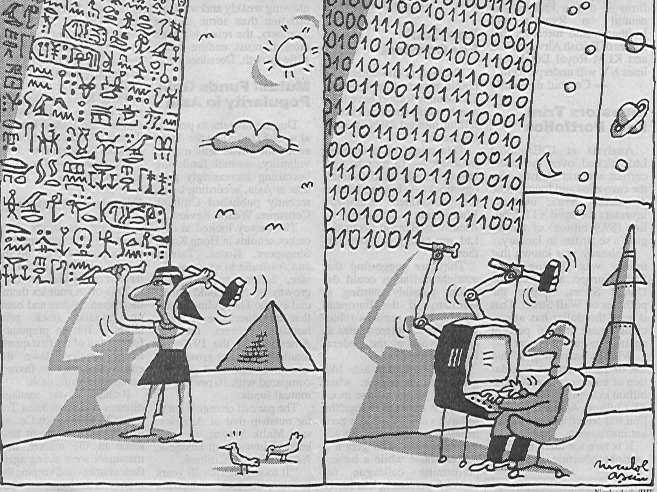
\includegraphics[scale=0.33]{./crunching.png}
\end{figure}

\end{frame}
%%%%%%%%%%%%%%%%%%%%%%%%%%%%%%%%%%%%%%%%%%%%%%%%%%%%%%%%%%%%%%%%%%%%


%%%%%%%%%%%%%%%%%%%%%%%%%%%%%%%%%%%%%%%%%%%%%%%%%%%%%%%%%%%%%%%%%%%%
\begin{frame}[noframenumbering]{Why an upper bound for viscosity?}

\begin{block}{}
Large entropy residual in shocks $\longrightarrow$ large entropy viscosity $\mu_e$ \\
\begin{center}
There is such a thing as too much of a good thing ...\\
{\it Il ne faut point \^{e}tre plus royaliste que le Roy}
\end{center}
\end{block}


\begin{block}{Upper bound for $\mu$}
First-order upwind scheme is monotone but over dissipative. We should not exceed the amount of stabilization that such a scheme provides.\\
\medskip
upwinding = \textcolor{blue}{centered approximation (Galerkin)} $-$ \textcolor{magenta}{numerical diffusion}\\
\underline{Example: linear advection} $\partial_t u + \beta \partial_x u =0$
\be
\beta \frac{u_i - u_{i-1}}{h} = \textcolor{blue}{\beta\frac{ u_{i+1}- u_{i-1}}{2h}} - \textcolor{red}{\frac{\beta h}{2}}
\textcolor{magenta}{\frac{ u_{i+1}-2u_i +u_{i-1}}{h^2}}
\ee
So, the dissipative term is $\frac{\beta h}{2}\partial_{xx} u$
and the first-order viscosity is $\frac{\beta h}{2}$
\end{block}

\begin{block}{First-order viscosity}
\hspace{0.5cm} $\bullet$ scalar conservation law: $\frac{h}{2}|f'(u)|$
\hspace{0.5cm} $\bullet$ system: $\frac{h}{2} \max \left( \text{eig}( \partial_u f) \right) $
\end{block}


\end{frame}
%%%%%%%%%%%%%%%%%%%%%%%%%%%%%%%%%%%%%%%%%%%%%%%%%%%%%%%%%%%%%%%%%%%%

%%%%%%%%%%%%%%%%%%%%%%%%%%%%%%%%%%%%%%%%%%%%%%%%%%%%%%%%%%%%%%%%%%%%
%%%%%%%%%%%%%%%%%%%%%%%%%%%%%%%%%%%%%%%%%%%%%%%%%%%%%%%%%%%%%%%%%%%%
\end{document}
